\documentclass[aspectratio=169,t,xcolor=table]{beamer}

\setlength{\itemsep}{0pt}
\setlength{\parskip}{0pt}
\setlength{\parsep}{0pt}

\usetheme{Finalyear}

% Theorems
\newtheorem{conj}{Conjecture}
\newtheorem{defi}{Definition}
\newtheorem{teo}{Theorem}
\newtheorem{lema}{Lemma}
\newtheorem{prop}{Proposition}
\newtheorem{cor}{Corollary}
\newtheorem{ex}{Example}
\newtheorem{exer}{Exercise}

\setbeamertemplate{theorems}[numbered]
\setbeamertemplate{caption}[numbered]

\setPrimaryColor{MyBlue}

\setLogos{lib/logo/iist-logo-horizontal.png}{lib/logo/iist-logo-square.png}

\graphicspath{%
  {../chapters/Figs/}%
  {images/}%
}

% Title Information
\begin{document}
\title[Post-Landfall MD Sustainability]{Post-Landfall Sustainability
of Monsoon Depressions over India}
\subtitle{The Role of the Brown Ocean Effect, Orographic
Modulation\\by the Eastern Ghats, and Antecedent Soil Moisture}

\author[Harshit P. D.]{
  \footnotesize
  \hfill
  \begin{columns}
    \column{0.42\textwidth}
    \centering
    \textbf{Presented by:} \\
    \textbf{Harshit Prashant Dhanwalkar} \\
    SC21B164
    \column{0.42\textwidth}
    \centering
    \textbf{Supervisor:} \\
    Dr. A. Chandrasekar \\
    \small Outstanding Professor,  \\
    Dept. Earth System Sciences
  \end{columns}
  \hfill
}

\date{May 2026}
\frame[noframenumbering]{\titlepage}

% OUTLINE
\setLayout{vertical}
\begin{frame}{Presentation Outline}
  \footnotesize
  \begin{columns}
    \column{0.48\textwidth}
    \textbf{\small Part I Background \& Methods}
    \begin{itemize}
      \item The post-landfall problem
      \item Brown Ocean Effect mechanism
      \item Research objectives \& dataset
      \item Azimuthal Hovmöller framework
    \end{itemize}

    \vspace{0.4cm}

    \textbf{\small Part II Climatological Results}
    \begin{itemize}
      \item 2001-2025 track database
      \item Interannual trends \& duration distribution
      \item Spatial distribution of tracks
    \end{itemize}

    \column{0.48\textwidth}
    \textbf{\small Part III Process-level Results}
    \begin{itemize}
      \item Precipitation dynamics (Hovmöller)
      \item Soil moisture \& LHF signals
      \item SHF \& dew-point diagnostics
      \item Eastern Ghats - terrain vs. thermodynamics
      \item Surface energy time series
      \item Precipitation-soil moisture feedback
      \item Translational speed \& BOE survivors
    \end{itemize}

    \vspace{0.3cm}

    \textbf{\small Part IV Conclusions}
    \begin{itemize}
      \item BOE as a diagnostic mechanism
      \item Principal conclusions
      \item Future work \& applications
    \end{itemize}
  \end{columns}
\end{frame}

% SECTION I - BACKGROUND
\section{Background}
\setLayout{mainpoint}
\begin{frame}{}
  \frametitle{BACKGROUND}
\end{frame}

%---------------------------------------------------------Slide: The Problem
\setLayout{plain}
\begin{frame}{The Post-Landfall Problem: Why Do Some MDs Persist?}
  \begin{columns}
    \column{0.48\textwidth}
    \textbf{\small Monsoon Depressions (MDs):}
    \footnotesize
    \begin{itemize}
      \item Form over the Bay of Bengal (BoB) during JJAS; track NW at 2-10 m\,s$^{-1}$.
      \item Broad precipitation shield (500-800 km radius); contribute \textbf{50-60\%} of central India's seasonal rainfall.
      \item Classical theory: \textbf{decay within 24-48 h} after landfall - oceanic energy source removed, friction increases.
    \end{itemize}

    \vspace{0.2cm}

    \begin{alertblock}{\small The Anomaly}
      \footnotesize
      A significant fraction of observed MDs maintains organized 850
      hPa vorticity and deep convection for \textbf{3-5 days} and
      \textbf{800-1200 km inland}. The 2021 Odisha system and 2017
      Bihar floods are recent examples - each caused multi-day
      flooding affecting millions.
    \end{alertblock}

    \column{0.52\textwidth}
    \vspace{-0.9cm}
    \begin{figure}
      \centering
      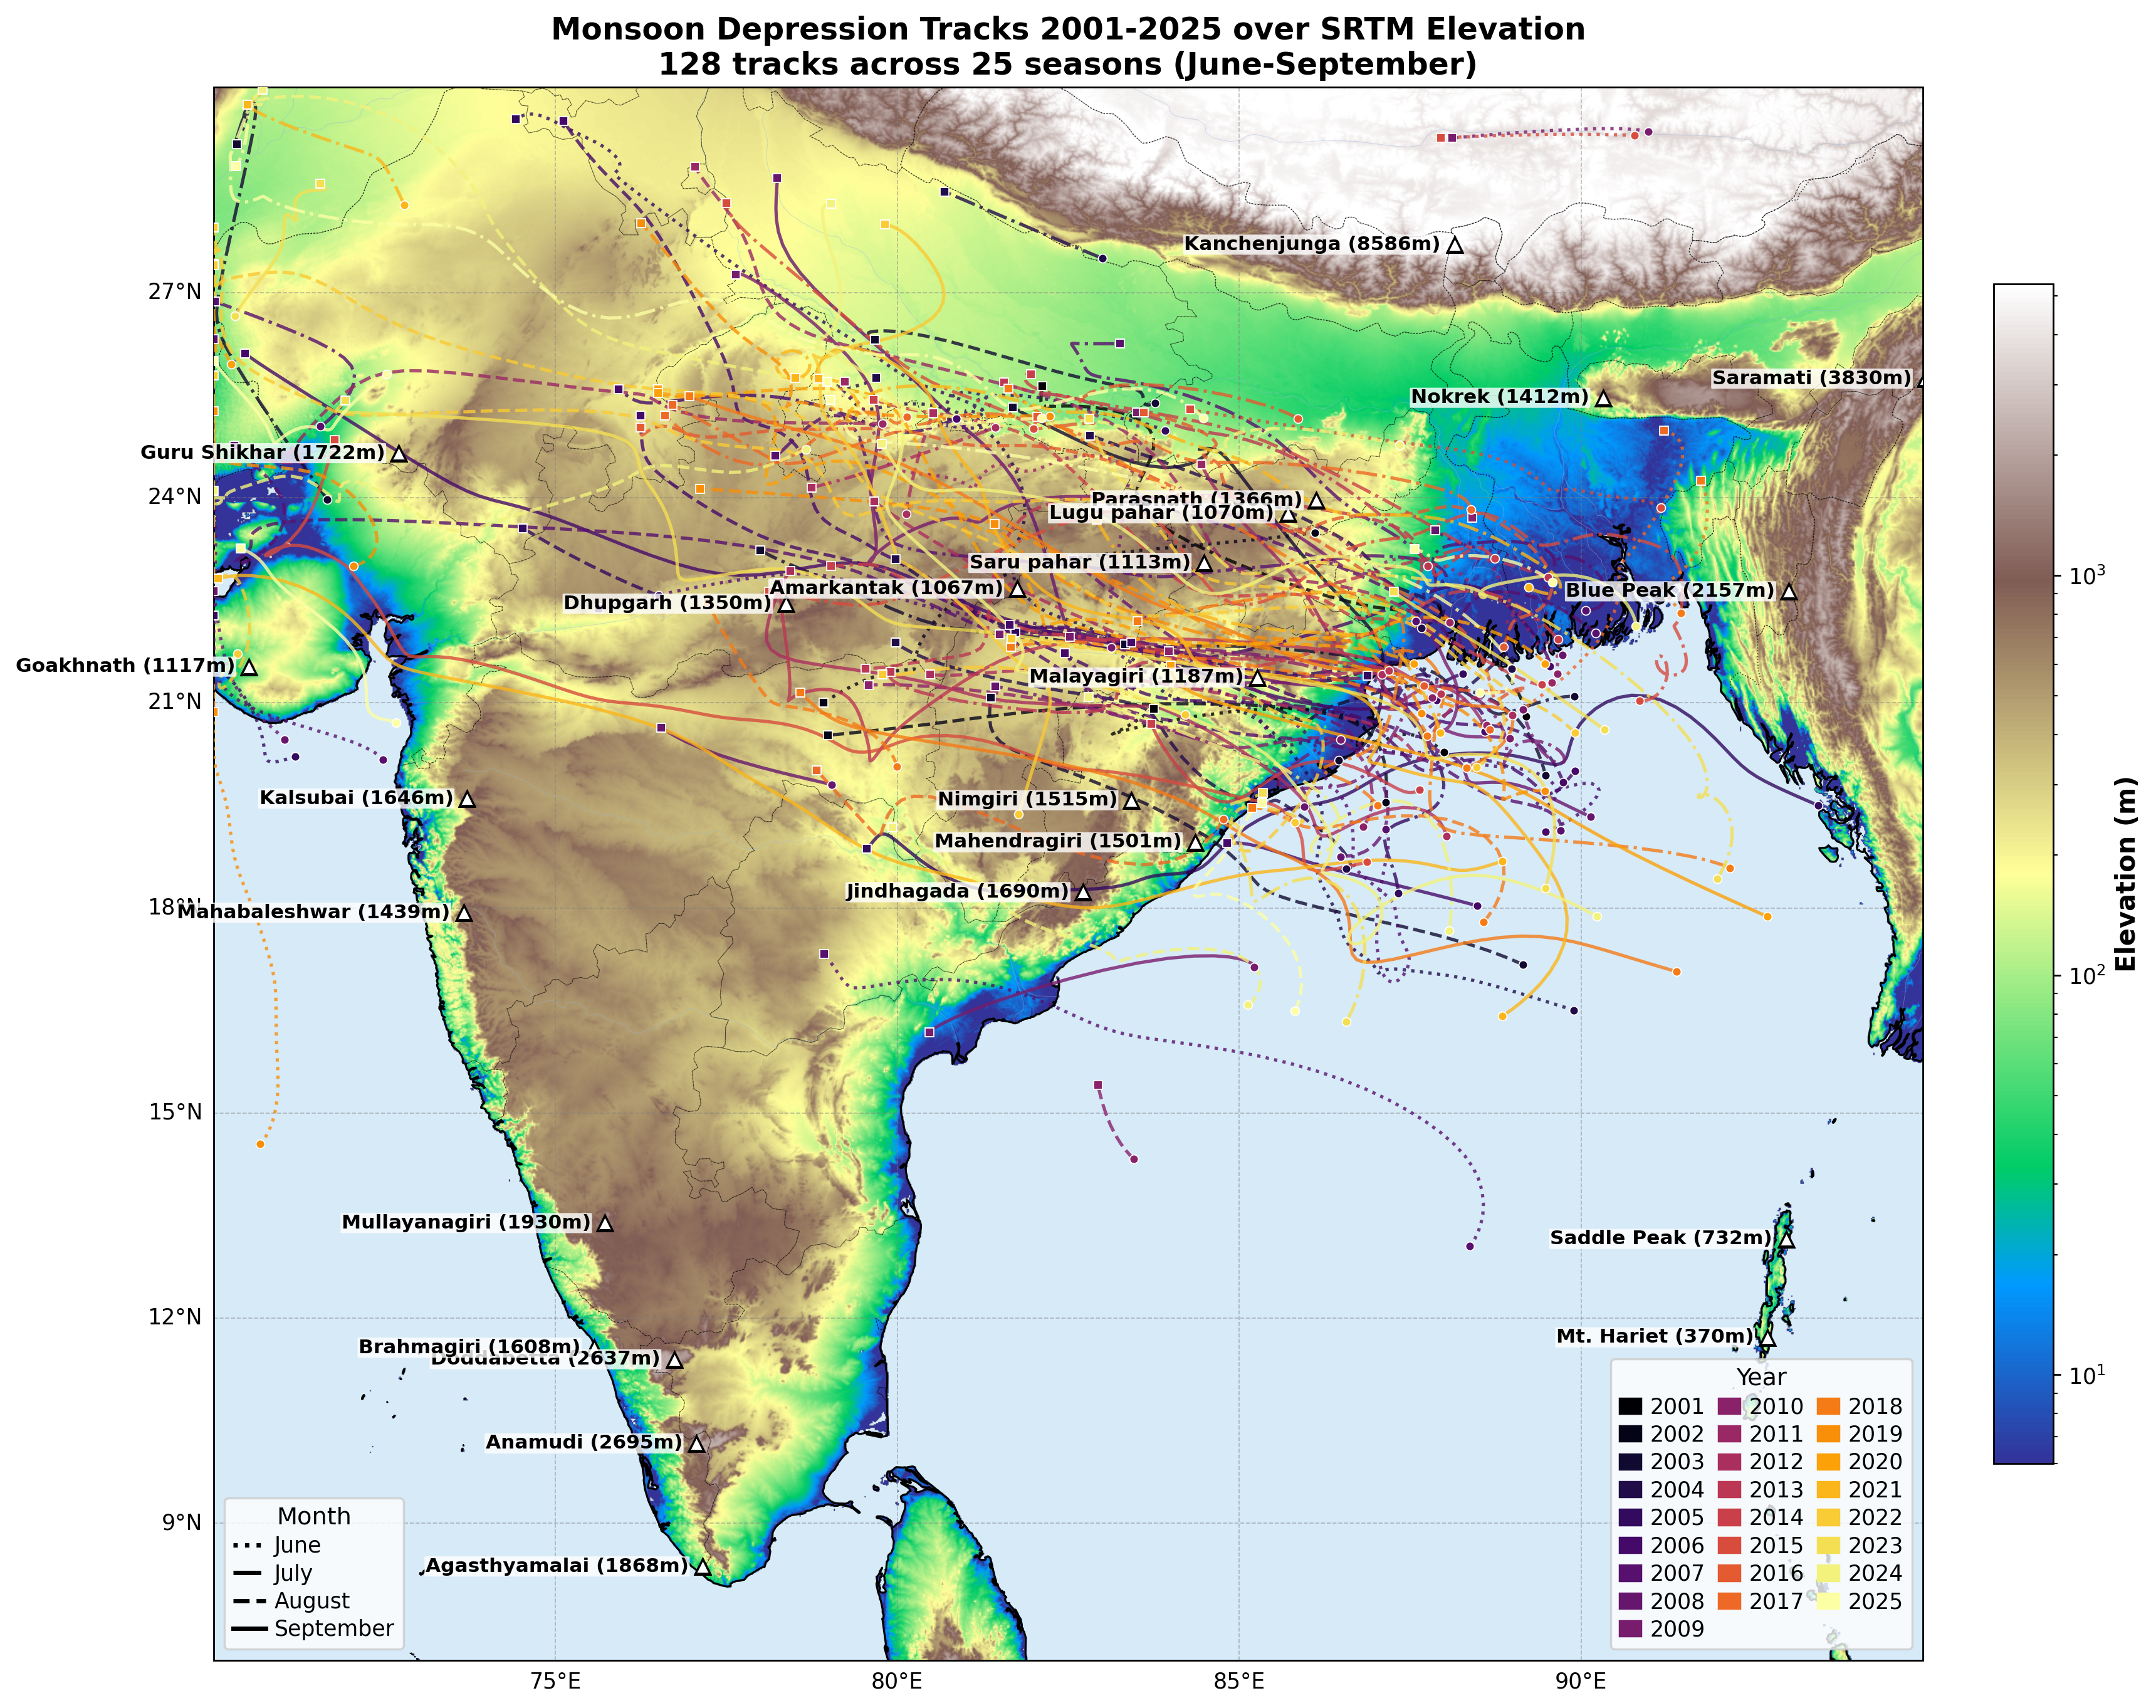
\includegraphics[width=\textwidth]{all_years_tracks_elevation_1}
      \caption{\scriptsize Schematic of a Monsoon Depressions and thier northwestward track over India, with SRTM elevation map and some of high mountain peaks.}
    \end{figure}
  \end{columns}
\end{frame}

%---------------------------------------------------------Slide: BOE Mechanism
\setLayout{plain}
\begin{frame}{The Brown Ocean Effect (BOE): Mechanism}
  \begin{columns}
    \column{0.46\textwidth}
    \textbf{\small What is the BOE?}
    \footnotesize
    \begin{itemize}
      \item First named by \textit{Andersen \& Shepherd (2013)}: a
        saturated land surface mimics the energetic behaviour of a
        warm tropical ocean
      \item Pre-moistened soil evaporates at the \textbf{potential
        evaporation rate} - water supply is not limiting
      \item Result: high LHF, low Bowen ratio ($\beta = Q_H/Q_E
        \approx 0.1$), near-saturated boundary layer
    \end{itemize}

    \column{0.53\textwidth}
    \vspace{-0.6cm}
    \begin{figure}
      \centering
      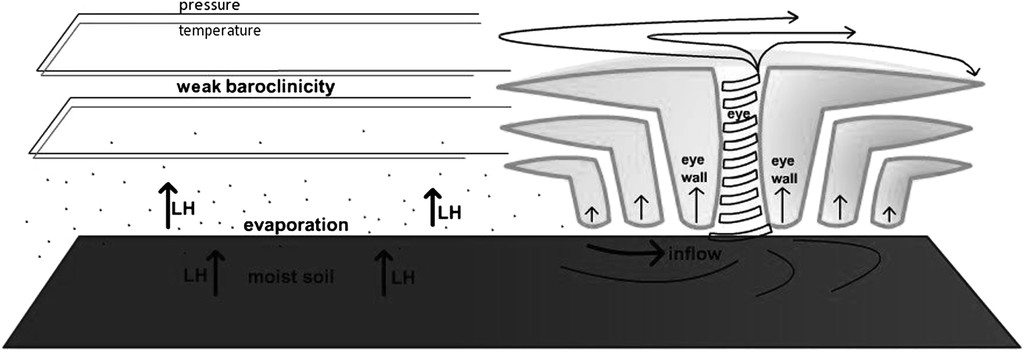
\includegraphics[width=0.98\textwidth]{BOE_schematic}
      \caption{\footnotesize The Brown Ocean Effect: saturated soil
        sustains LHF $\geq 70$ W\,m$^{-2}$, maintaining the
        precipitation-soil moisture positive feedback. \textit{Source:
      Andersen \& Shepherd (2013).}}
    \end{figure}
  \end{columns}

  \vspace{0.5cm}

  \textbf{\small The Self-Reinforcing Loop:}
  \footnotesize
  \[
    \text{MD rainfall} \rightarrow \text{Soil saturation} \rightarrow
    \text{High LHF} \rightarrow \text{Sustained convection}
    \rightarrow \text{More rainfall}
  \]
\end{frame}

%---------------------------------------------------------Slide:
% Research Objectives + Data
\setLayout{vertical}
\begin{frame}{Research Objectives \& Dataset}
  \begin{columns}
    \column{0.51\textwidth}
    \textbf{\small Research Objectives:}
    \footnotesize
    \begin{enumerate}
      \item \textbf{Detect \& characterise} MD events from ERA5 over
        2001-2025 (cross-validated against annual IMD monsoon
        reports); classify as short-lived ($<96$ h) or long-lived ($\geq 96$ h)
      \item \textbf{Reconstruct azimuthal \& radial evolution} of
        surface LHF, SHF, soil moisture (SWVL1), precipitation, and
        2-m dew-point via Azimuthal Hovmöller analysis
      \item \textbf{Quantify terrain influence} - Eastern Ghats
        effect on translational speed, precipitation asymmetry, and
        inland penetration; identified how terrain-BOE interaction
        modulates longevity
    \end{enumerate}

\column{0.48\textwidth}
    \textbf{\small Dataset:}
    \footnotesize
    \begin{itemize}
      \item \textbf{ERA5 Reanalysis} (ECMWF): $0.25^\circ \times 0.25^\circ$, hourly, 2001-2025
      \item \textbf{Variables:} SWVL1, LHF (slhtf), SHF (ishf), Total Precip (tp), D2M, MSLP, 850 hPa vorticity
      \item \textbf{SRTM Elevation Data:} terrain analysis of Eastern Ghats interactions
      \item \textbf{Domain:} 5-35°N, 65-100°E
      \item \textbf{IMD Monsoon Seasonal Reports:} cross-validation of detected tracks
      \item \textbf{Period:} June-September, 2001-2025
    \end{itemize}

    \vspace{0.15cm}
    \tiny\textcolor{gray}{\textbf{Data Acknowledgments:} Track cross-validation utilizes official Monsoon Reports provided by the \textbf{India Meteorological Department (IMD)}. Topographic elevation metrics are derived from NASA's \textbf{Shuttle Radar Topography Mission (SRTM)} 90m dataset.}
  \end{columns}
\end{frame}

%---------------------------------------------------------Slide:
% Methodology - Azimuthal Hovmöller
\setLayout{plain}
\begin{frame}{Azimuthal Hovmöller Framework}
  \vspace{-0.3cm}
  \begin{columns}
    \column{0.57\textwidth}
    \textbf{\small Construction:}
    \footnotesize
    \begin{enumerate}
      \item MD center tracked hourly (850 hPa vorticity maximum)
      \item Polar grid: \textbf{25 km radial bins to 400 km}, divided
        into \textbf{16 azimuthal sectors} of 22.5° each
      \item ERA5 grid points averaged within each sector-annulus
        cell; then azimuthally averaged $\Rightarrow$ radial profile $H(r,t)$
      \item Time axis aligned at \textbf{landfall ($t = 0$)}; ocean
        phase ($t<0$), land phase ($t>0$)
    \end{enumerate}

    \vspace{0.1cm}

    \textbf{\small Variables in the framework:}
    \footnotesize
    \begin{itemize}
      \item Total precipitation (TP), Surface LHF, Surface SHF
      \item Near-surface soil moisture (SWVL1, 0-7 cm)
      \item 2-m Dew-point temperature (D2M)
    \end{itemize}

    \column{0.43\textwidth}
    \vspace{-0.6cm}
    \begin{figure}
      \centering
      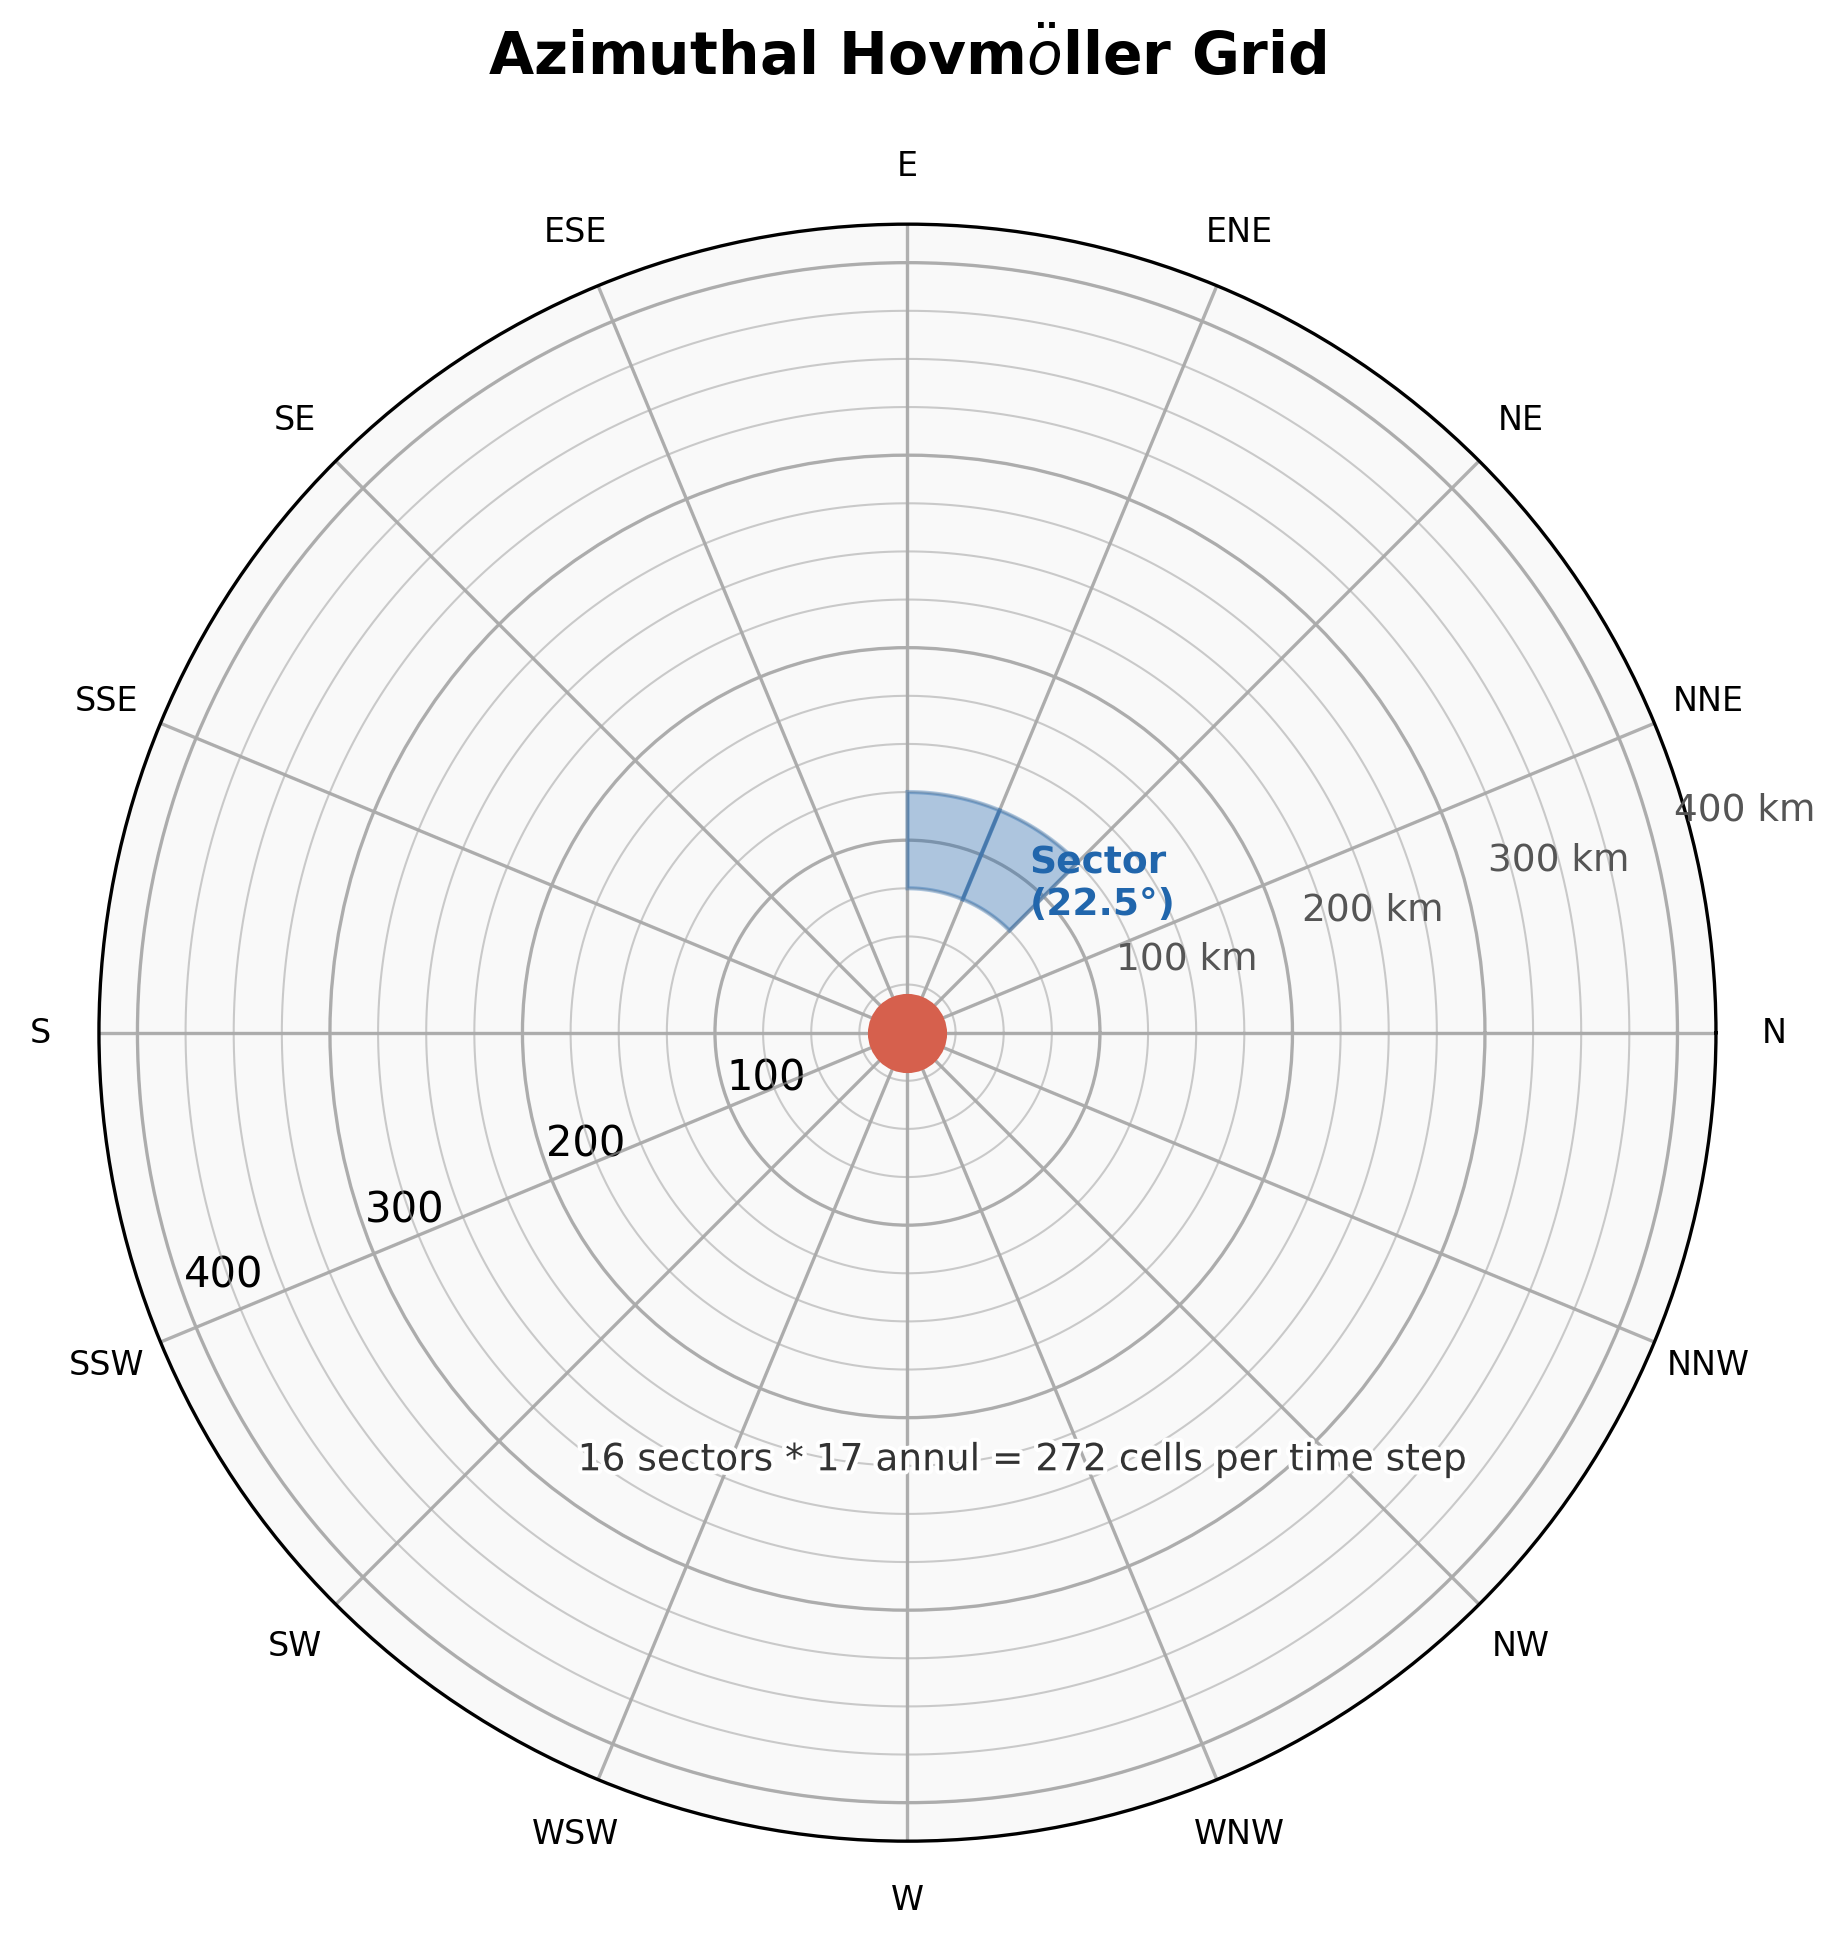
\includegraphics[width=0.90\textwidth]{hovmoller_geometry.png}
      \caption{\footnotesize Polar grid for Azimuthal Hovmöller: 25
      km radial bins to 400 km, 16 sectors of 22.5° each.}
    \end{figure}
  \end{columns}
\end{frame}

% SECTION II - CLIMATOLOGICAL RESULTS
\section{Climatological Results}
\setLayout{mainpoint}
\begin{frame}{}
  \frametitle{RESULTS: CLIMATOLOGY 2001-2025}
\end{frame}

% ---------------------------------------------------------Slide: Track Database
\setLayout{vertical}
\begin{frame}{Track Database: 2001-2025}
  \begin{columns}
    \column{0.43\textwidth}
    \textbf{\small Summary Statistics:}
    \vspace{-0.3cm}
    \footnotesize
    \begin{center}
      \begin{tabular}{lccc}
        \toprule
        \rowcolor{MyBlue!20}
        \textbf{Statistic} & \textbf{All} & \textbf{Short} & \textbf{Long} \\
        \midrule
        No. of MDs& 128 & 90 & 38 \\
        \rowcolor{MyBlue!10}
        Mean duration (h) & 79.4 & 54.6 & 138.3 \\
        Std. deviation (h) & 44.2 & 19.1 & 27.9 \\
        \rowcolor{MyBlue!10}
        \% of total & 100\% & 70.3\% & \textbf{29.7\%} \\
        \bottomrule
      \end{tabular}
    \end{center}

    \vspace{0.3cm}
    \begin{alertblock}{\small BOE Classification}
      \footnotesize
      \textbf{All 38 long-lived systems} meet the BOE criterion
      (inland LHF $\geq 70$ W\,m$^{-2}$ for $\geq 18$ h).
    \end{alertblock}

    \column{0.56\textwidth}
    \vspace{-0.7cm}
    \begin{figure}
      \centering
      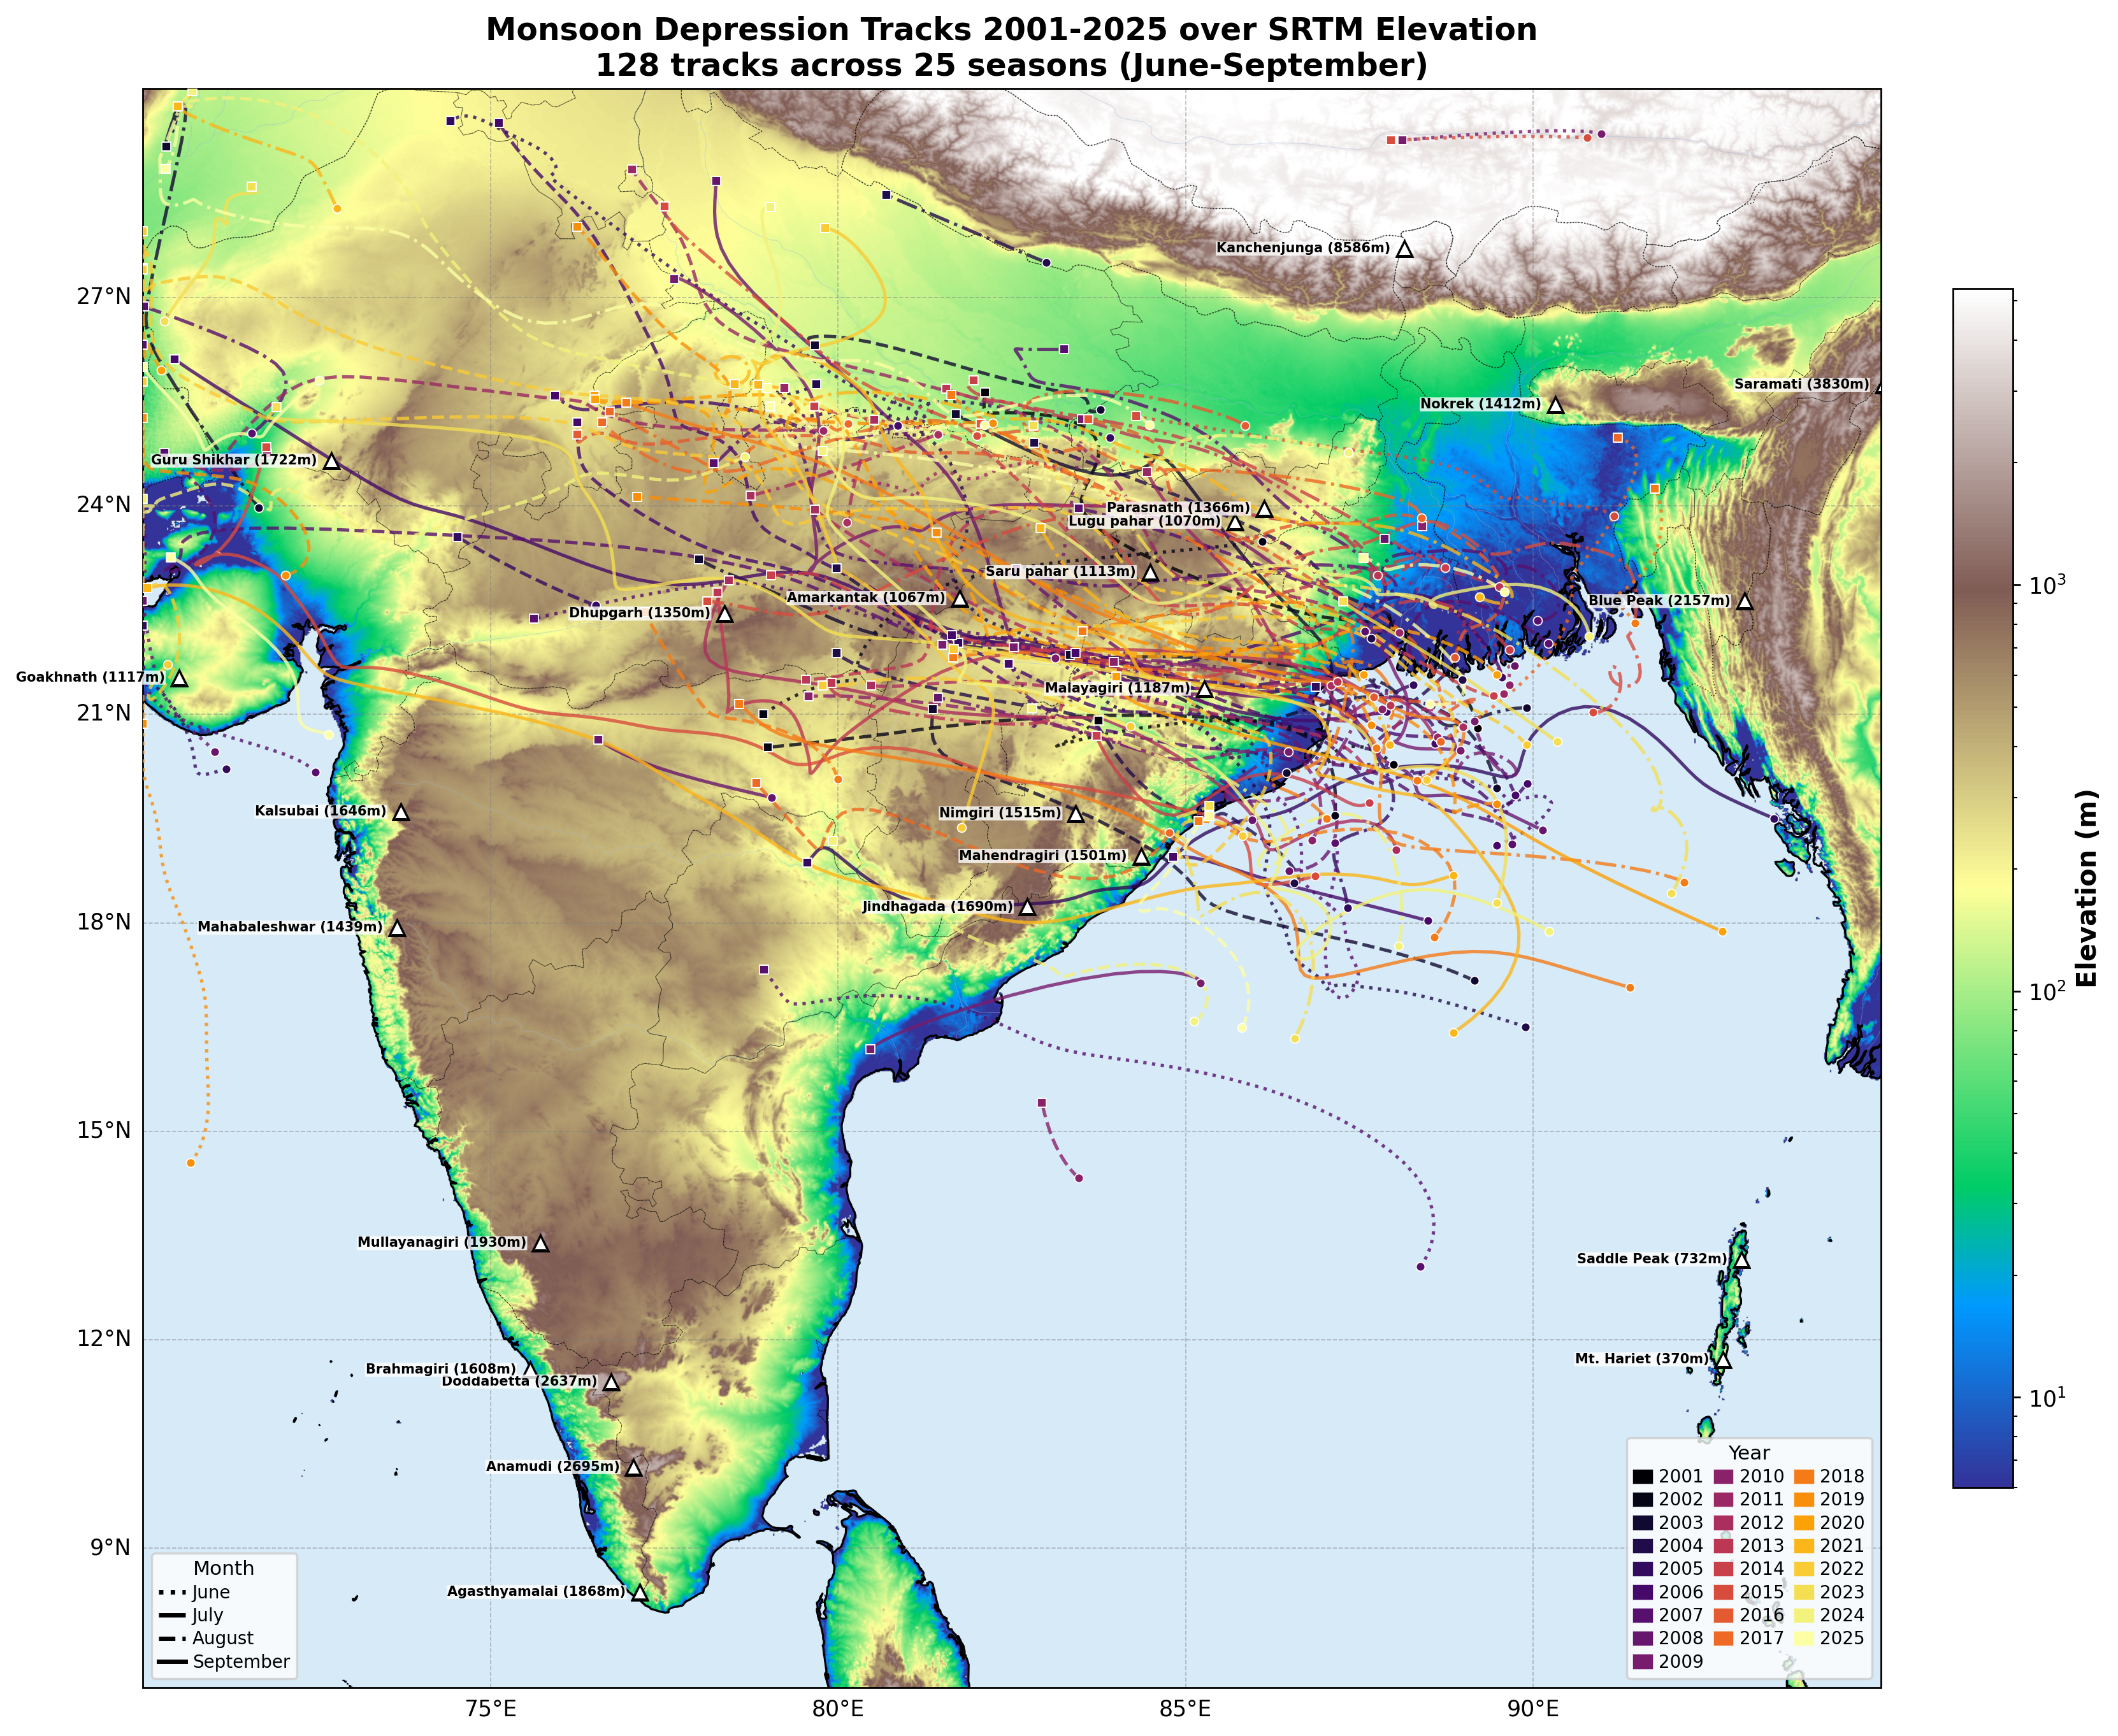
\includegraphics[width=0.95\textwidth]{all_years_tracks_elevation.png}
      \caption{\footnotesize All confirmed MD tracks (2001-2025)
      coloured by duration; Elevation from SRTM contours overlaid.}
    \end{figure}
  \end{columns}
\end{frame}
%
% ---------------------------------------------------------Slide:Interannual Trends
\setLayout{vertical}
\begin{frame}{Interannual Trends \& Duration Distribution}
  \begin{columns}
    \column{0.52\textwidth}
    \vspace{-1.1cm}
    \begin{figure}
      \centering
      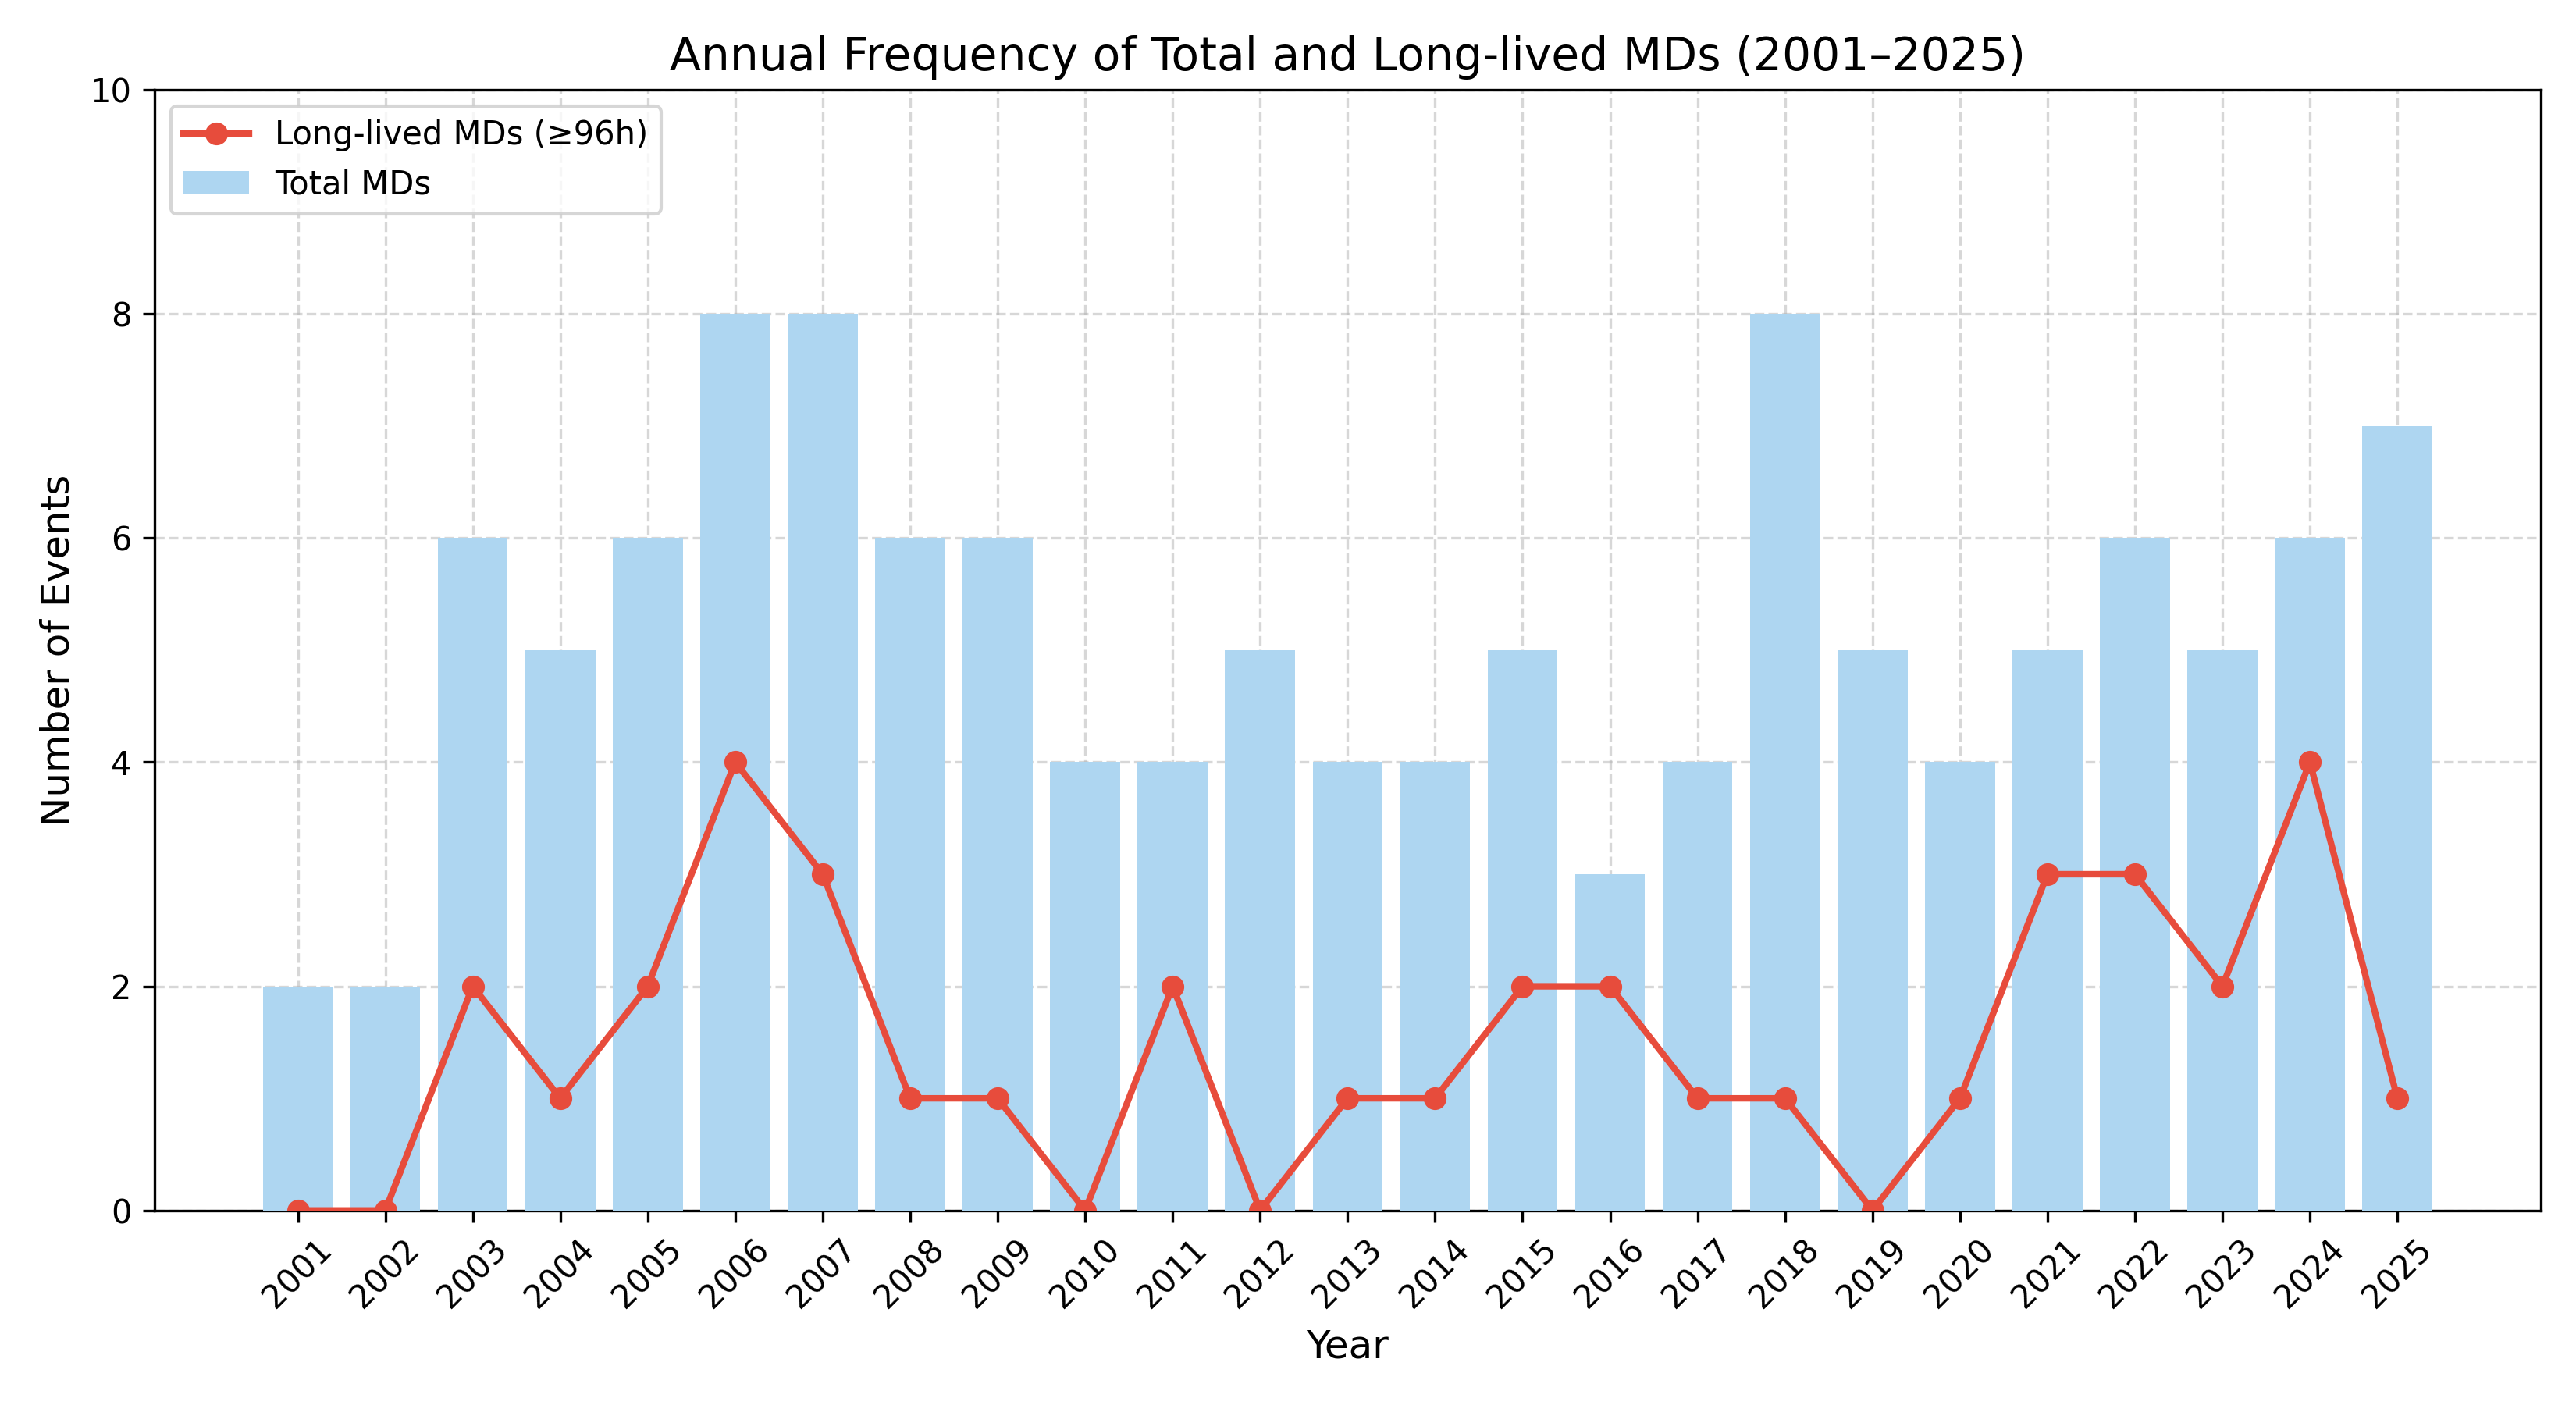
\includegraphics[width=\textwidth]{annual_count_trend}
      \caption{\footnotesize Annual MD frequency (bars) and
        long-lived system count (line), 2001-2025.}
        % Peak BOE years (2016, 2021, 2024) coincide with high antecedent soil moisture ($>0.35$ m$^3$\,m$^{-3}$).}
    \end{figure}

    \column{0.47\textwidth}
    \vspace{-1.1cm}
    \begin{figure}
      \centering
      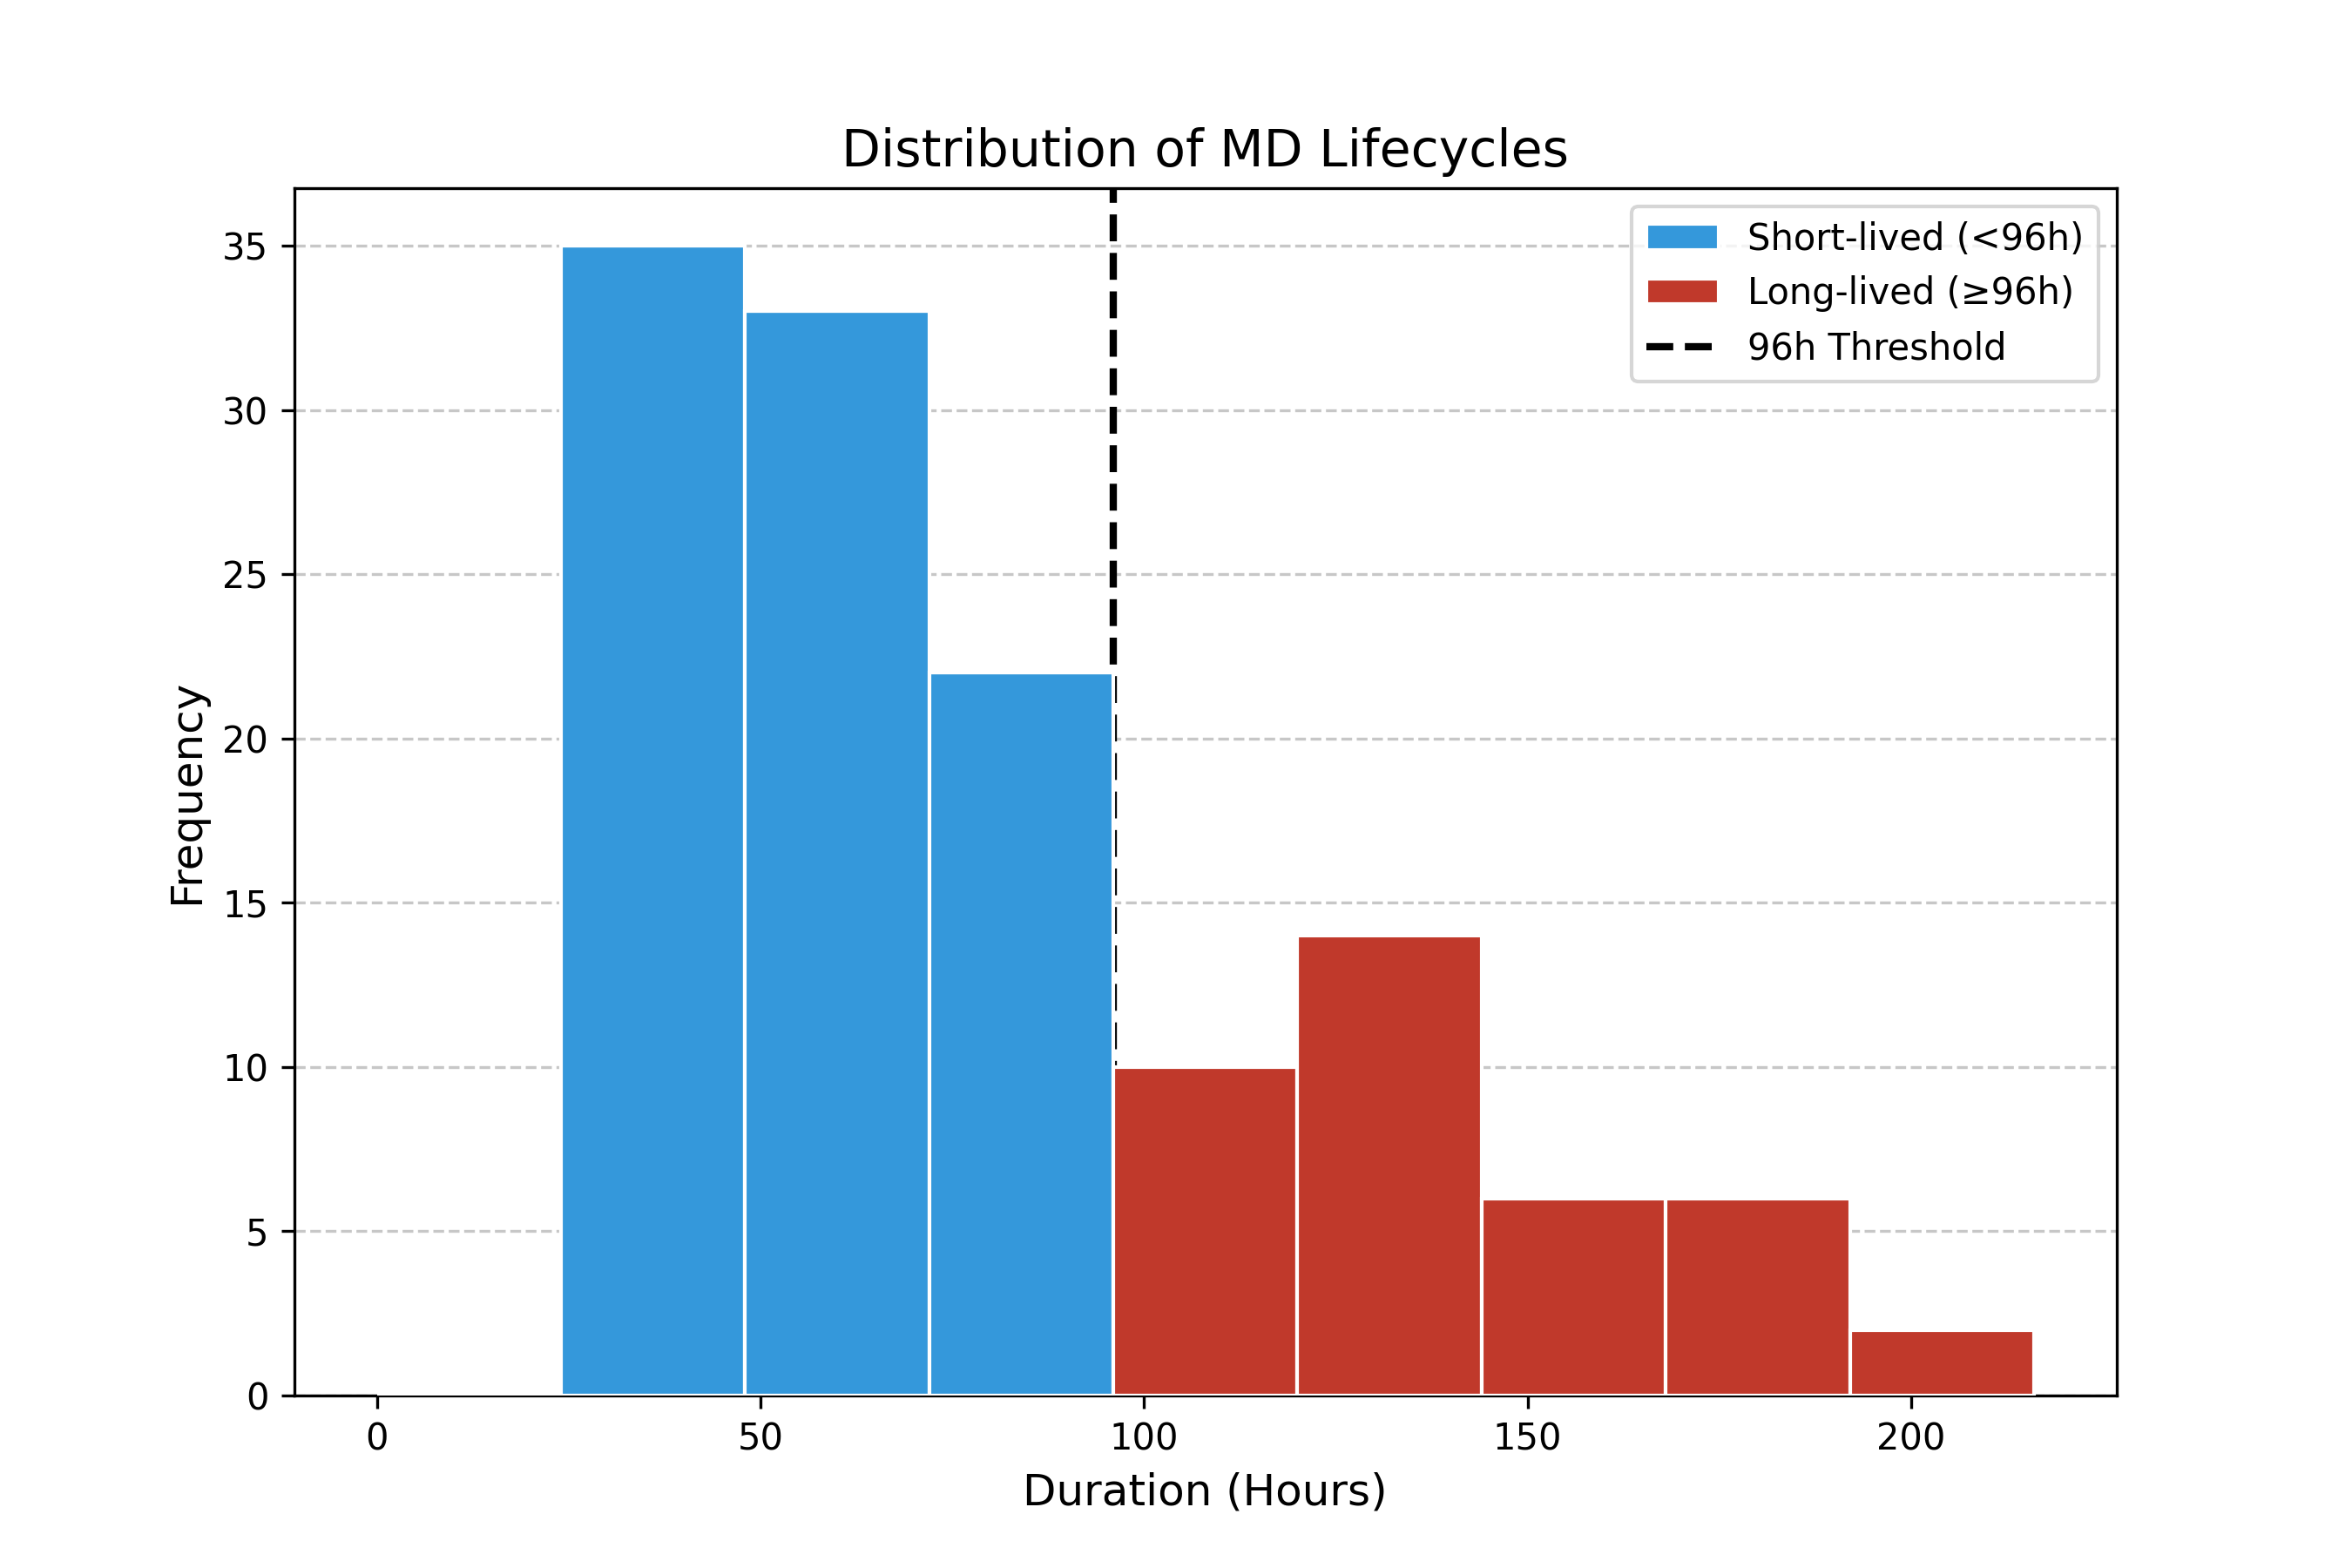
\includegraphics[width=0.90\textwidth]{duration_histogram}
      \caption{\footnotesize MD durations (24 h bins).
        Right-skewed distribution; the 96 h threshold separates
      short-lived (blue) from long-lived (red) populations.}
    \end{figure}
  \end{columns}

  \vspace{0.15cm}
  \scriptsize
  \begin{itemize}
    \item \textbf{Stable genesis:} Total annual count shows no
      significant trend ($p > 0.1$), consistent with Mishra (2021).
    \item \textbf{Variable longevity:} BOE candidate fraction
      varies dramatically year-to-year - controlled by land-surface
      moisture state, not genesis frequency.
  \end{itemize}
\end{frame}

% SECTION III - PROCESS-LEVEL RESULTS
\section{Process-Level Results}
\setLayout{mainpoint}
\begin{frame}{}
  \frametitle{RESULTS: AZIMUTHAL HOVMÖLLER ANALYSIS}
\end{frame}

%---------------------------------------------------------Slide: Representative Cases
\setLayout{plain}
\begin{frame}{Cases: BOE vs. Non-BOE Systems}
  \begin{columns}
    \column{0.50\textwidth}
    \vspace{-1.1cm}
    \begin{figure}
      \centering
      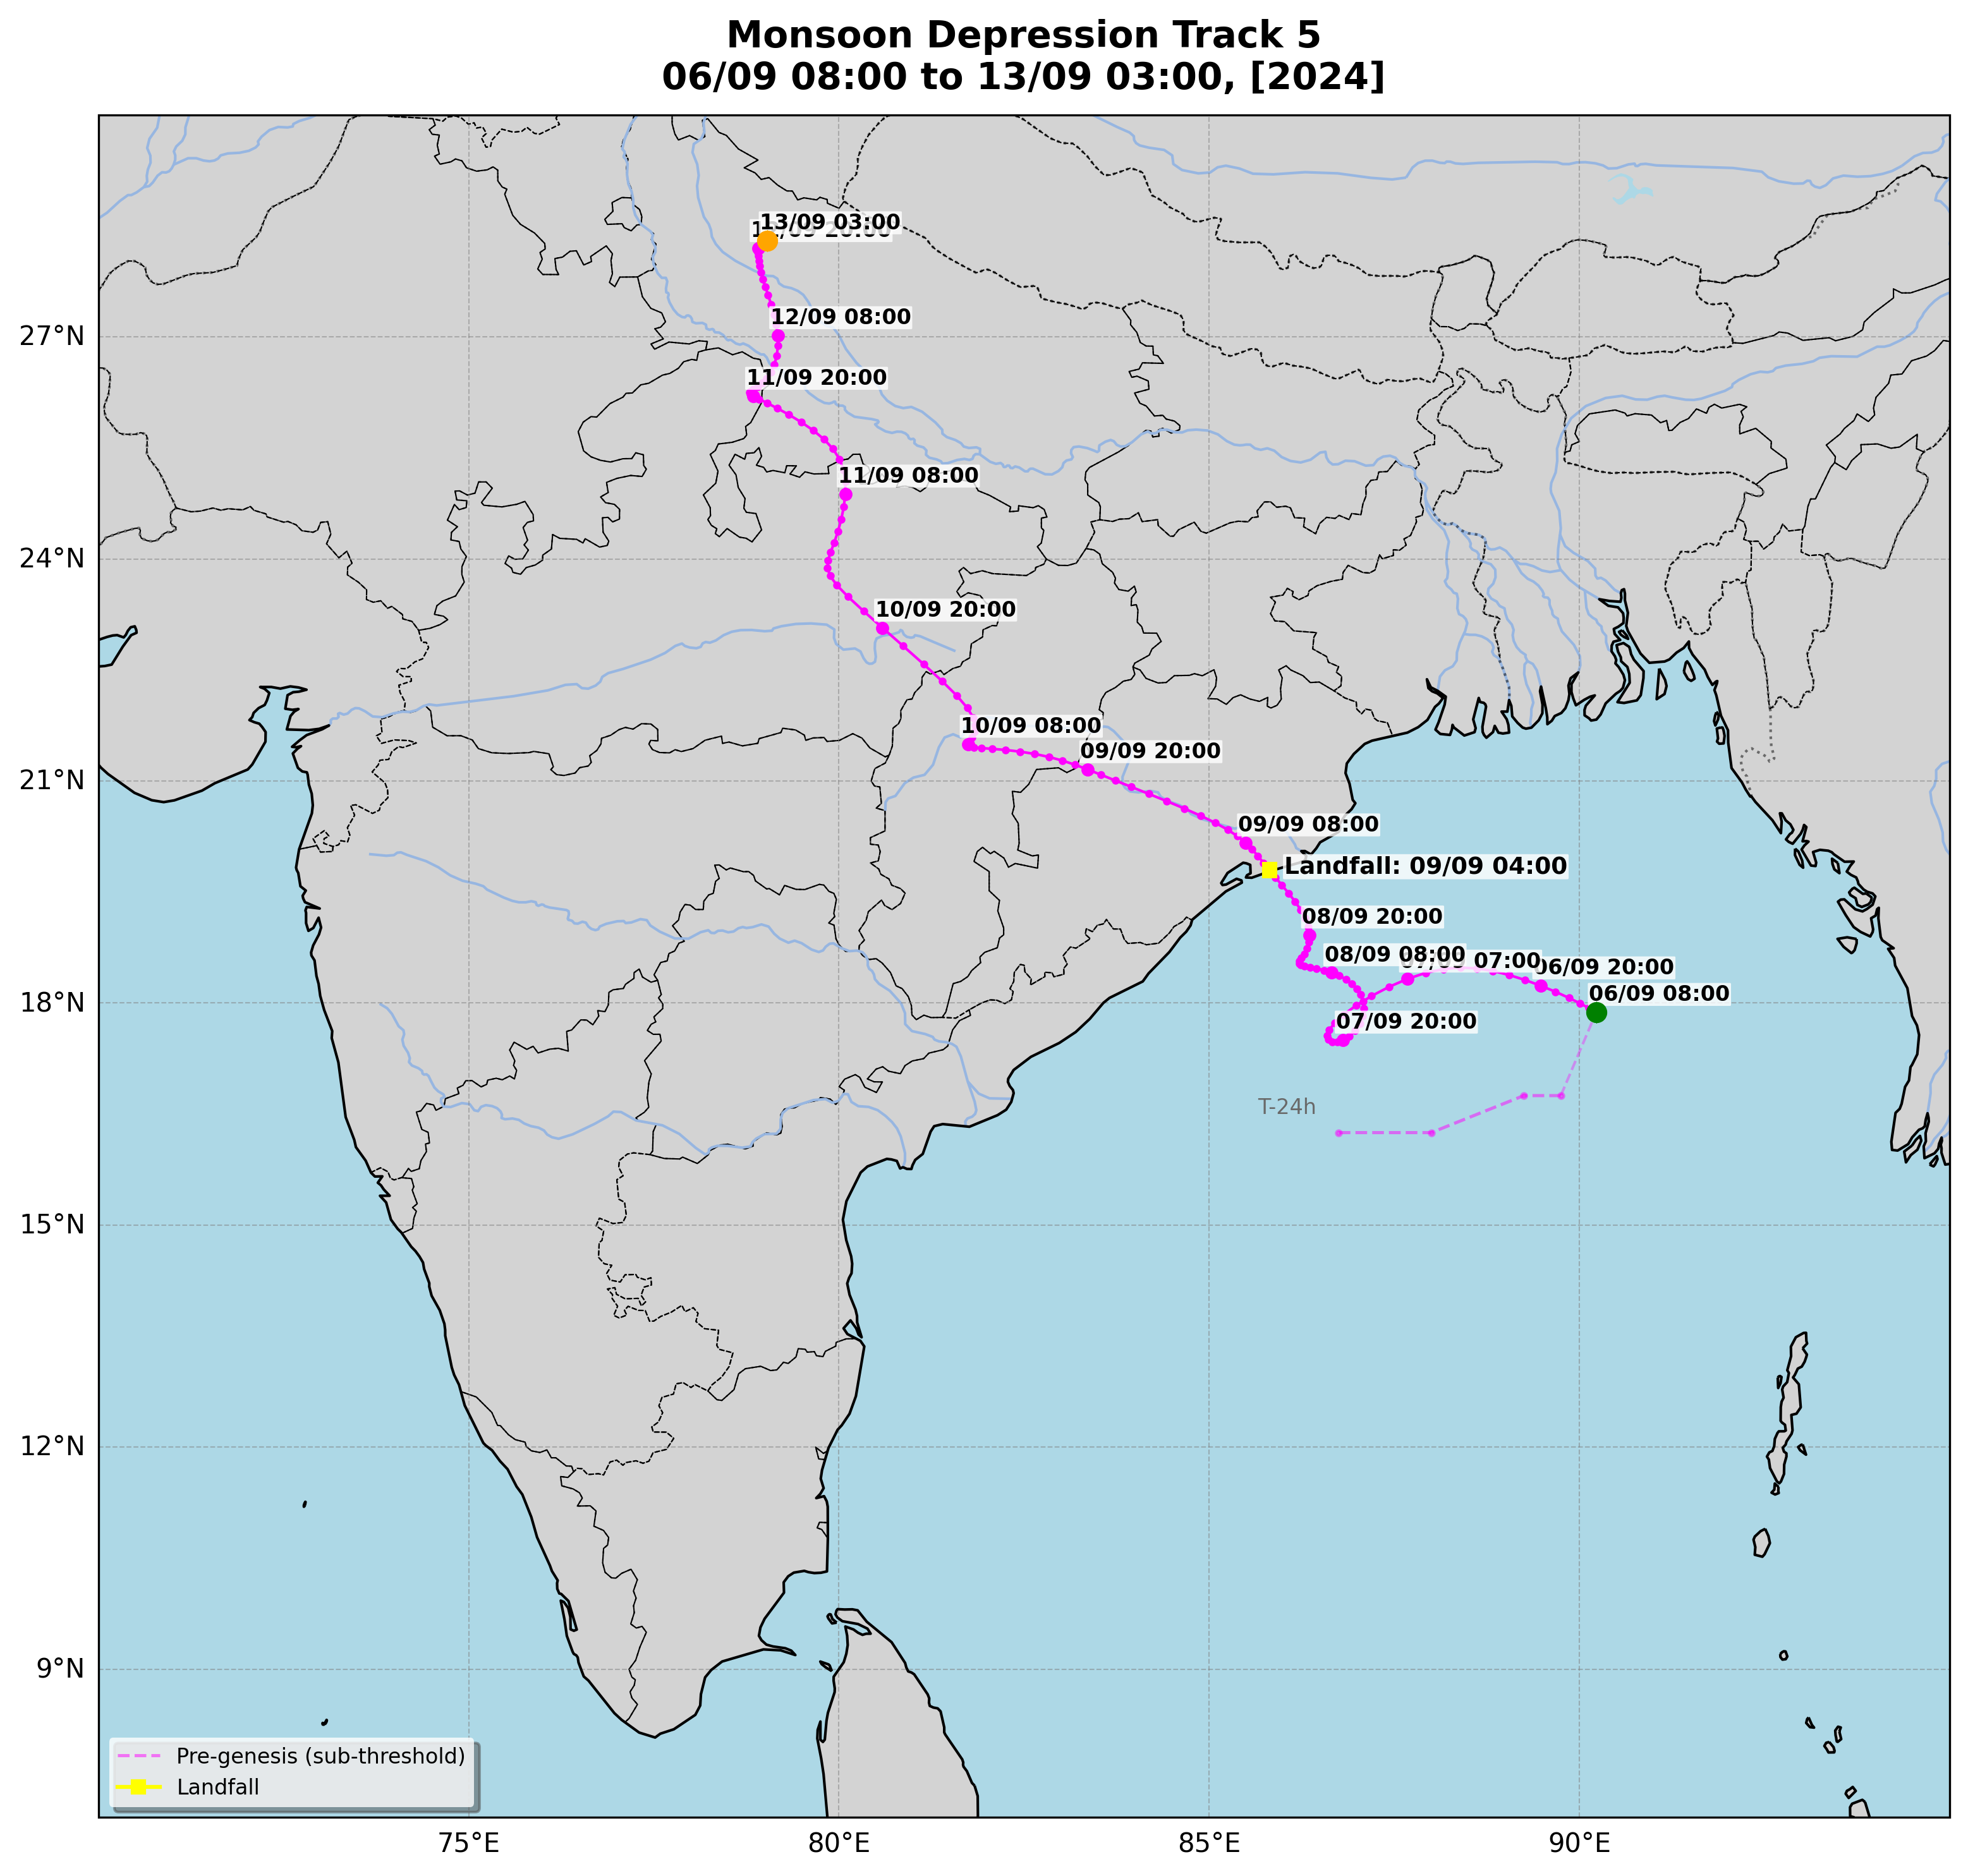
\includegraphics[width=0.8\textwidth]{track_long_spatial}
      \caption{\scriptsize \textbf{BOE-Active (Long-lived):}
        September 2024 system - sustained westward trajectory, crosses
      Eastern Ghats, penetrates deep into the Indian heartland.}
    \end{figure}

    \column{0.50\textwidth}
    \vspace{-1.1cm}
    \begin{figure}
      \centering
      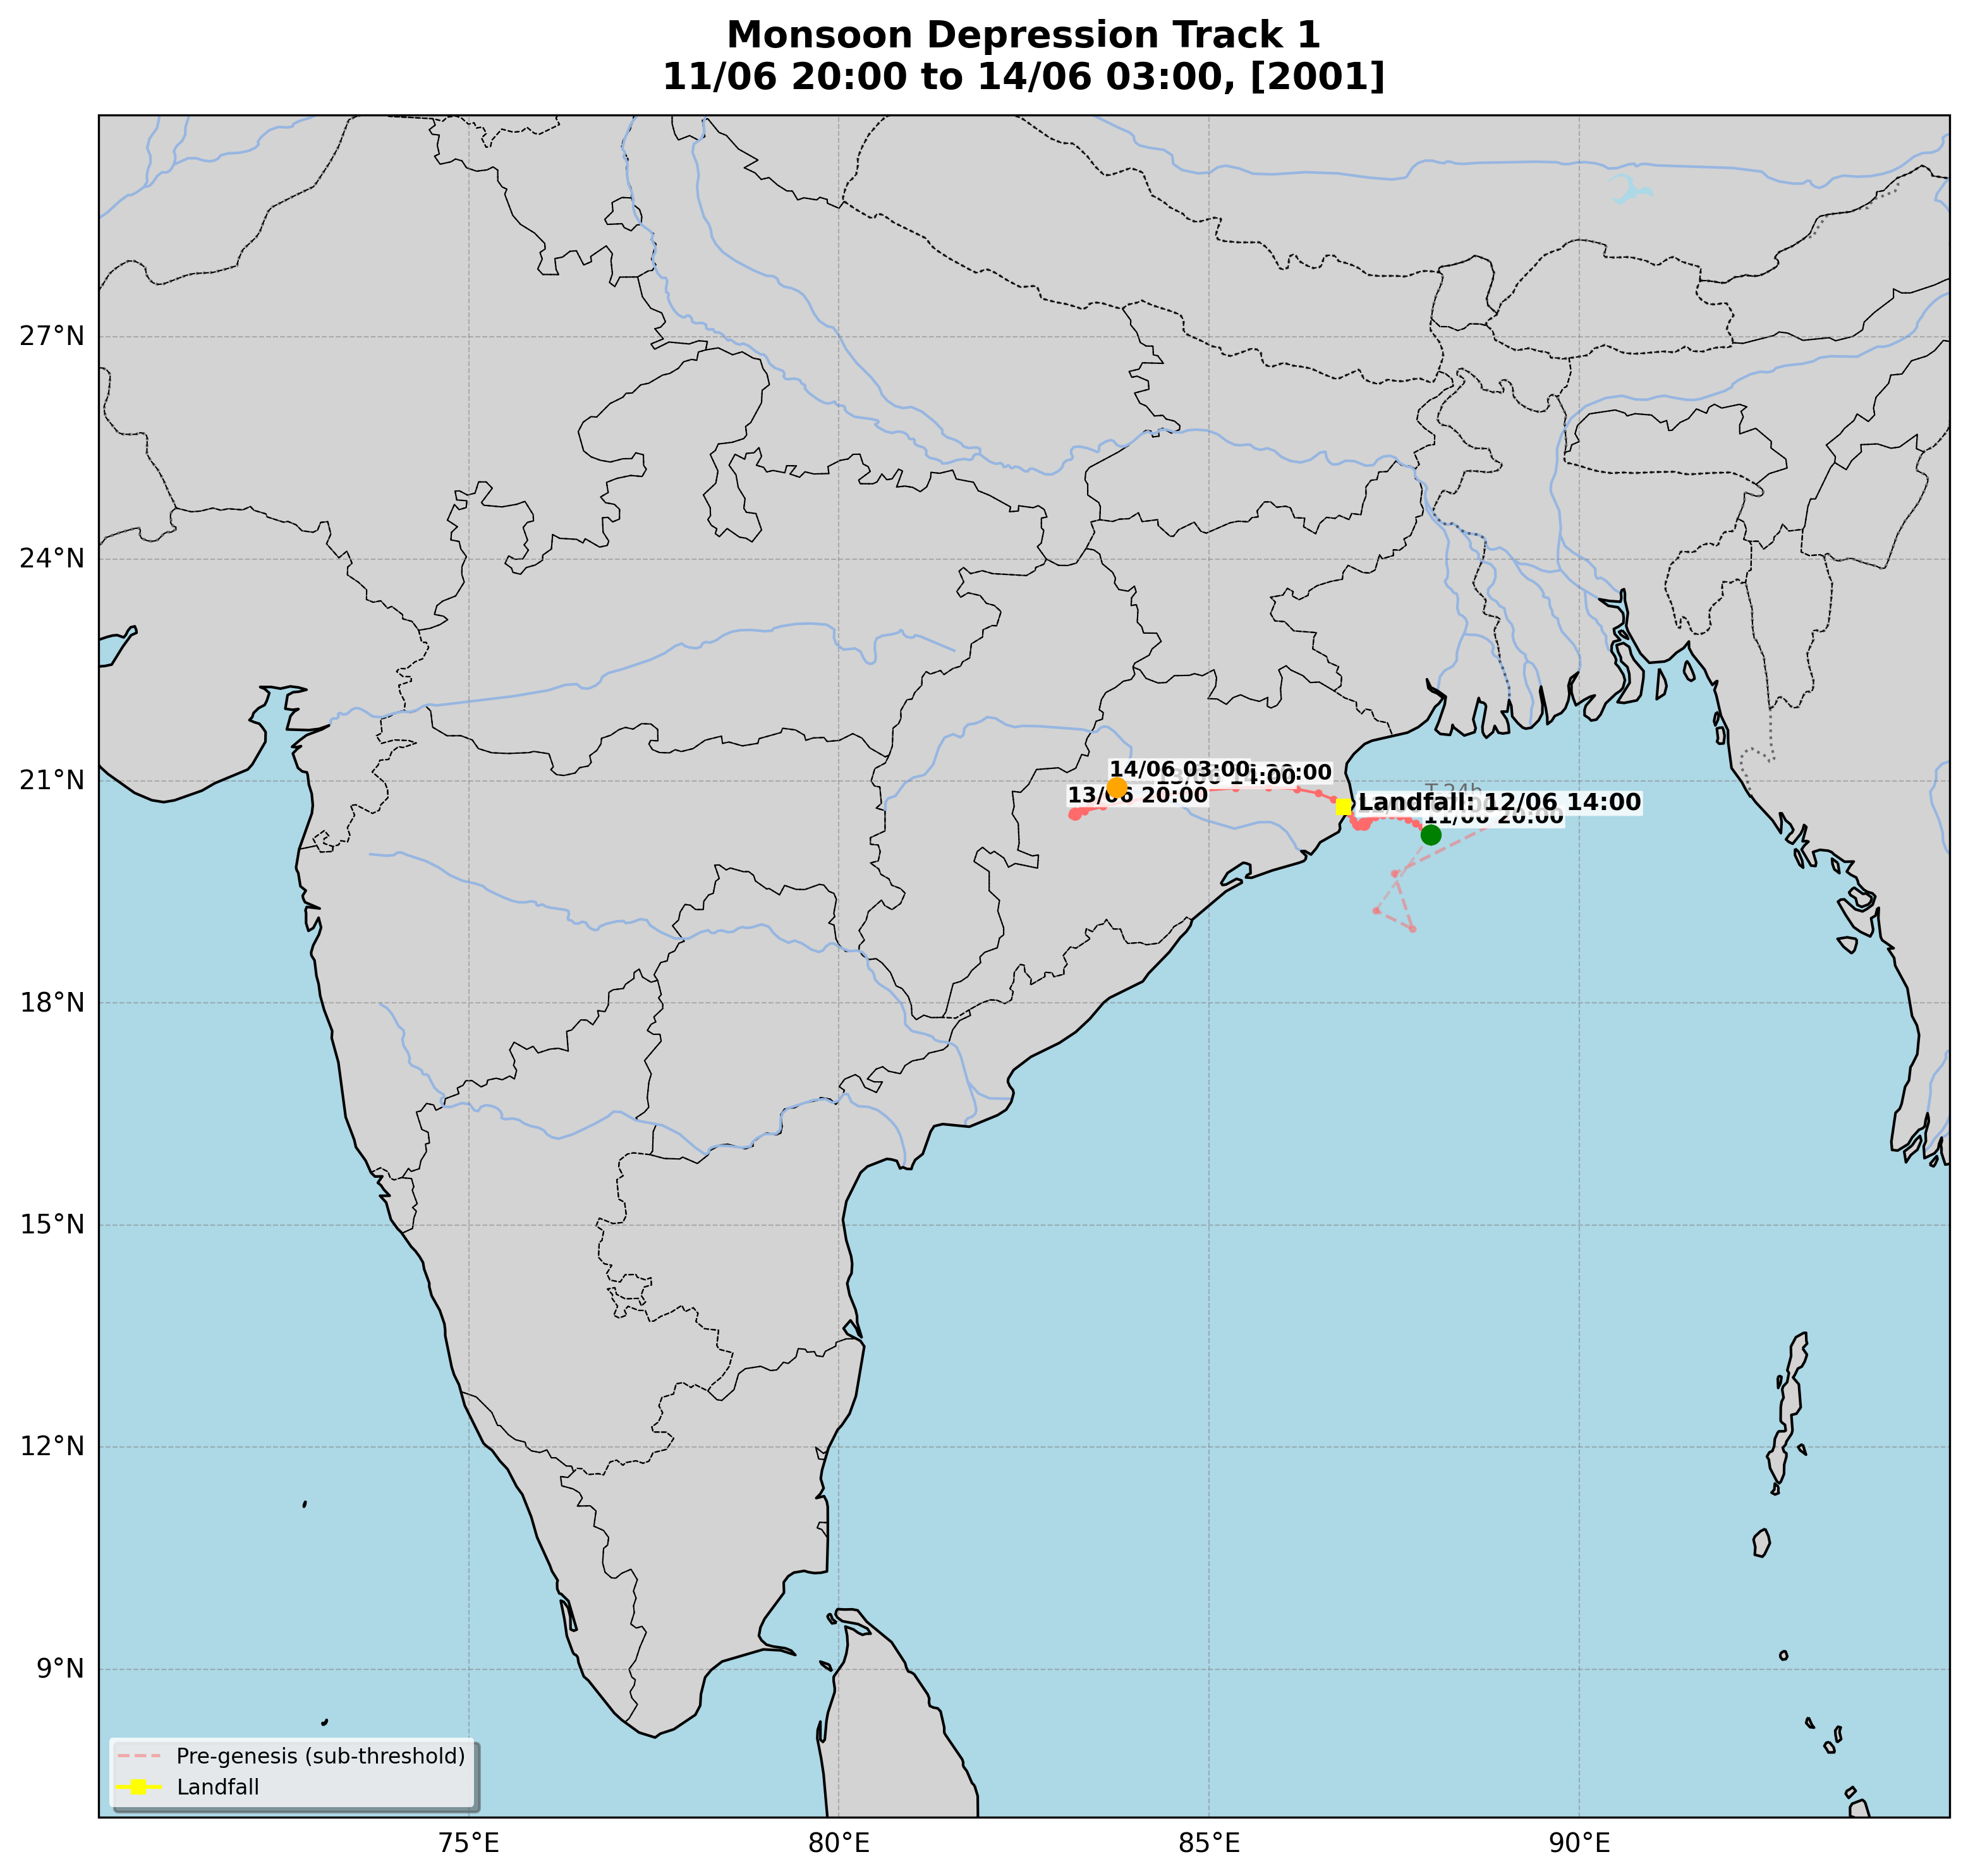
\includegraphics[width=0.8\textwidth]{track_short_spatial}
      \caption{\scriptsize \textbf{Non-BOE (Short-lived):} June
        2001 system - terminates on the windward slopes of the Eastern
      Ghats within 48 h of landfall.}
    \end{figure}
  \end{columns}

  \vspace{-0.1cm}
  \footnotesize
  These two tracks serve as the representative pair for the
  Hovmöller analysis. The BOE case meets the $\geq 70$ W m$^{-2}$ LHF
  criterion for $>72$ h; the non-BOE case fails within 36 h of landfall.
\end{frame}

%---------------------------------------------------------Slide:
% Precipitation Dynamics
\setLayout{plain}
\begin{frame}{Precipitation Dynamics: Structural Regime Shift at Landfall}
  \begin{columns}
    \column{0.50\textwidth}
    \vspace{-1.1cm}
    \begin{figure}
      \centering
      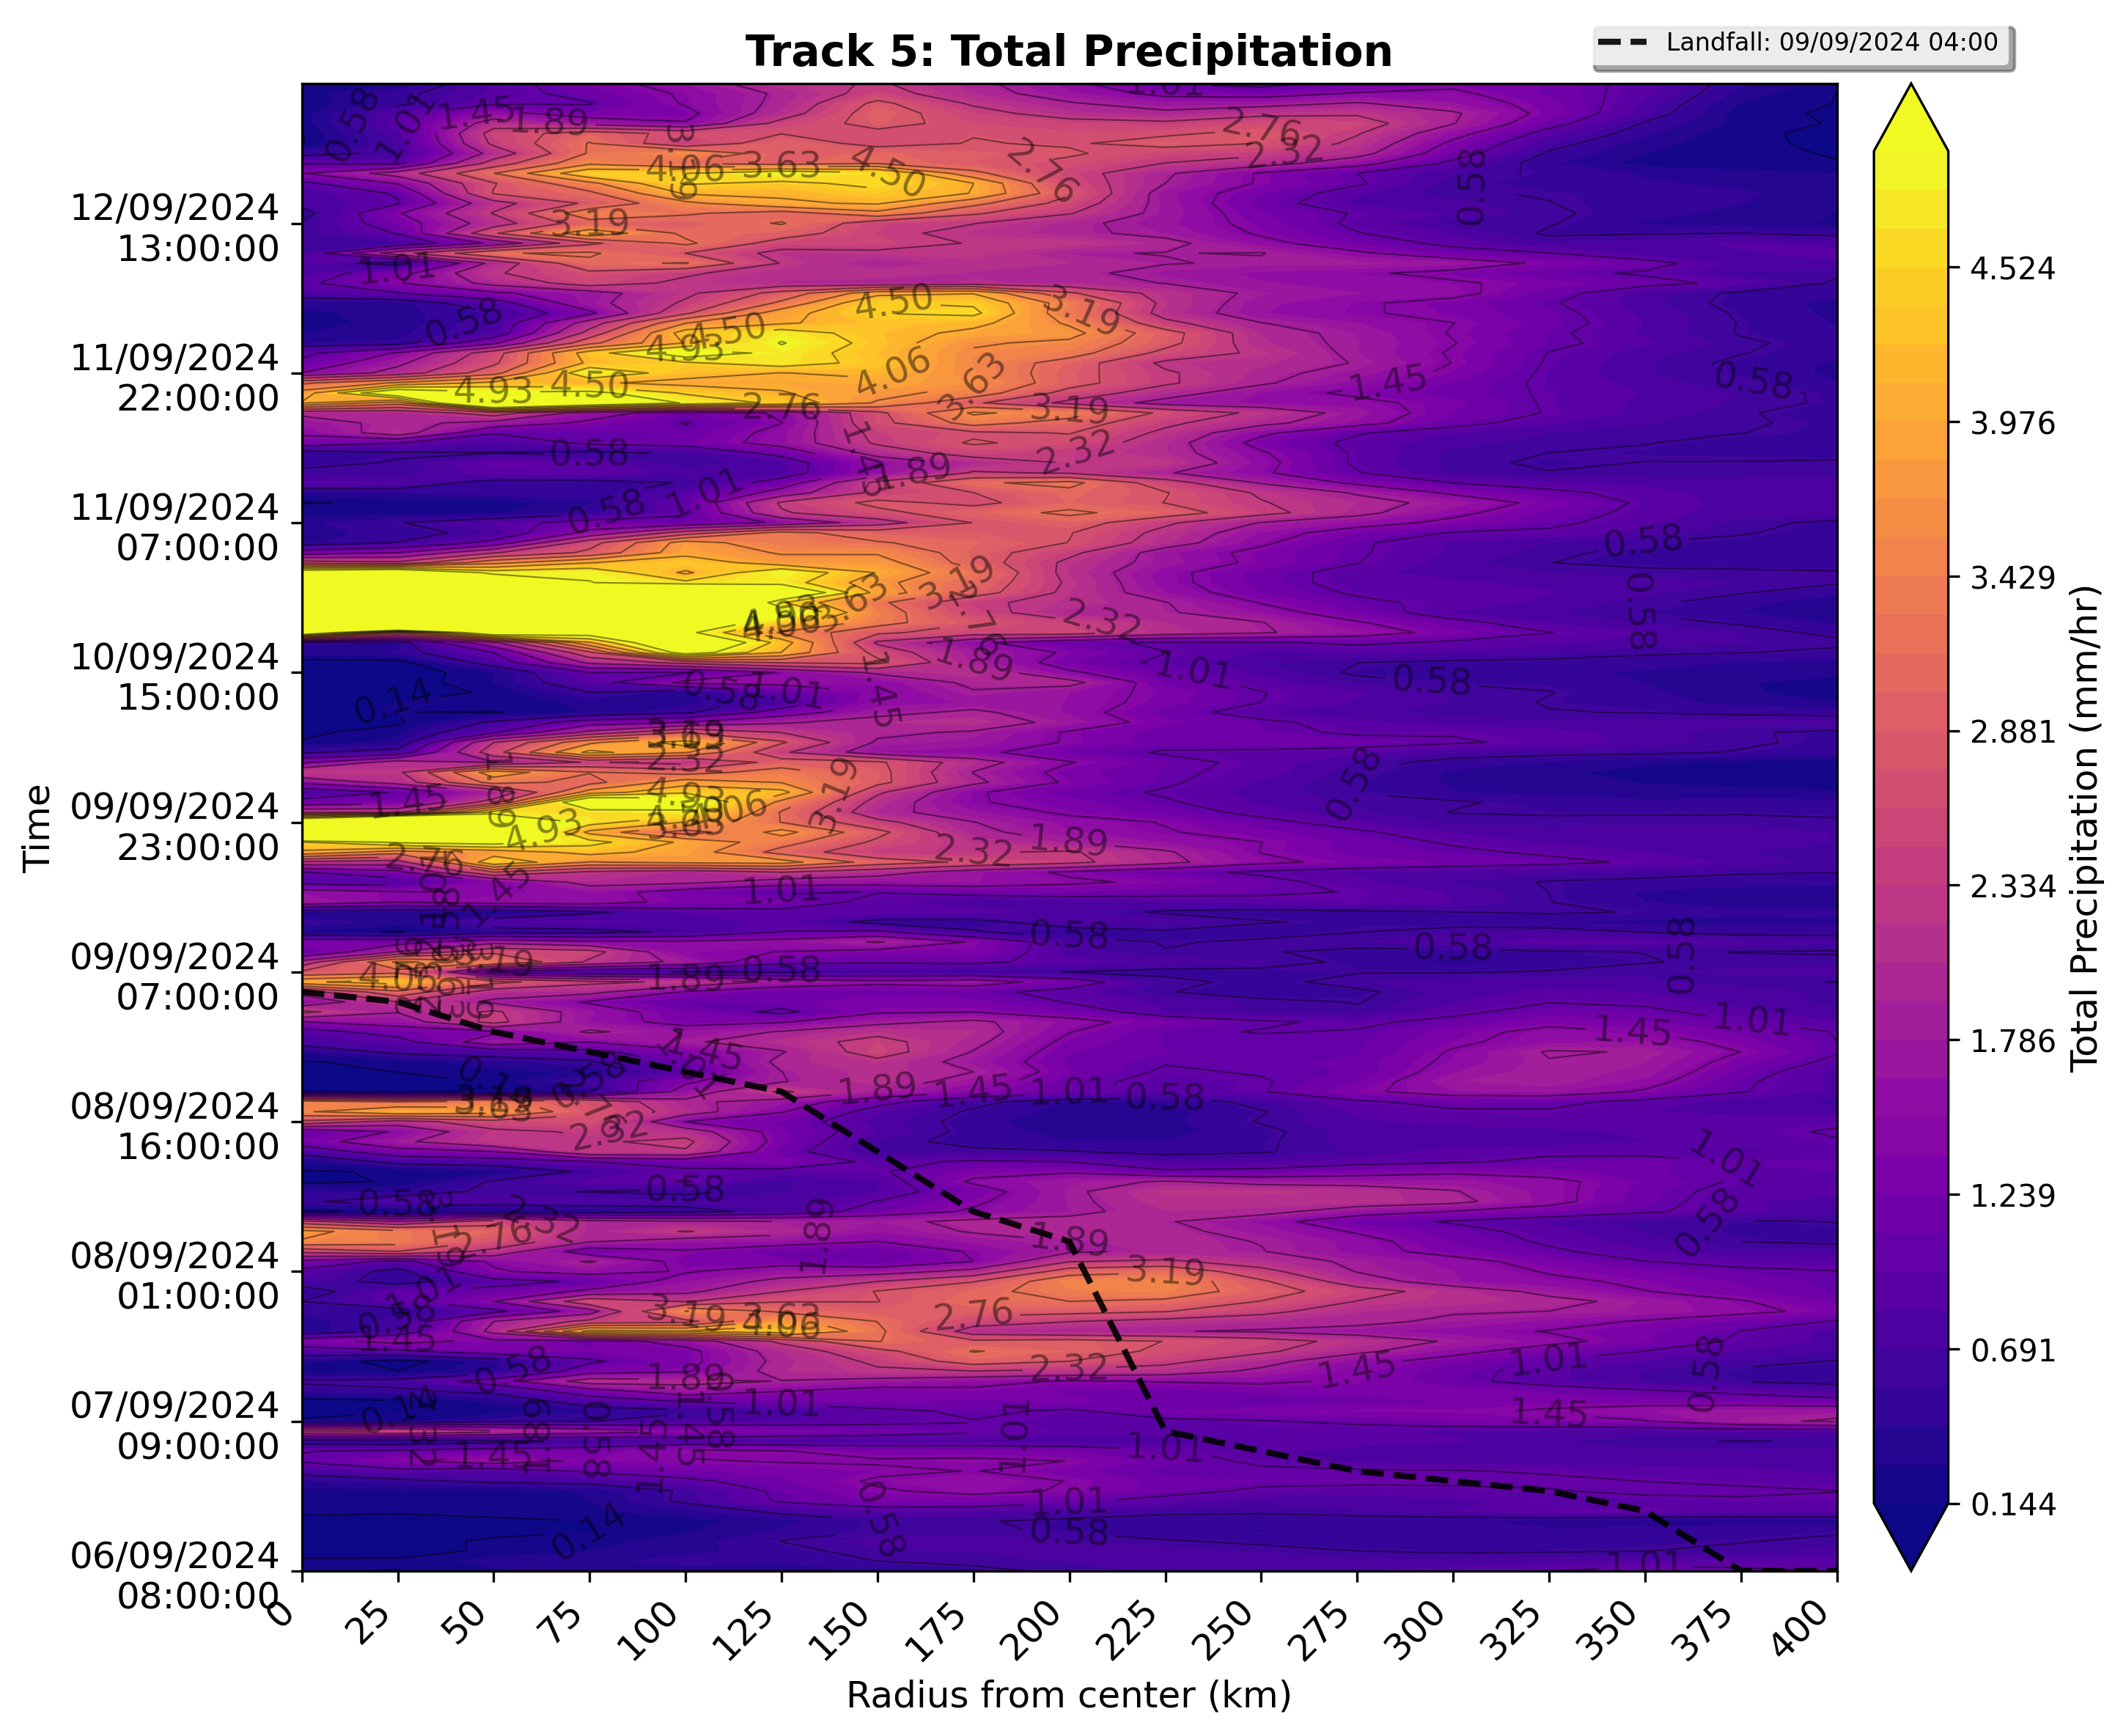
\includegraphics[width=0.92\textwidth]{track_long_tp_hov}
      \caption{\scriptsize \textbf{BOE-Active:} Precipitation
        contracts to inner core ($<100$ km) post-landfall. Self-wetting
      feedback sustains uniform inner-core precipitation.}
    \end{figure}

    \column{0.50\textwidth}
    \vspace{-1.1cm}
    \begin{figure}
      \centering
      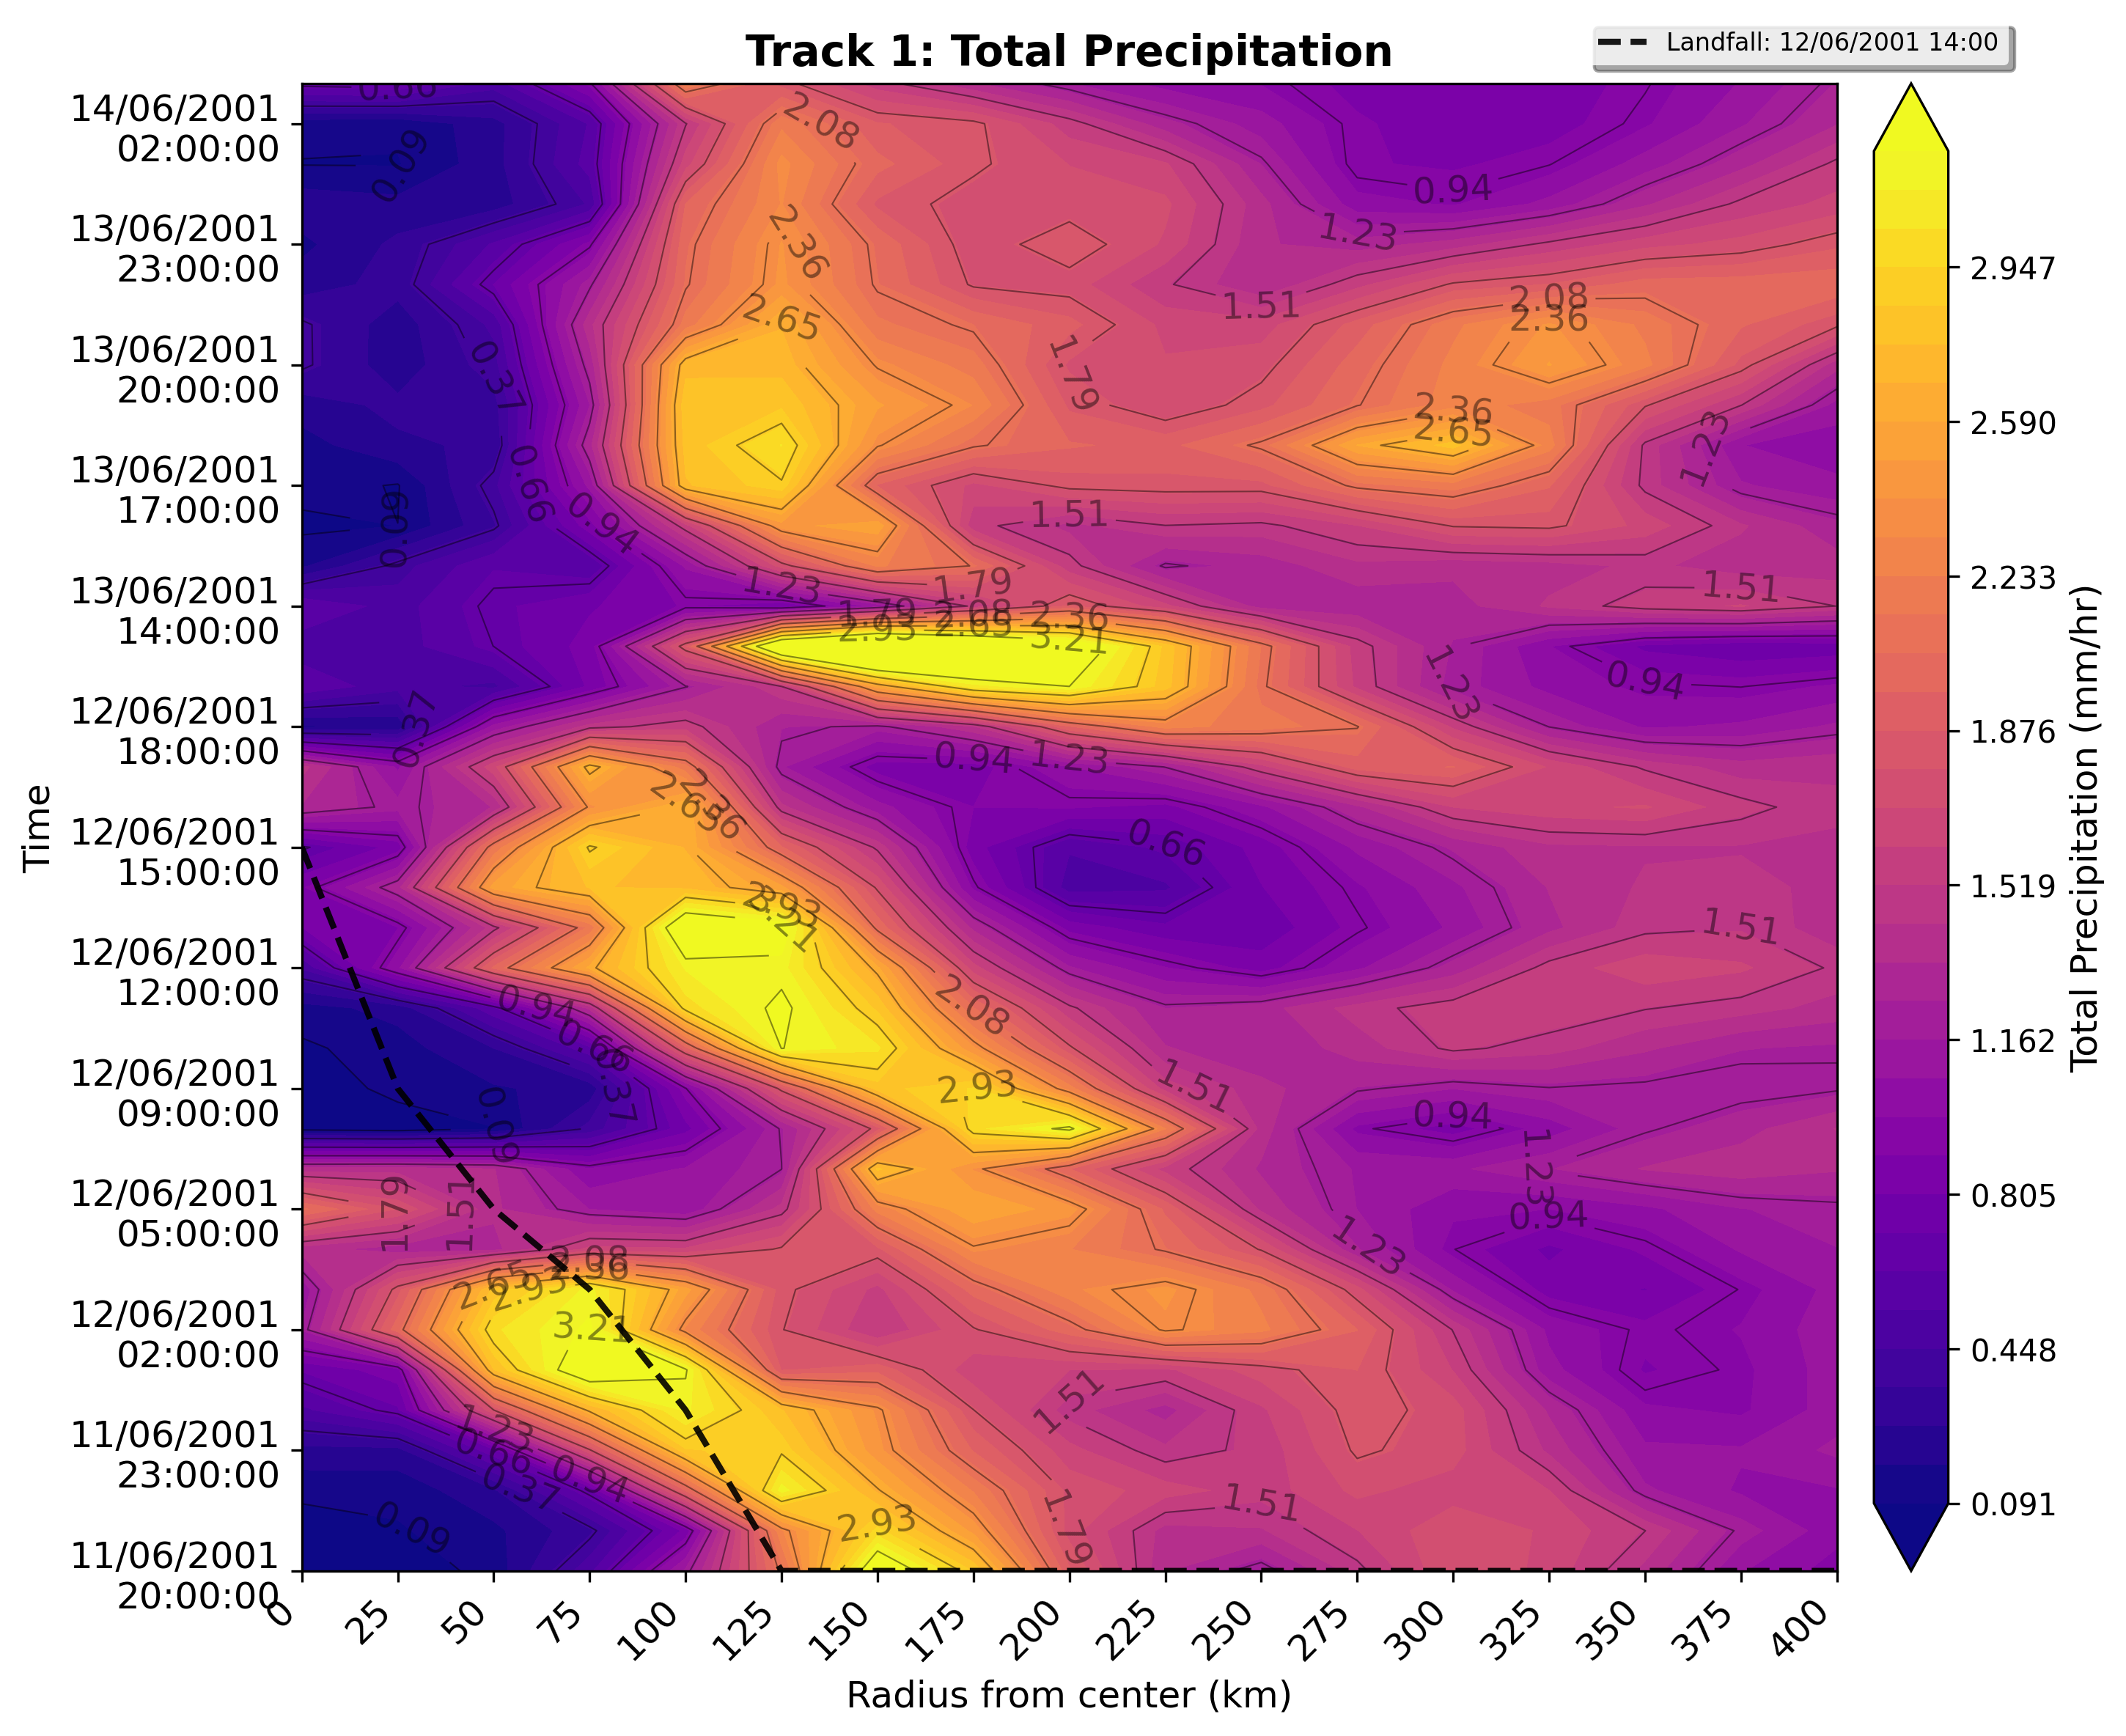
\includegraphics[width=0.92\textwidth]{track_short_tp_hov}
      \caption{\scriptsize \textbf{Non-BOE:} Heavy precipitation
        at landfall followed by simultaneous collapse of both core and
      peripheral convection within 24 h.}
    \end{figure}
  \end{columns}

  \vspace{-0.15cm}
  \footnotesize
  The BOE system shifts from broad maritime rainbands to a
  self-sustaining contracted inner core. The non-BOE system's outer
  convection dies quickly as the land surface becomes energy-limited.
\end{frame}

%---------------------------------------------------------Slide: Soil Moisture
\setLayout{plain}
\begin{frame}{Soil Moisture: Important for MD Longevity}
  \begin{columns}
    \column{0.50\textwidth}
    \vspace{-1.2cm}
    \begin{figure}
      \centering
      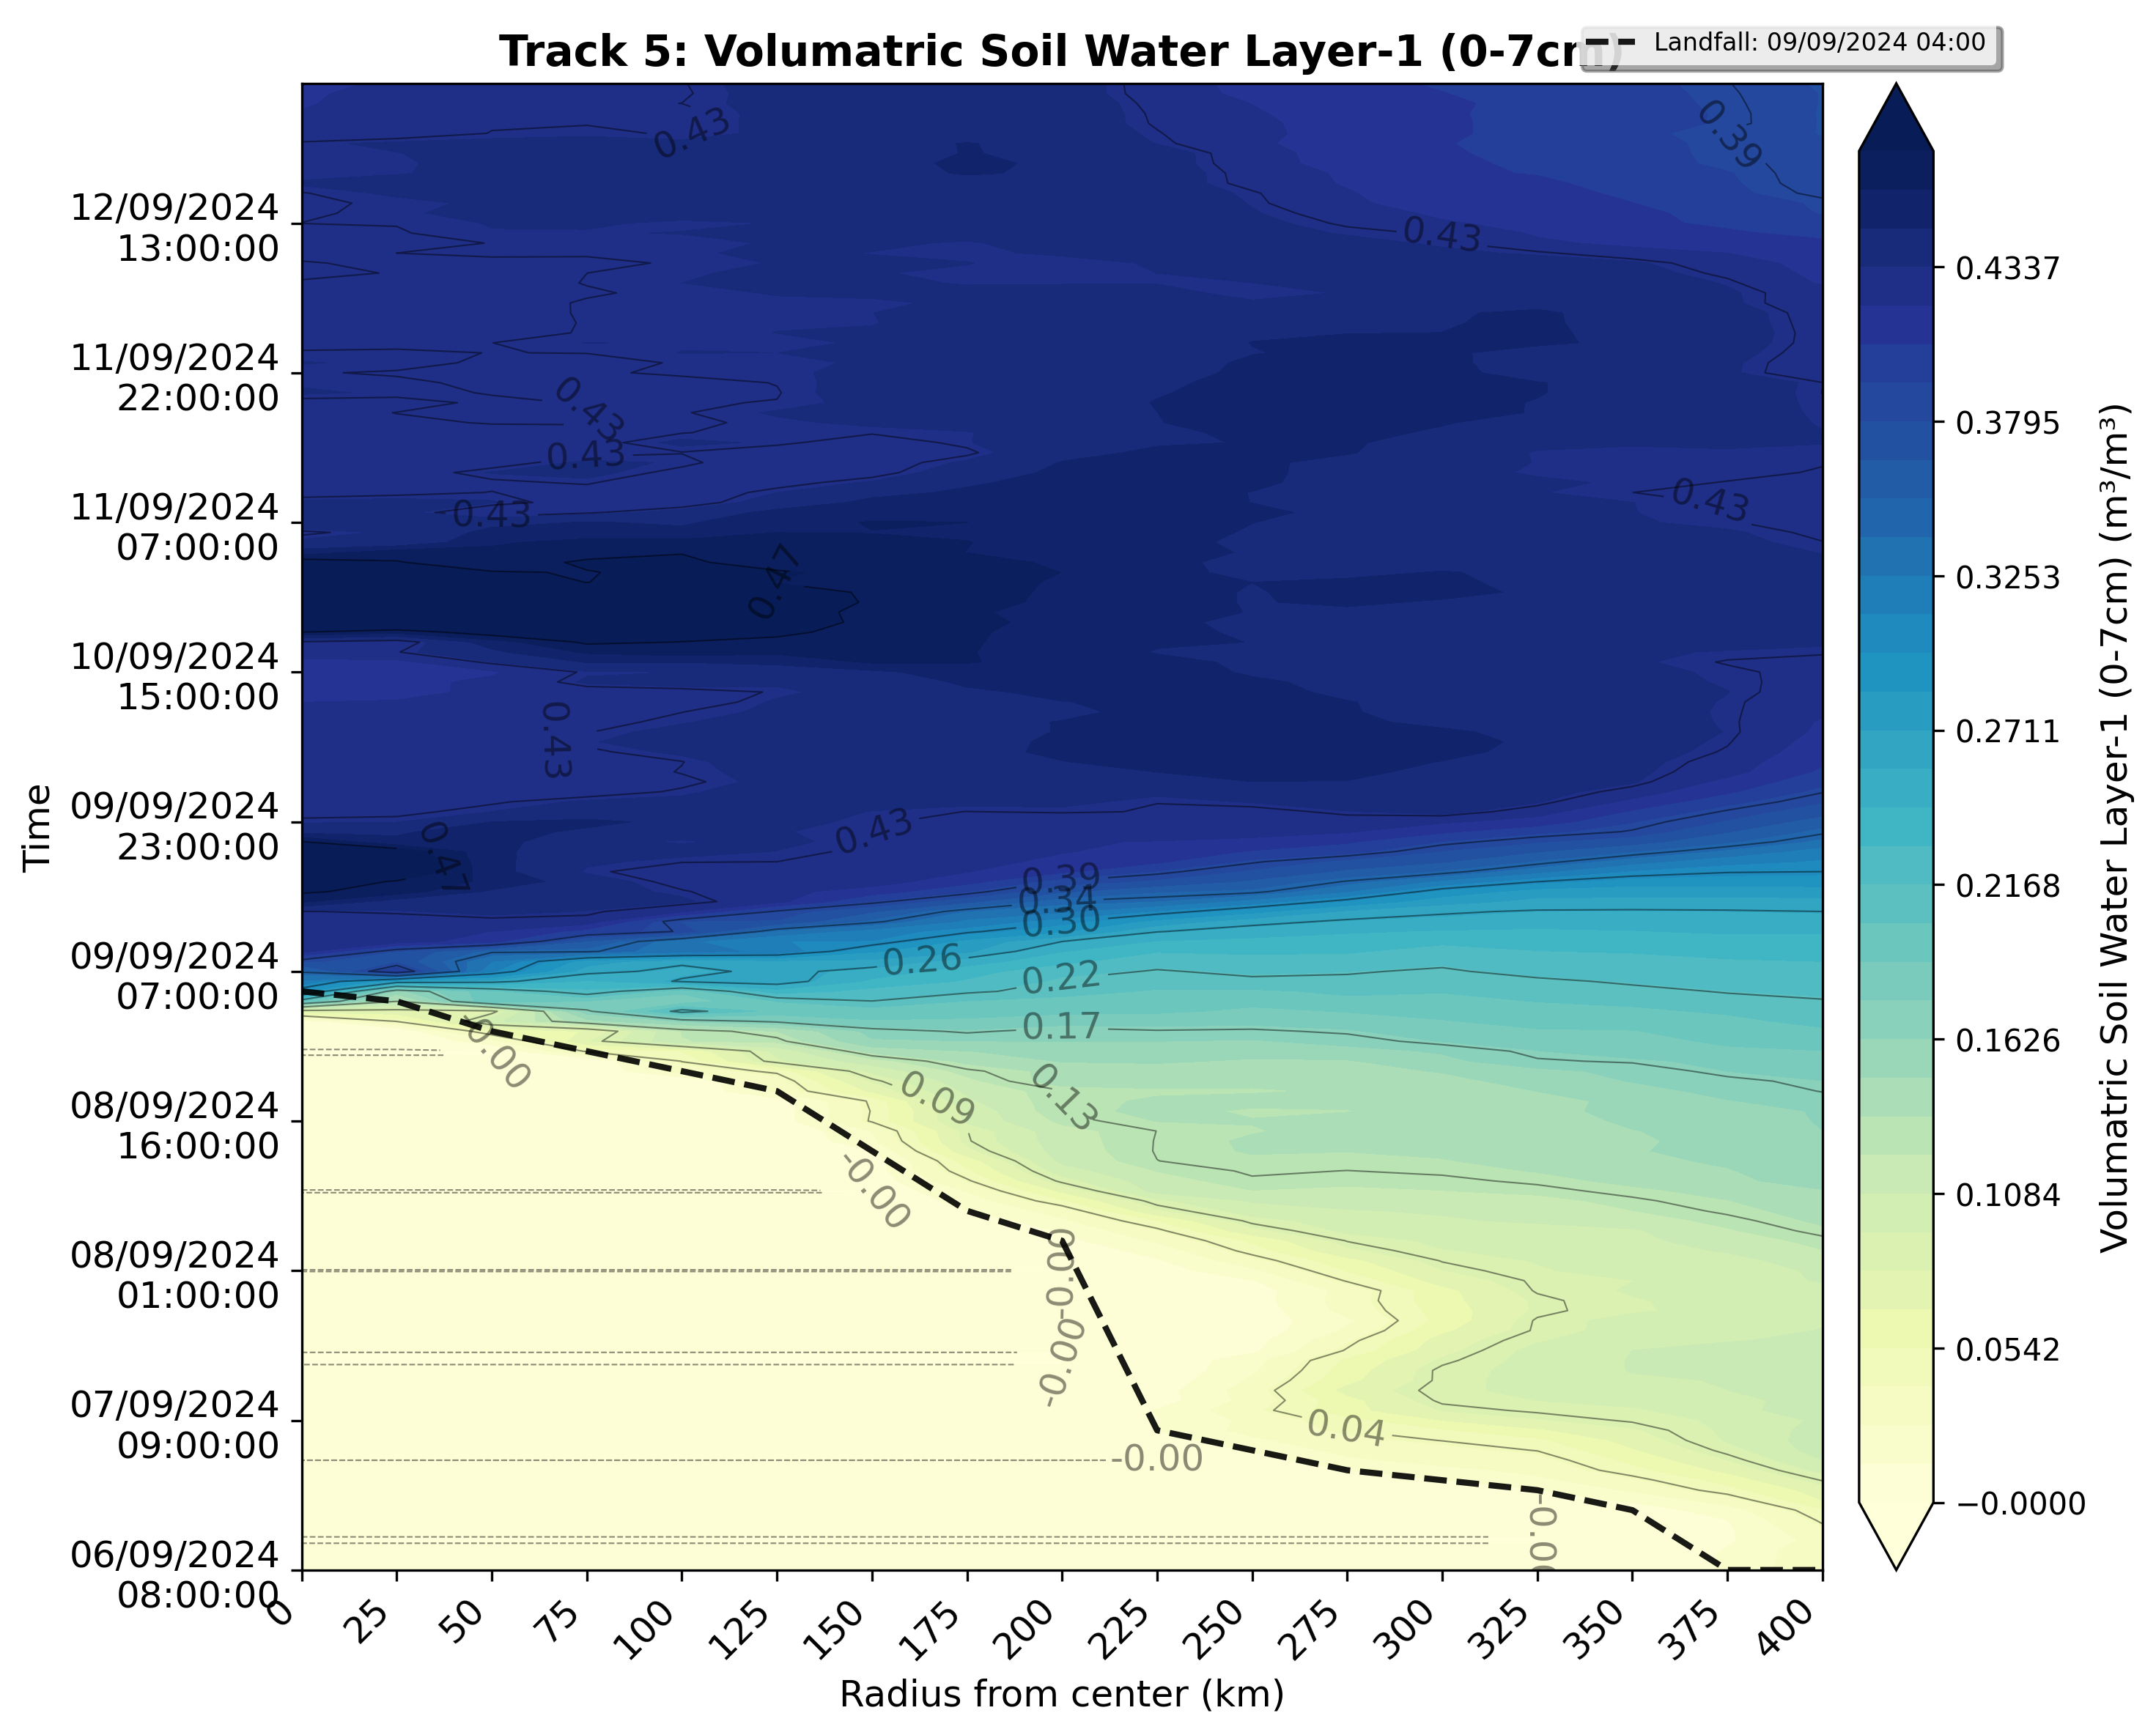
\includegraphics[width=0.90\textwidth]{track_long_swvl1_hov}
      \caption{\scriptsize \textbf{BOE-Active:} Sustained
        exposure to high SWVL1 ($\gtrsim 0.38$ m$^3$\,m$^{-3}$) for $>72$ h
        post-landfall. Self-wetting signal: widening saturated core at
      $r < 100$ km.}
    \end{figure}

    \column{0.50\textwidth}
    \vspace{-1.2cm}
    \begin{figure}
      \centering
      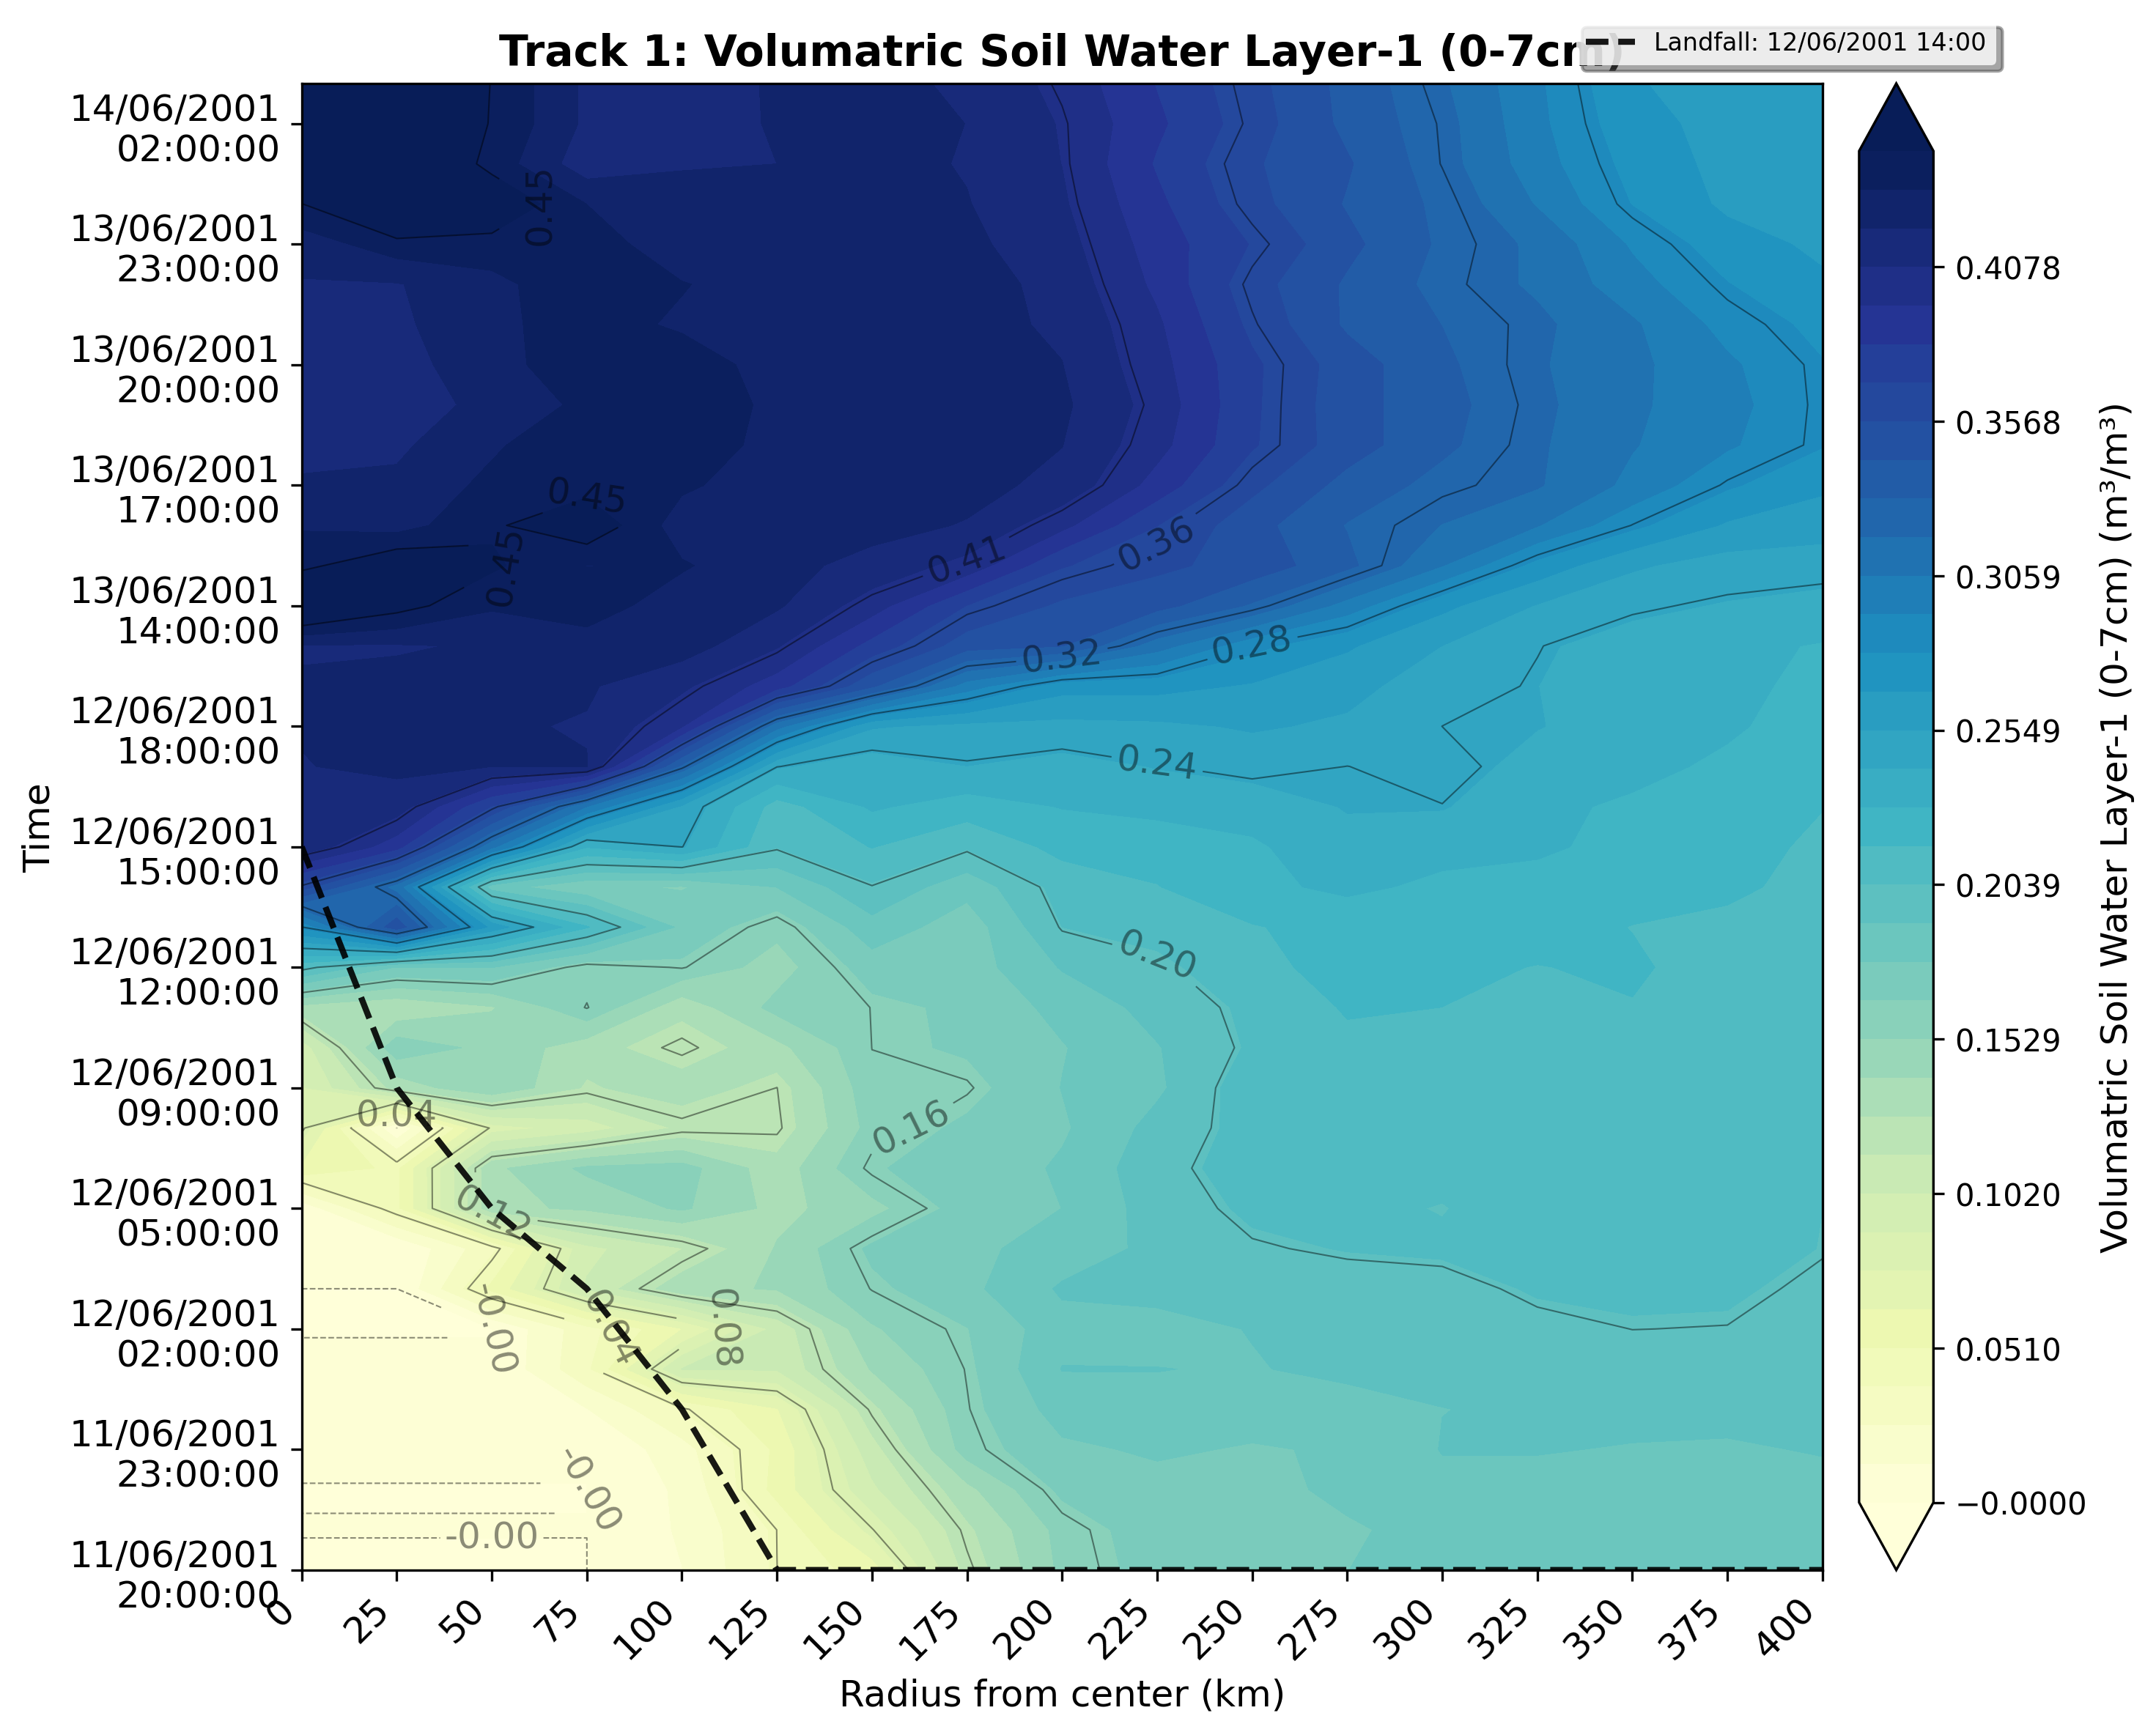
\includegraphics[width=0.90\textwidth]{track_short_swvl1_hov}
      \caption{\scriptsize \textbf{Non-BOE:} Initial soil
        moisture may be similar, but exposure duration is severely
      truncated. Rapid surface desiccation cuts the energy supply.}
    \end{figure}
  \end{columns}

  \vspace{-0.15cm}
  \scriptsize
  Persistence of moist surface contact, not just initial soil
  moisture, is the reason for MD longevity. Both systems may
  encounter moist soils at landfall, but only BOE-active systems
  maintain this contact through the self-wetting loop.
\end{frame}

%---------------------------------------------------------Slide:
% LHF - The BOE Energy Signal
\setLayout{plain}
\begin{frame}{Latent Heat Flux: The BOE Energy Signal}
  \begin{columns}
    \column{0.50\textwidth}
    \vspace{-1.22cm}
    \begin{figure}
      \centering
      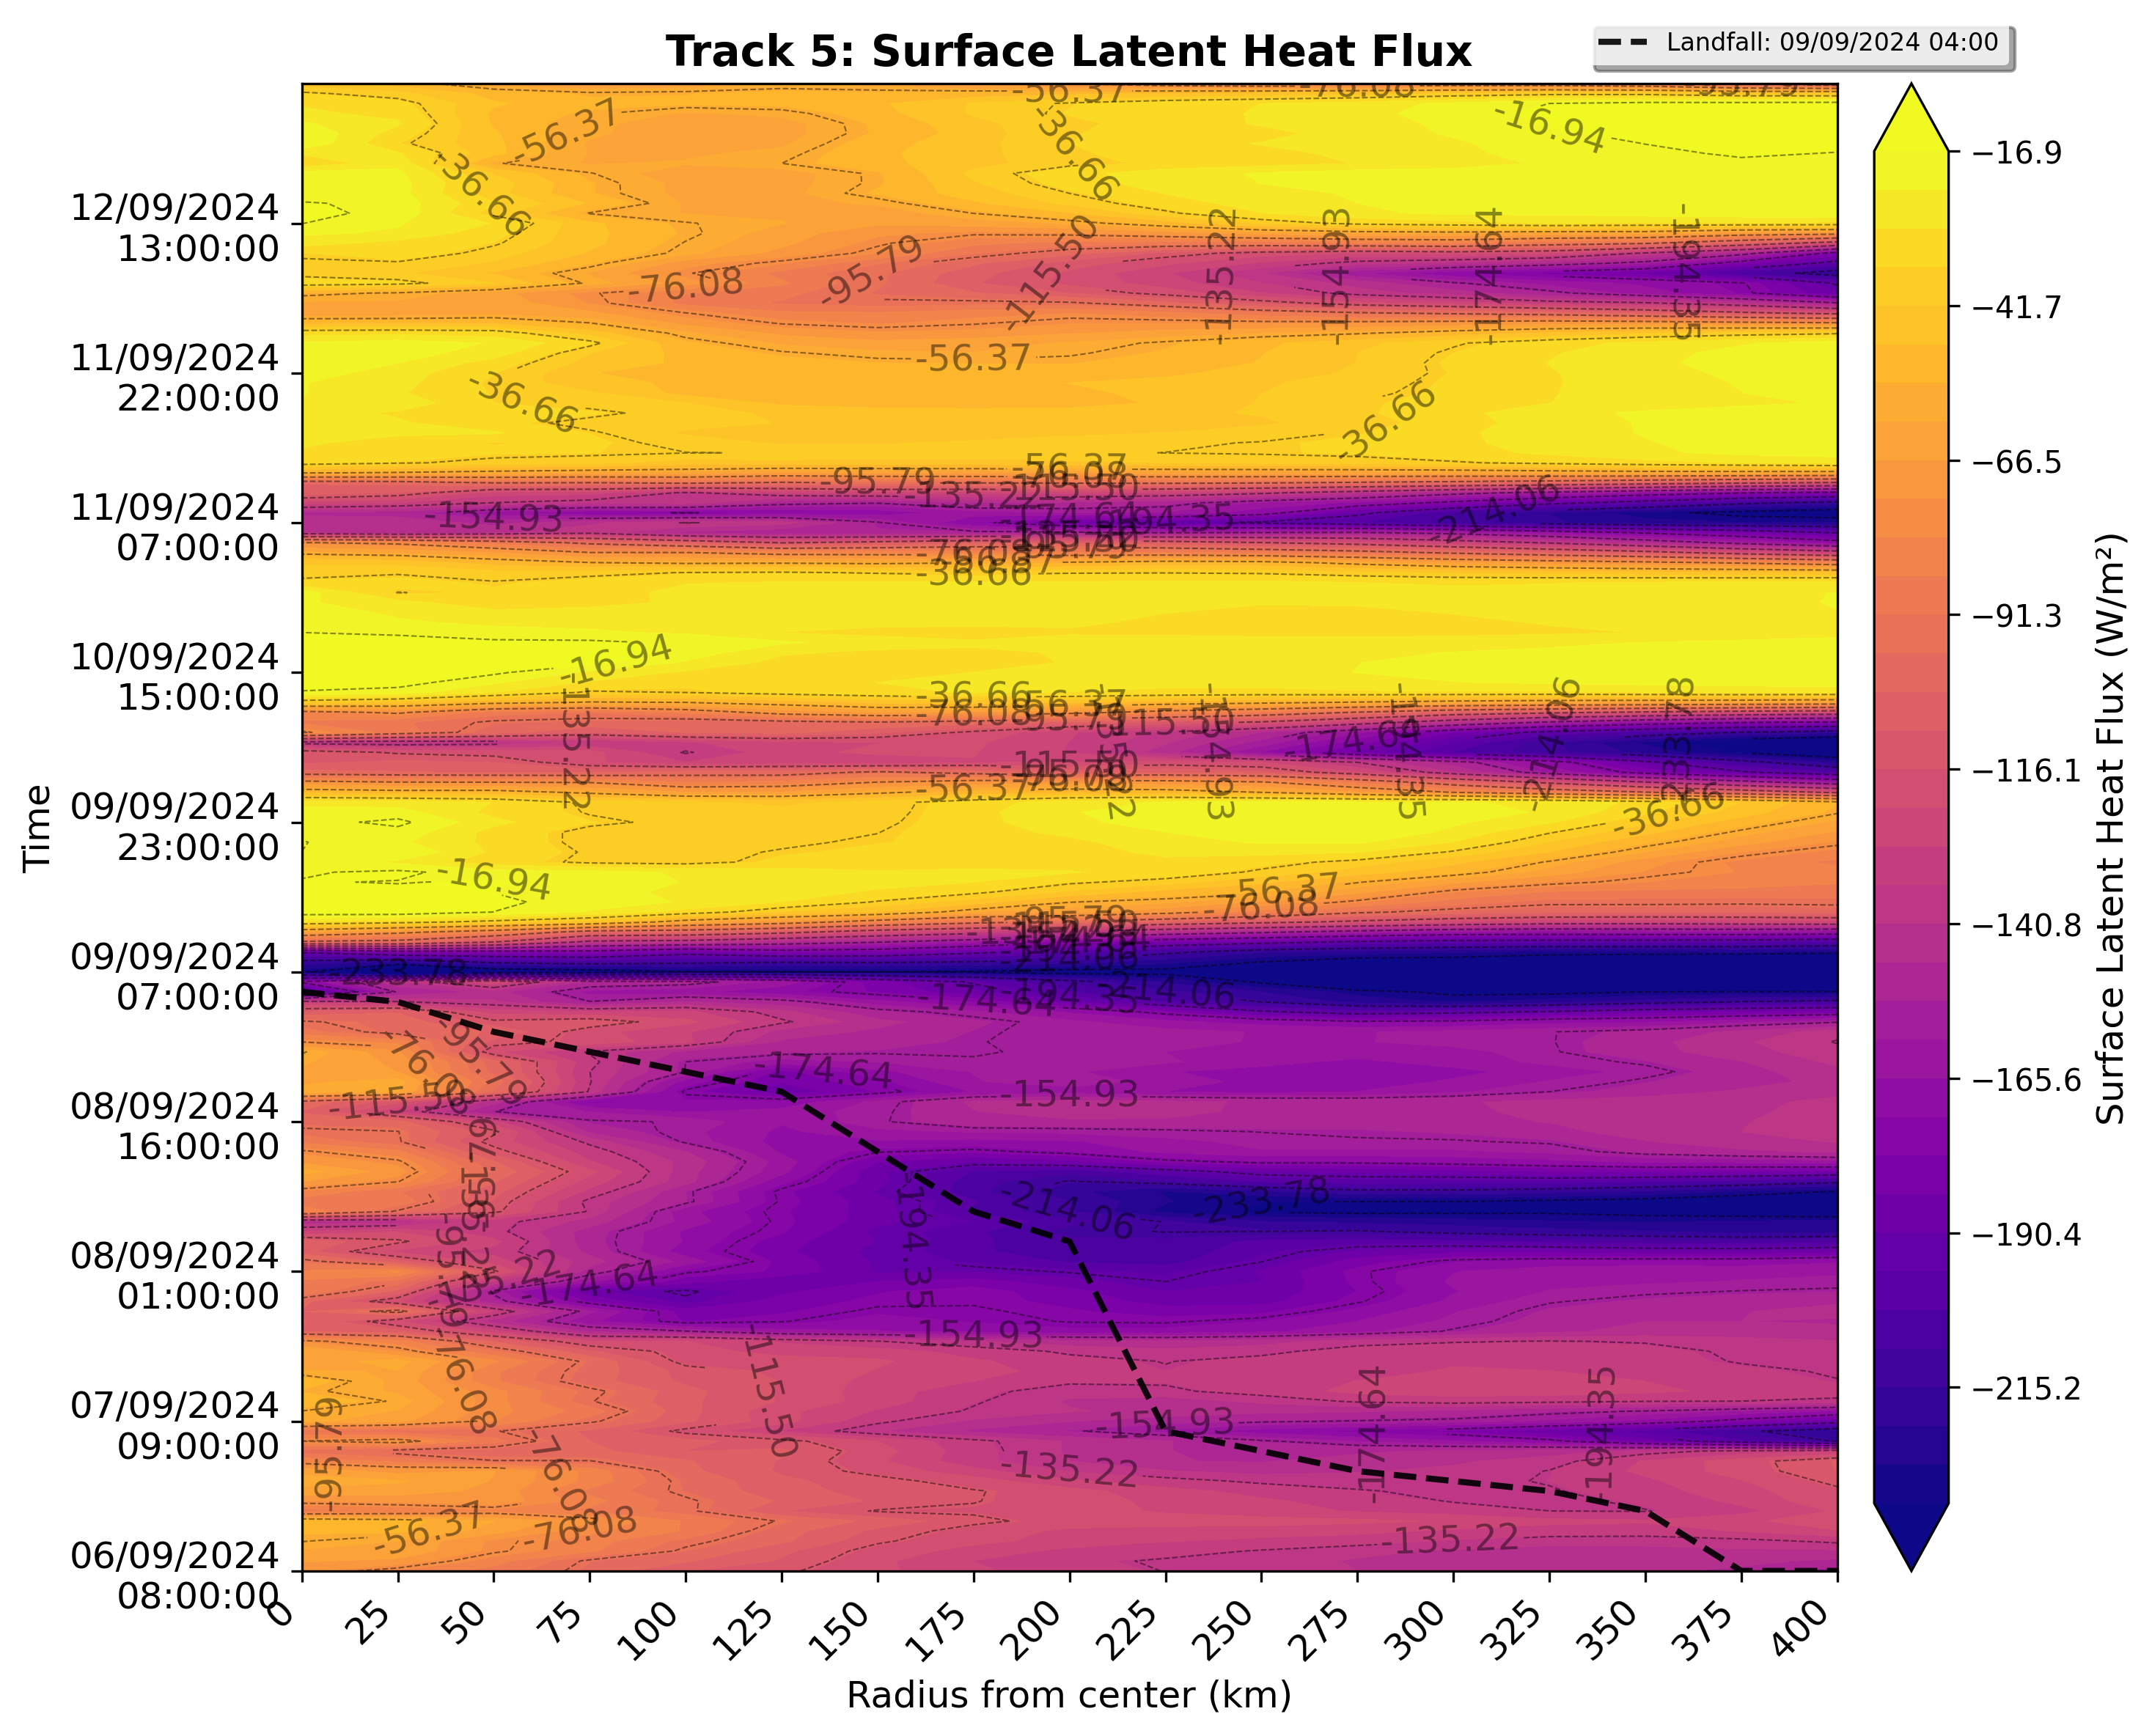
\includegraphics[width=0.91\textwidth]{track_long_slhtf_hov}
      \caption{\scriptsize \textbf{BOE-Active:} Inner-core LHF
        remains above the $70$ W\,m$^{-2}$ sustaining threshold for $>48$ h
      inland, effectively mimicking the oceanic energy conditions.}
    \end{figure}

    \column{0.50\textwidth}
    \vspace{-1.22cm}
    \begin{figure}
      \centering
      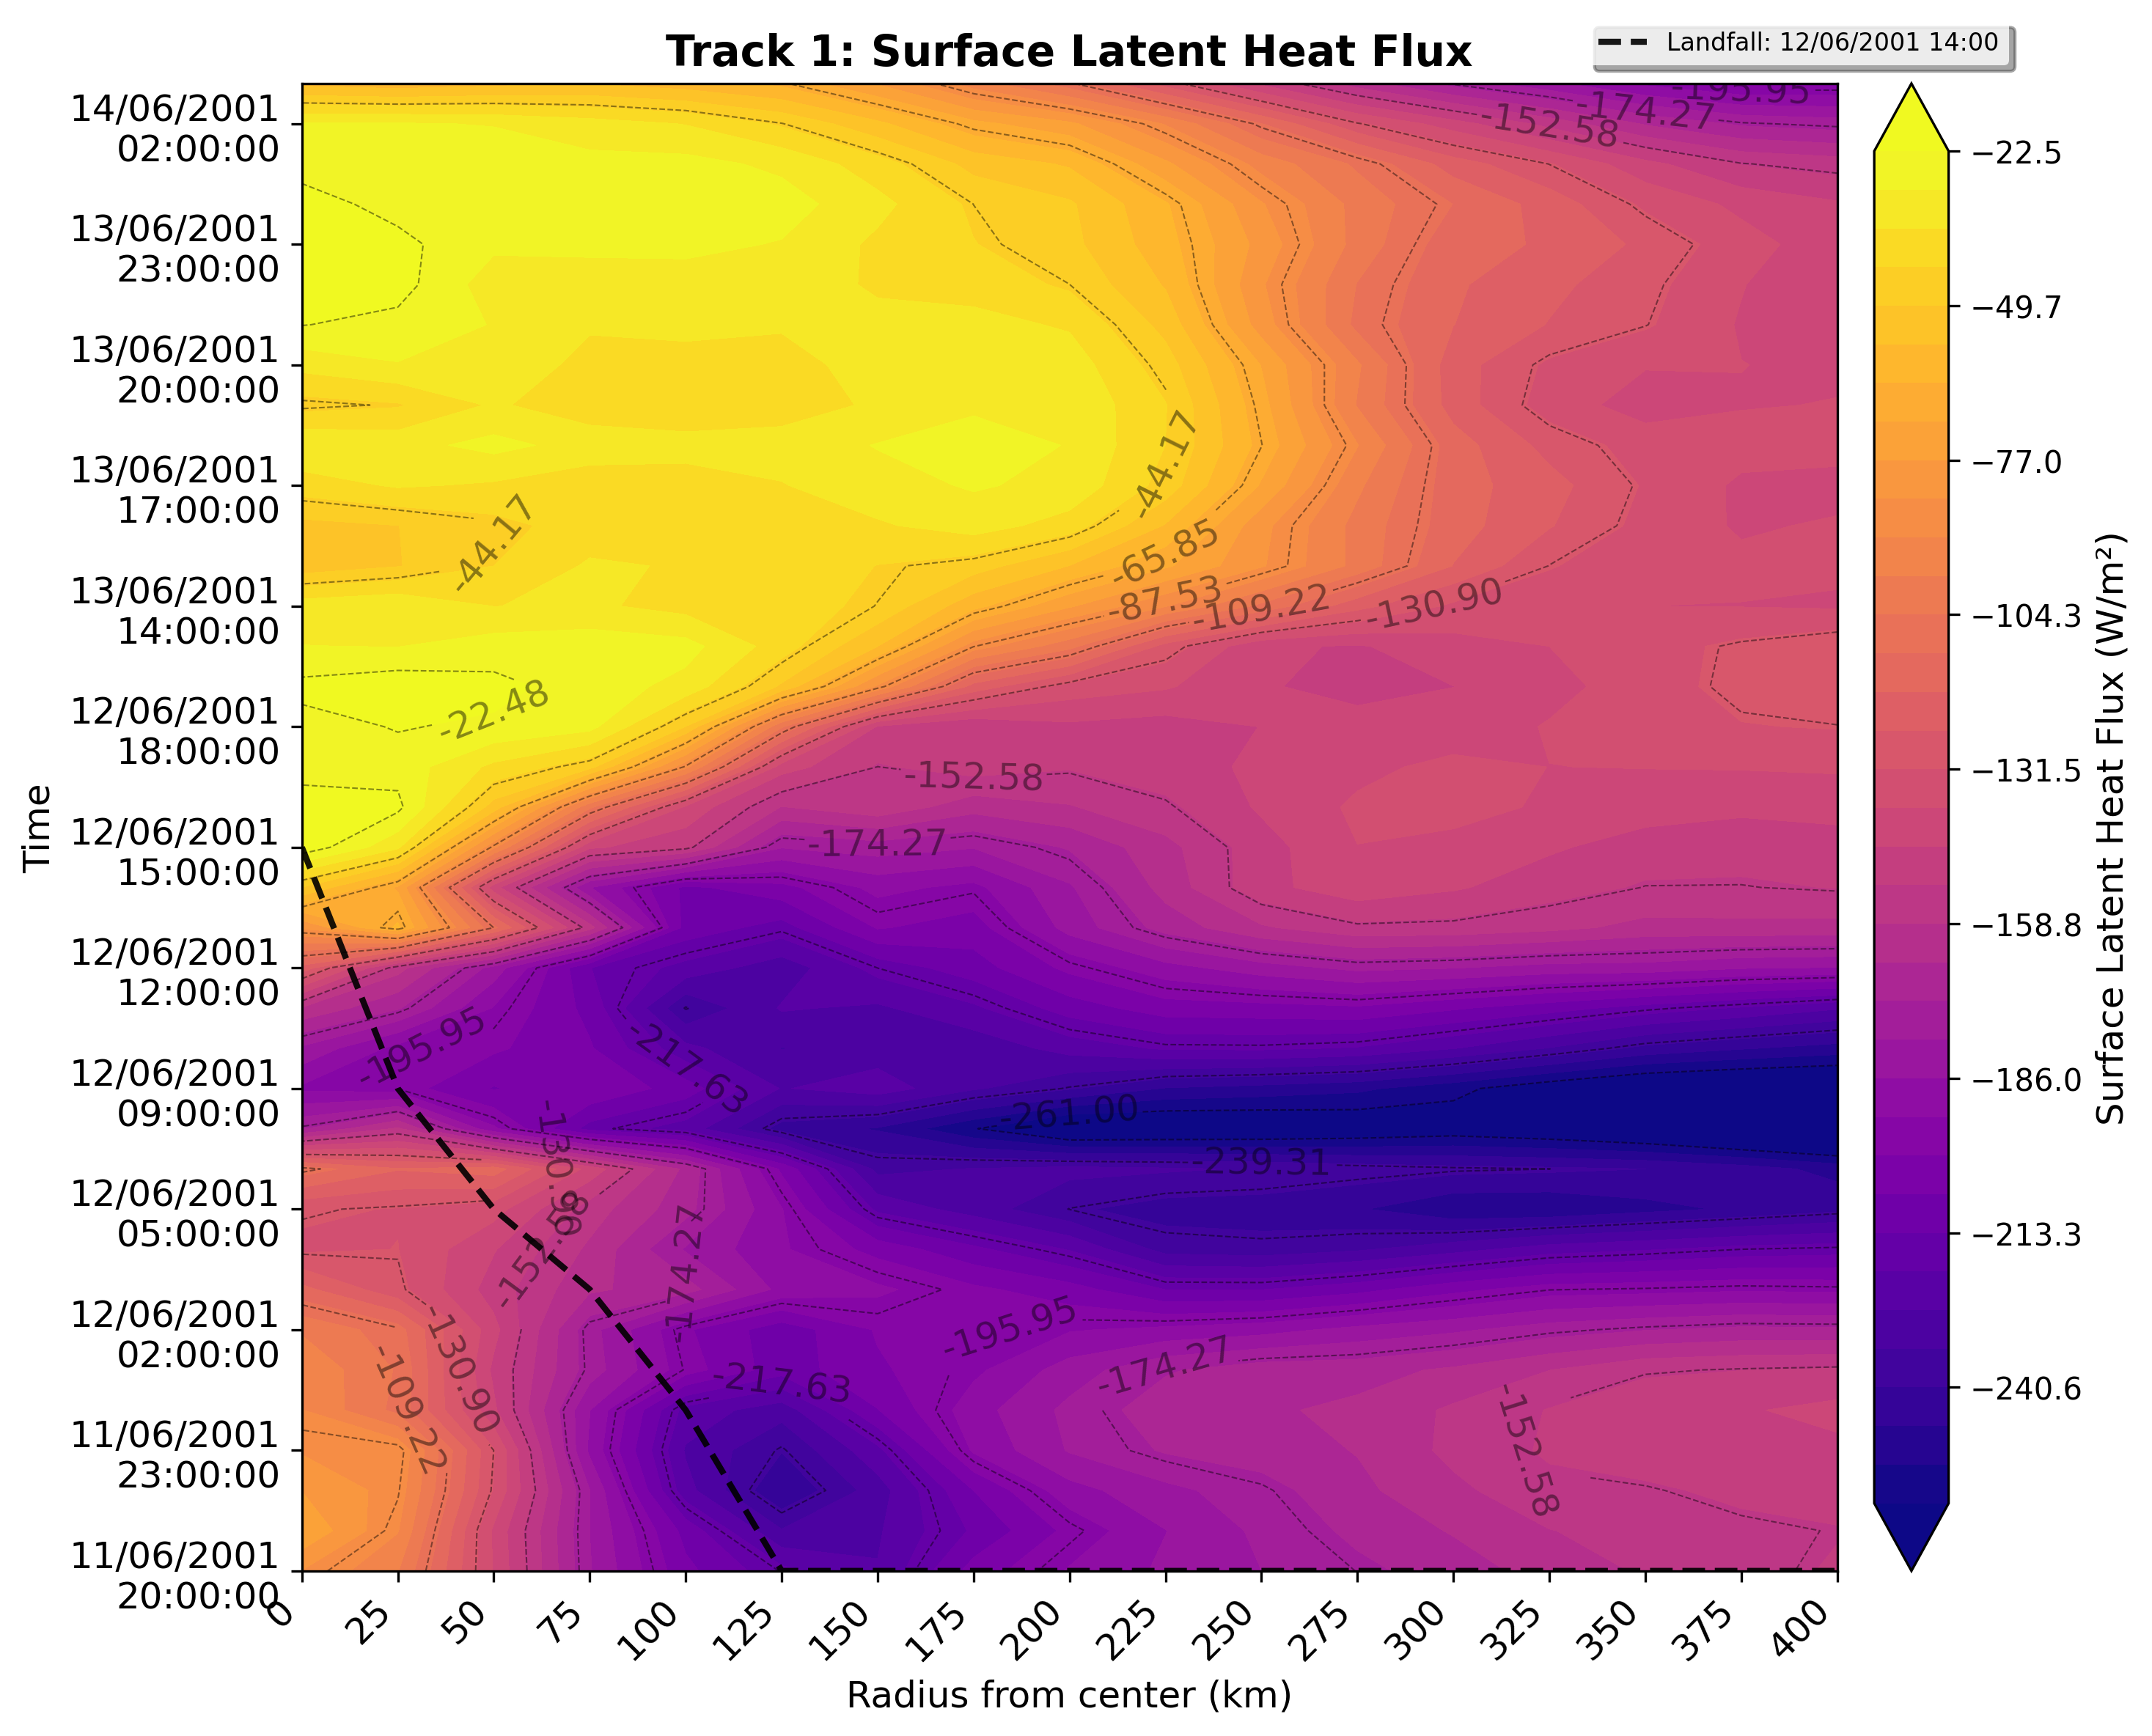
\includegraphics[width=0.91\textwidth]{track_short_slhtf_hov}
      \caption{\scriptsize \textbf{Non-BOE:} Despite similar
        oceanic LHF before landfall (150-220 W m$^{-2}$), flux collapses
      within \textbf{12-18 h} of landfall - insufficient soil reservoir.}
    \end{figure}
  \end{columns}

  \vspace{-0.15cm}
  \scriptsize
  The BOE Energy Crossover: Both systems arrive at the coast with
  well-organized vorticity and high oceanic LHF. The divergence is
  entirely determined by what the land surface provides
  post-landfall. Saturated soil $\Rightarrow$ energy-limited
  evaporation (sustained LHF); dry soil $\Rightarrow$ water-limited
  evaporation (rapid collapse).
\end{frame}

% ---------------------------------------------------------Slide:
% SHF - Thermal Feedback
\setLayout{plain}
\begin{frame}{Sensible Heat Flux: Thermal Stabilization in BOE Systems}
  \begin{columns}
    \column{0.50\textwidth}
    \vspace{-1.21cm}
    \begin{figure}
      \centering
      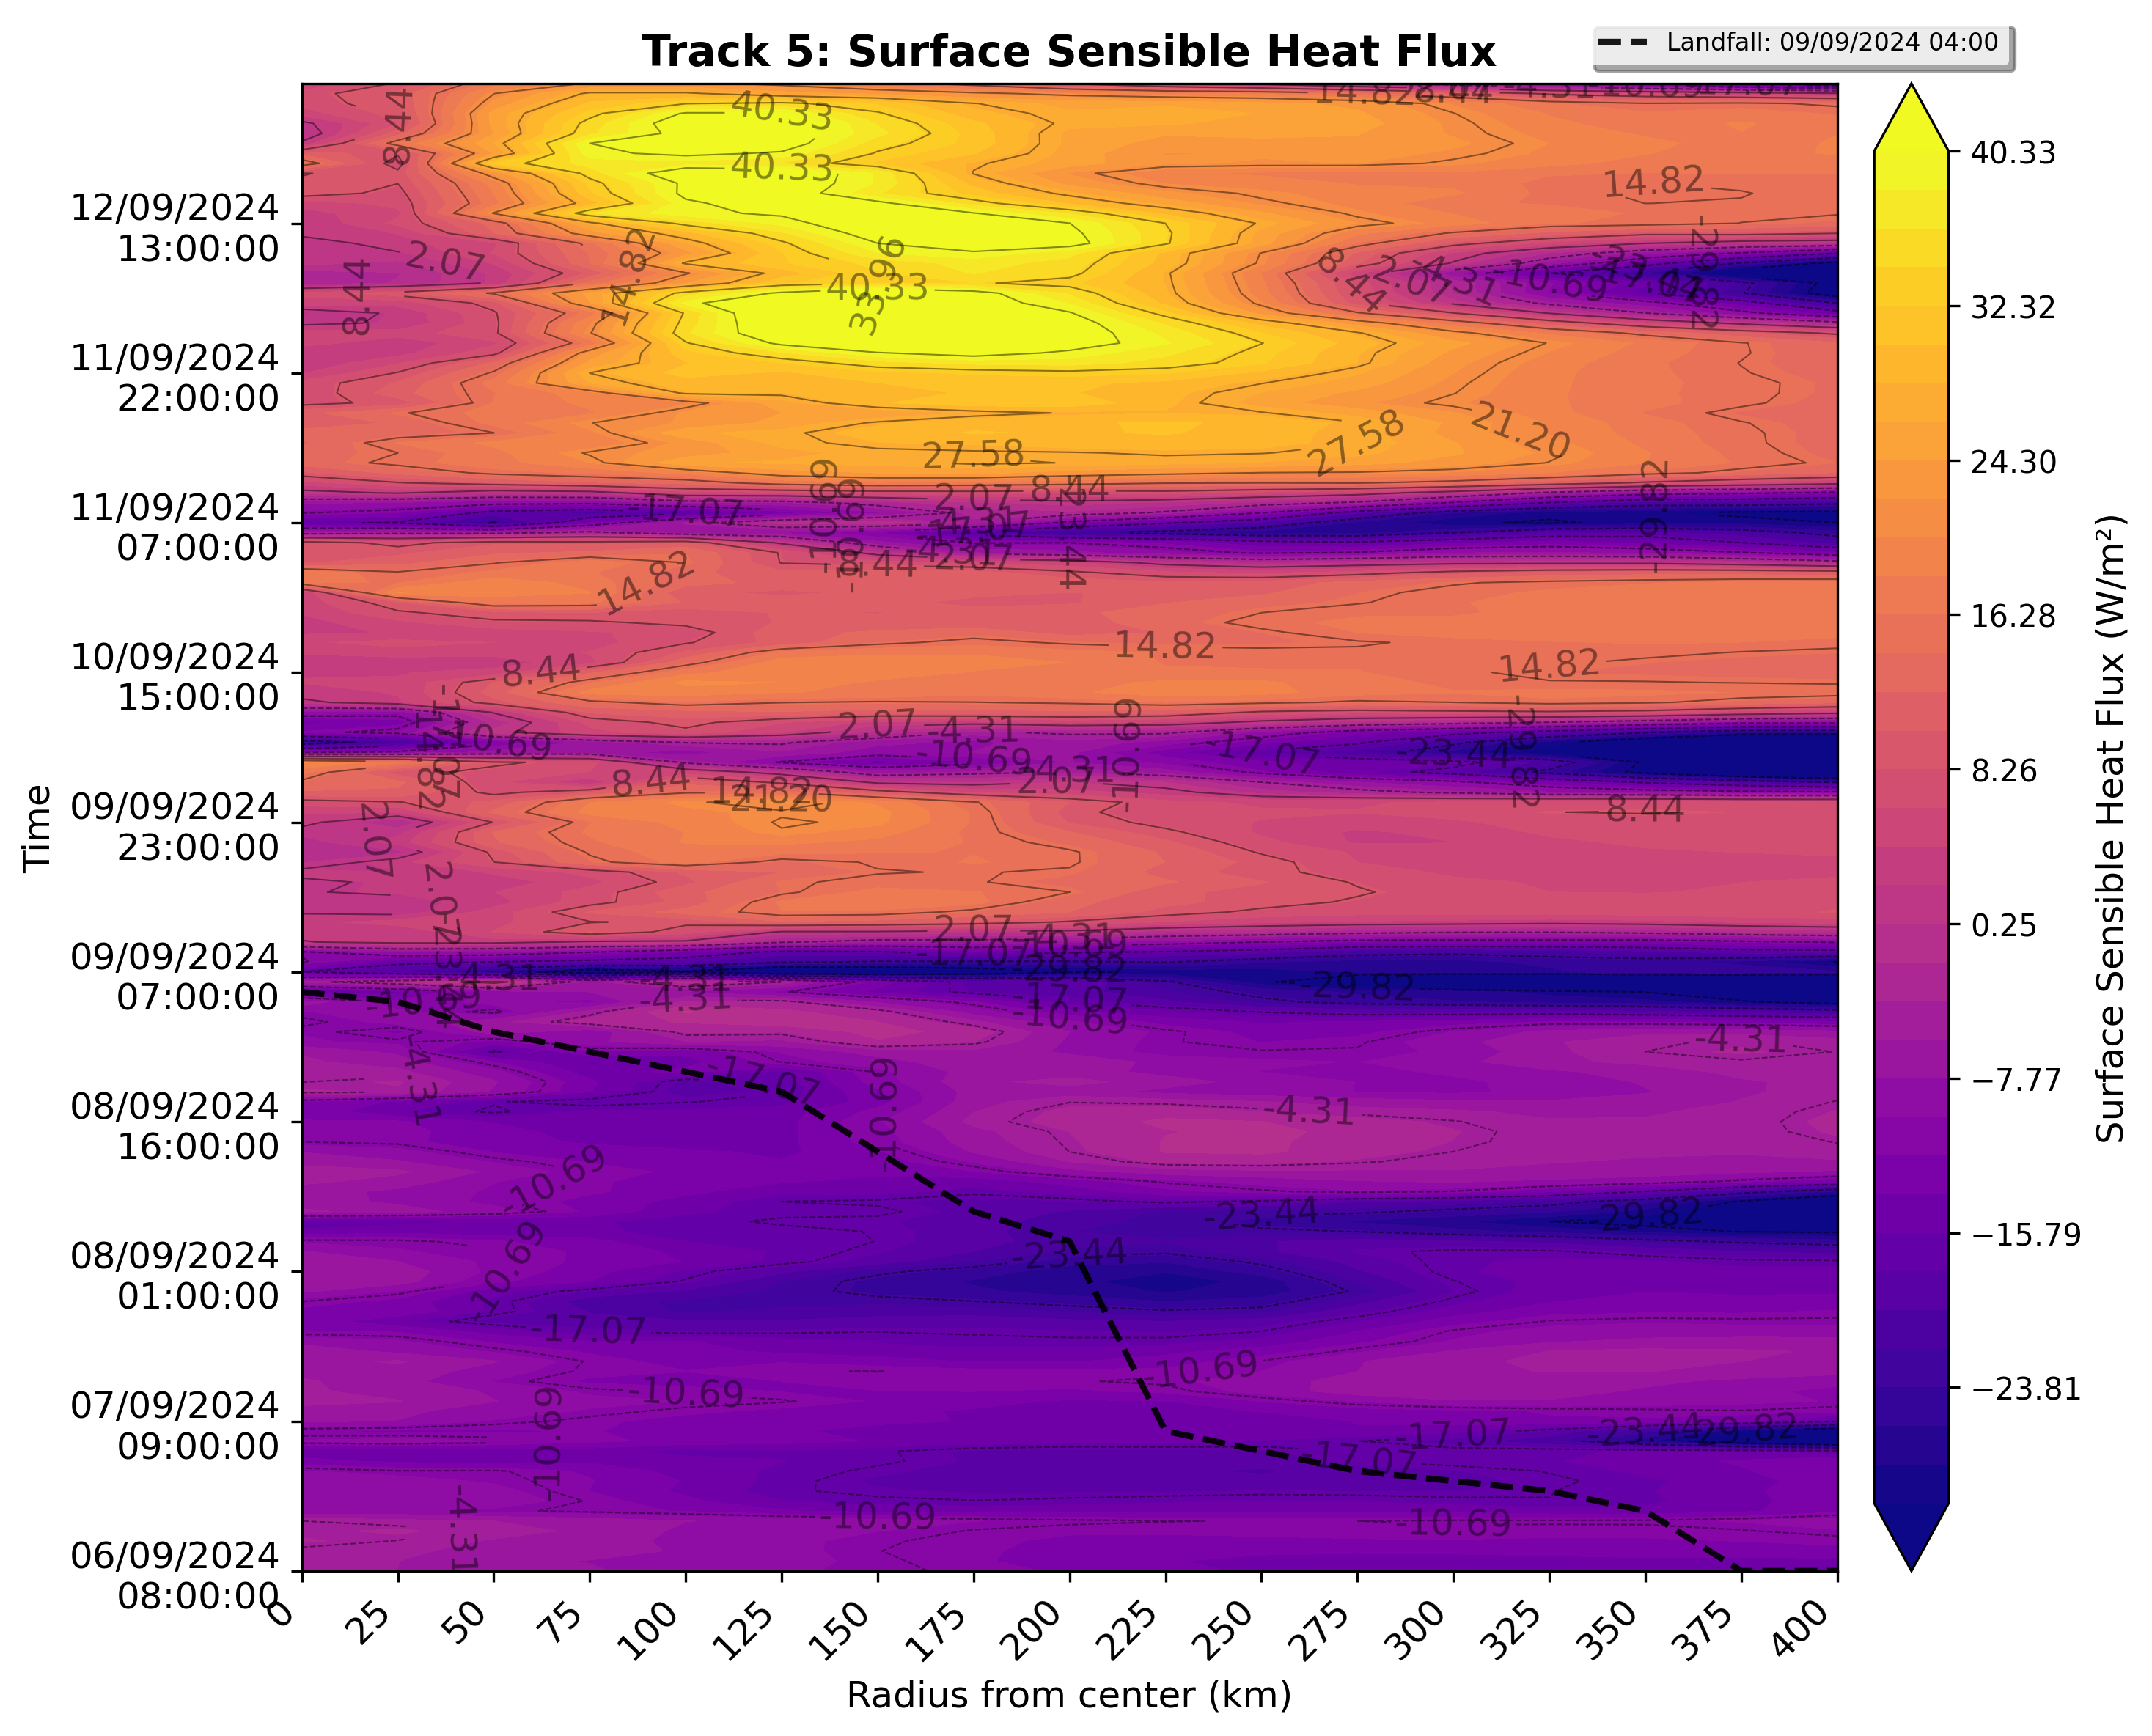
\includegraphics[width=0.91\textwidth]{track_long_ishf_hov}
      \caption{\scriptsize \textbf{BOE-Active:} SHF remains
        suppressed after landfall - energy partitioned into latent heat.
      Cool, moist boundary layer preserved, vortex structurally maintained.}
    \end{figure}

    \column{0.50\textwidth}
    \vspace{-1.21cm}
    \begin{figure}
      \centering
      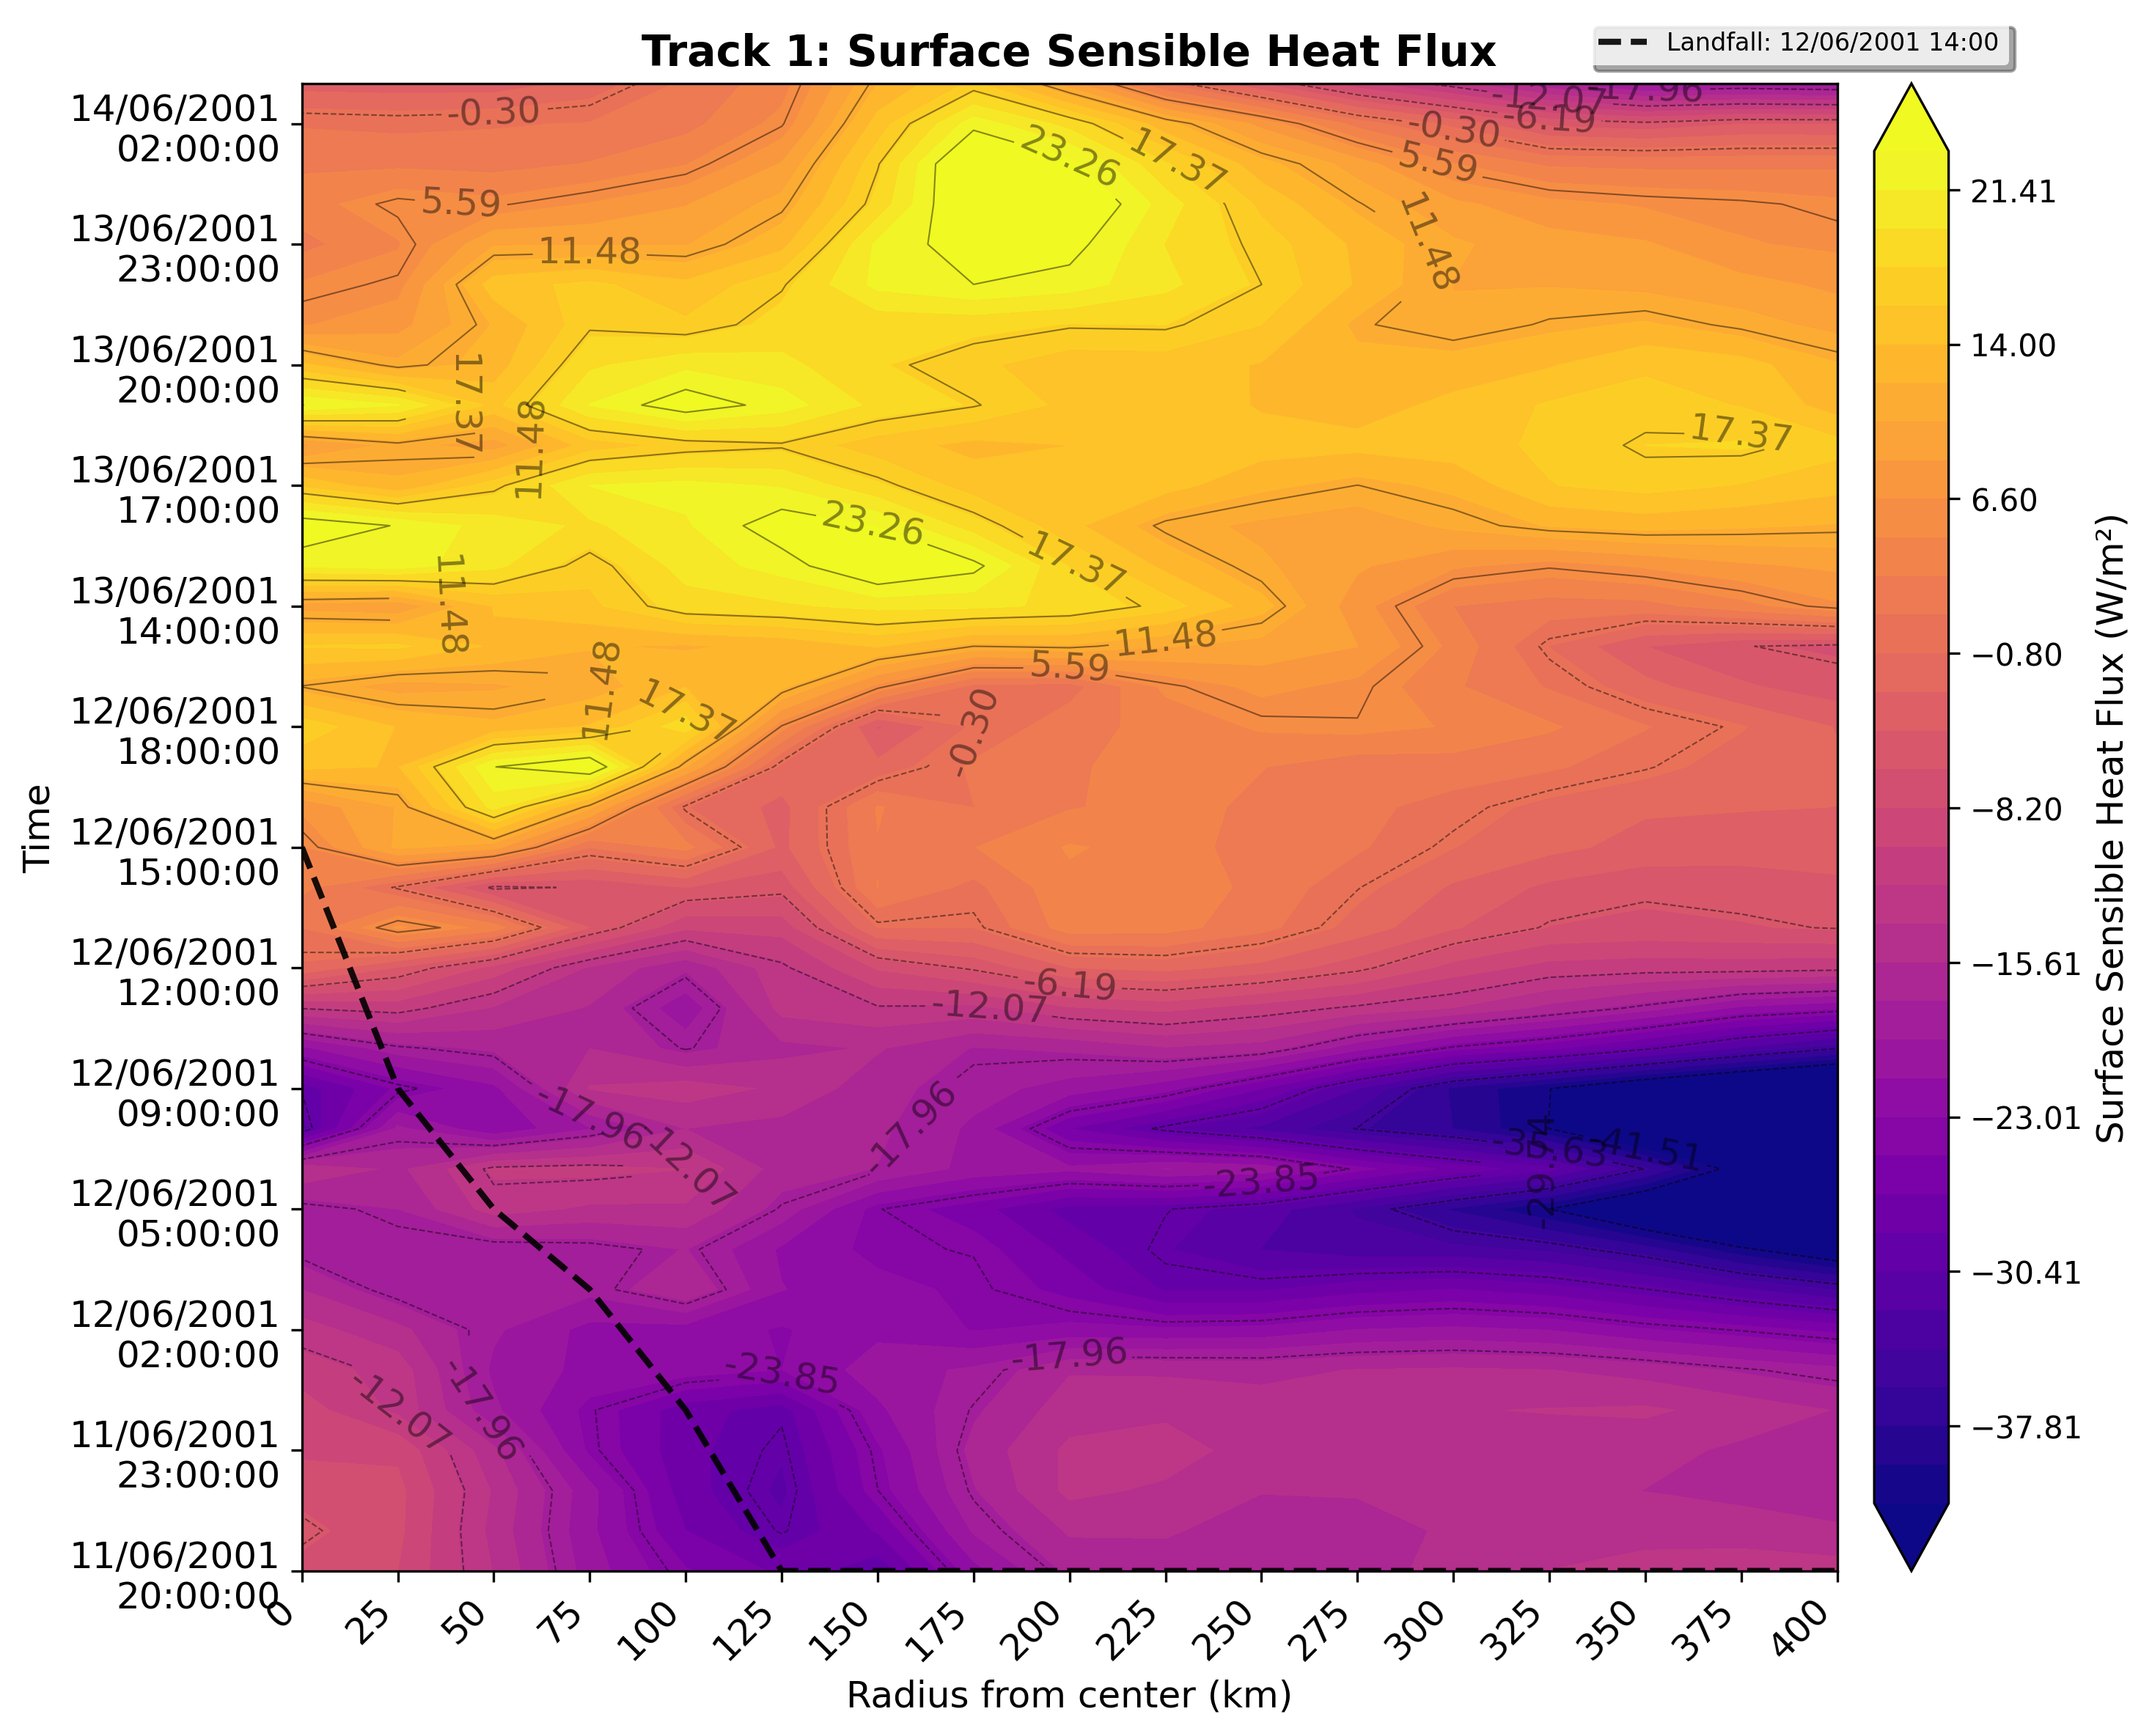
\includegraphics[width=0.91\textwidth]{track_short_ishf_hov}
      \caption{\scriptsize \textbf{Non-BOE:} Extreme SHF
        fluctuations at landfall (21 to $-37$ W\,m$^{-2}$) - hot, dry
        surface heats BL, raises LCL, encourages dry-air entrainment
      $\Rightarrow$ rapid structural collapse.}
    \end{figure}
  \end{columns}

  \vspace{-0.15cm}
  \scriptsize
  Bowen Ratio Interpretation : BOE-active systems maintain $\beta
  \approx 0.1$-$0.3$ (ocean-like) post-landfall. Non-BOE systems
  transition to $\beta > 1$ (dry land regime) within hours, marking
  the shift from energy-limited to water-limited evaporation.
\end{frame}

%---------------------------------------------------------Slide: Dew Point
\setLayout{plain}
\begin{frame}{Dew Point Temperature: Boundary Layer Saturation}
  \begin{columns}
    \column{0.50\textwidth}
    \vspace{-1.22cm}
    \begin{figure}
      \centering
      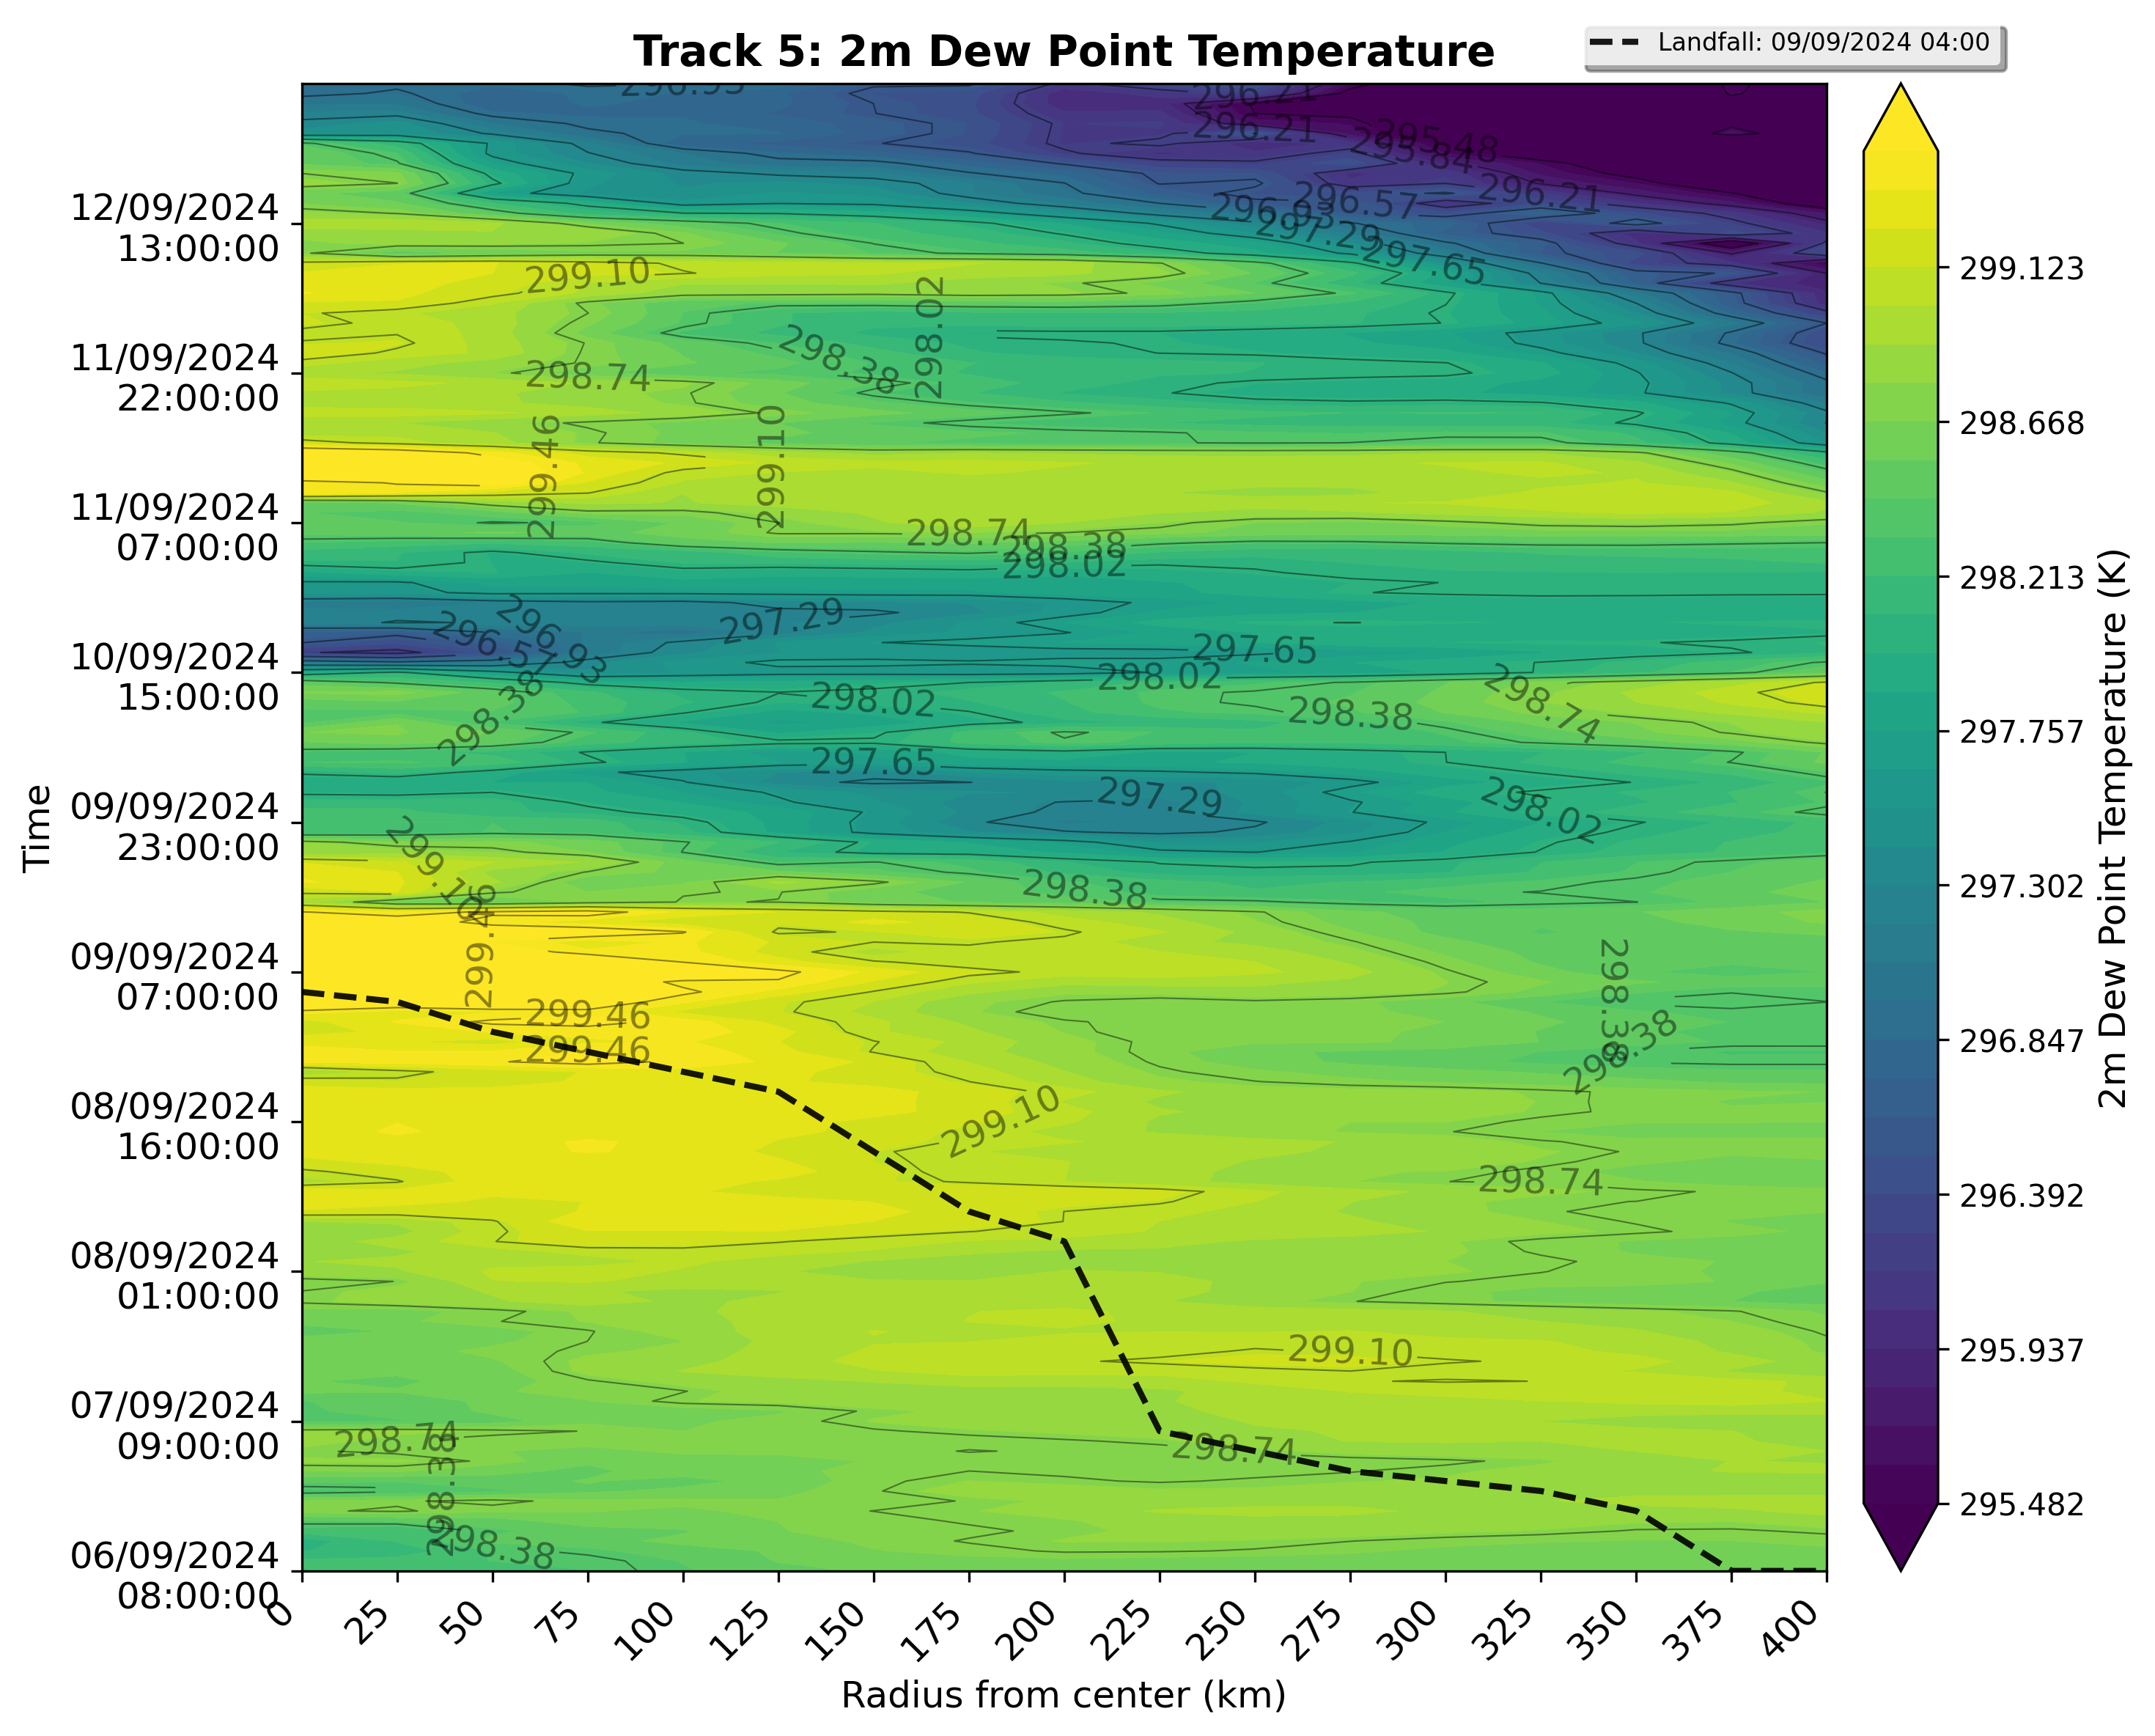
\includegraphics[width=0.90\textwidth]{track_long_d2m_hov}
      \caption{\scriptsize \textbf{BOE-Active:} D2M maintained
        above 298 K for $>72$ h - near-saturated maritime boundary layer
      preserved deep inland. Dew Point Depression (DPD) $<3$ K throughout.}
    \end{figure}

    \column{0.50\textwidth}
    \vspace{-1.22cm}
    \begin{figure}
      \centering
      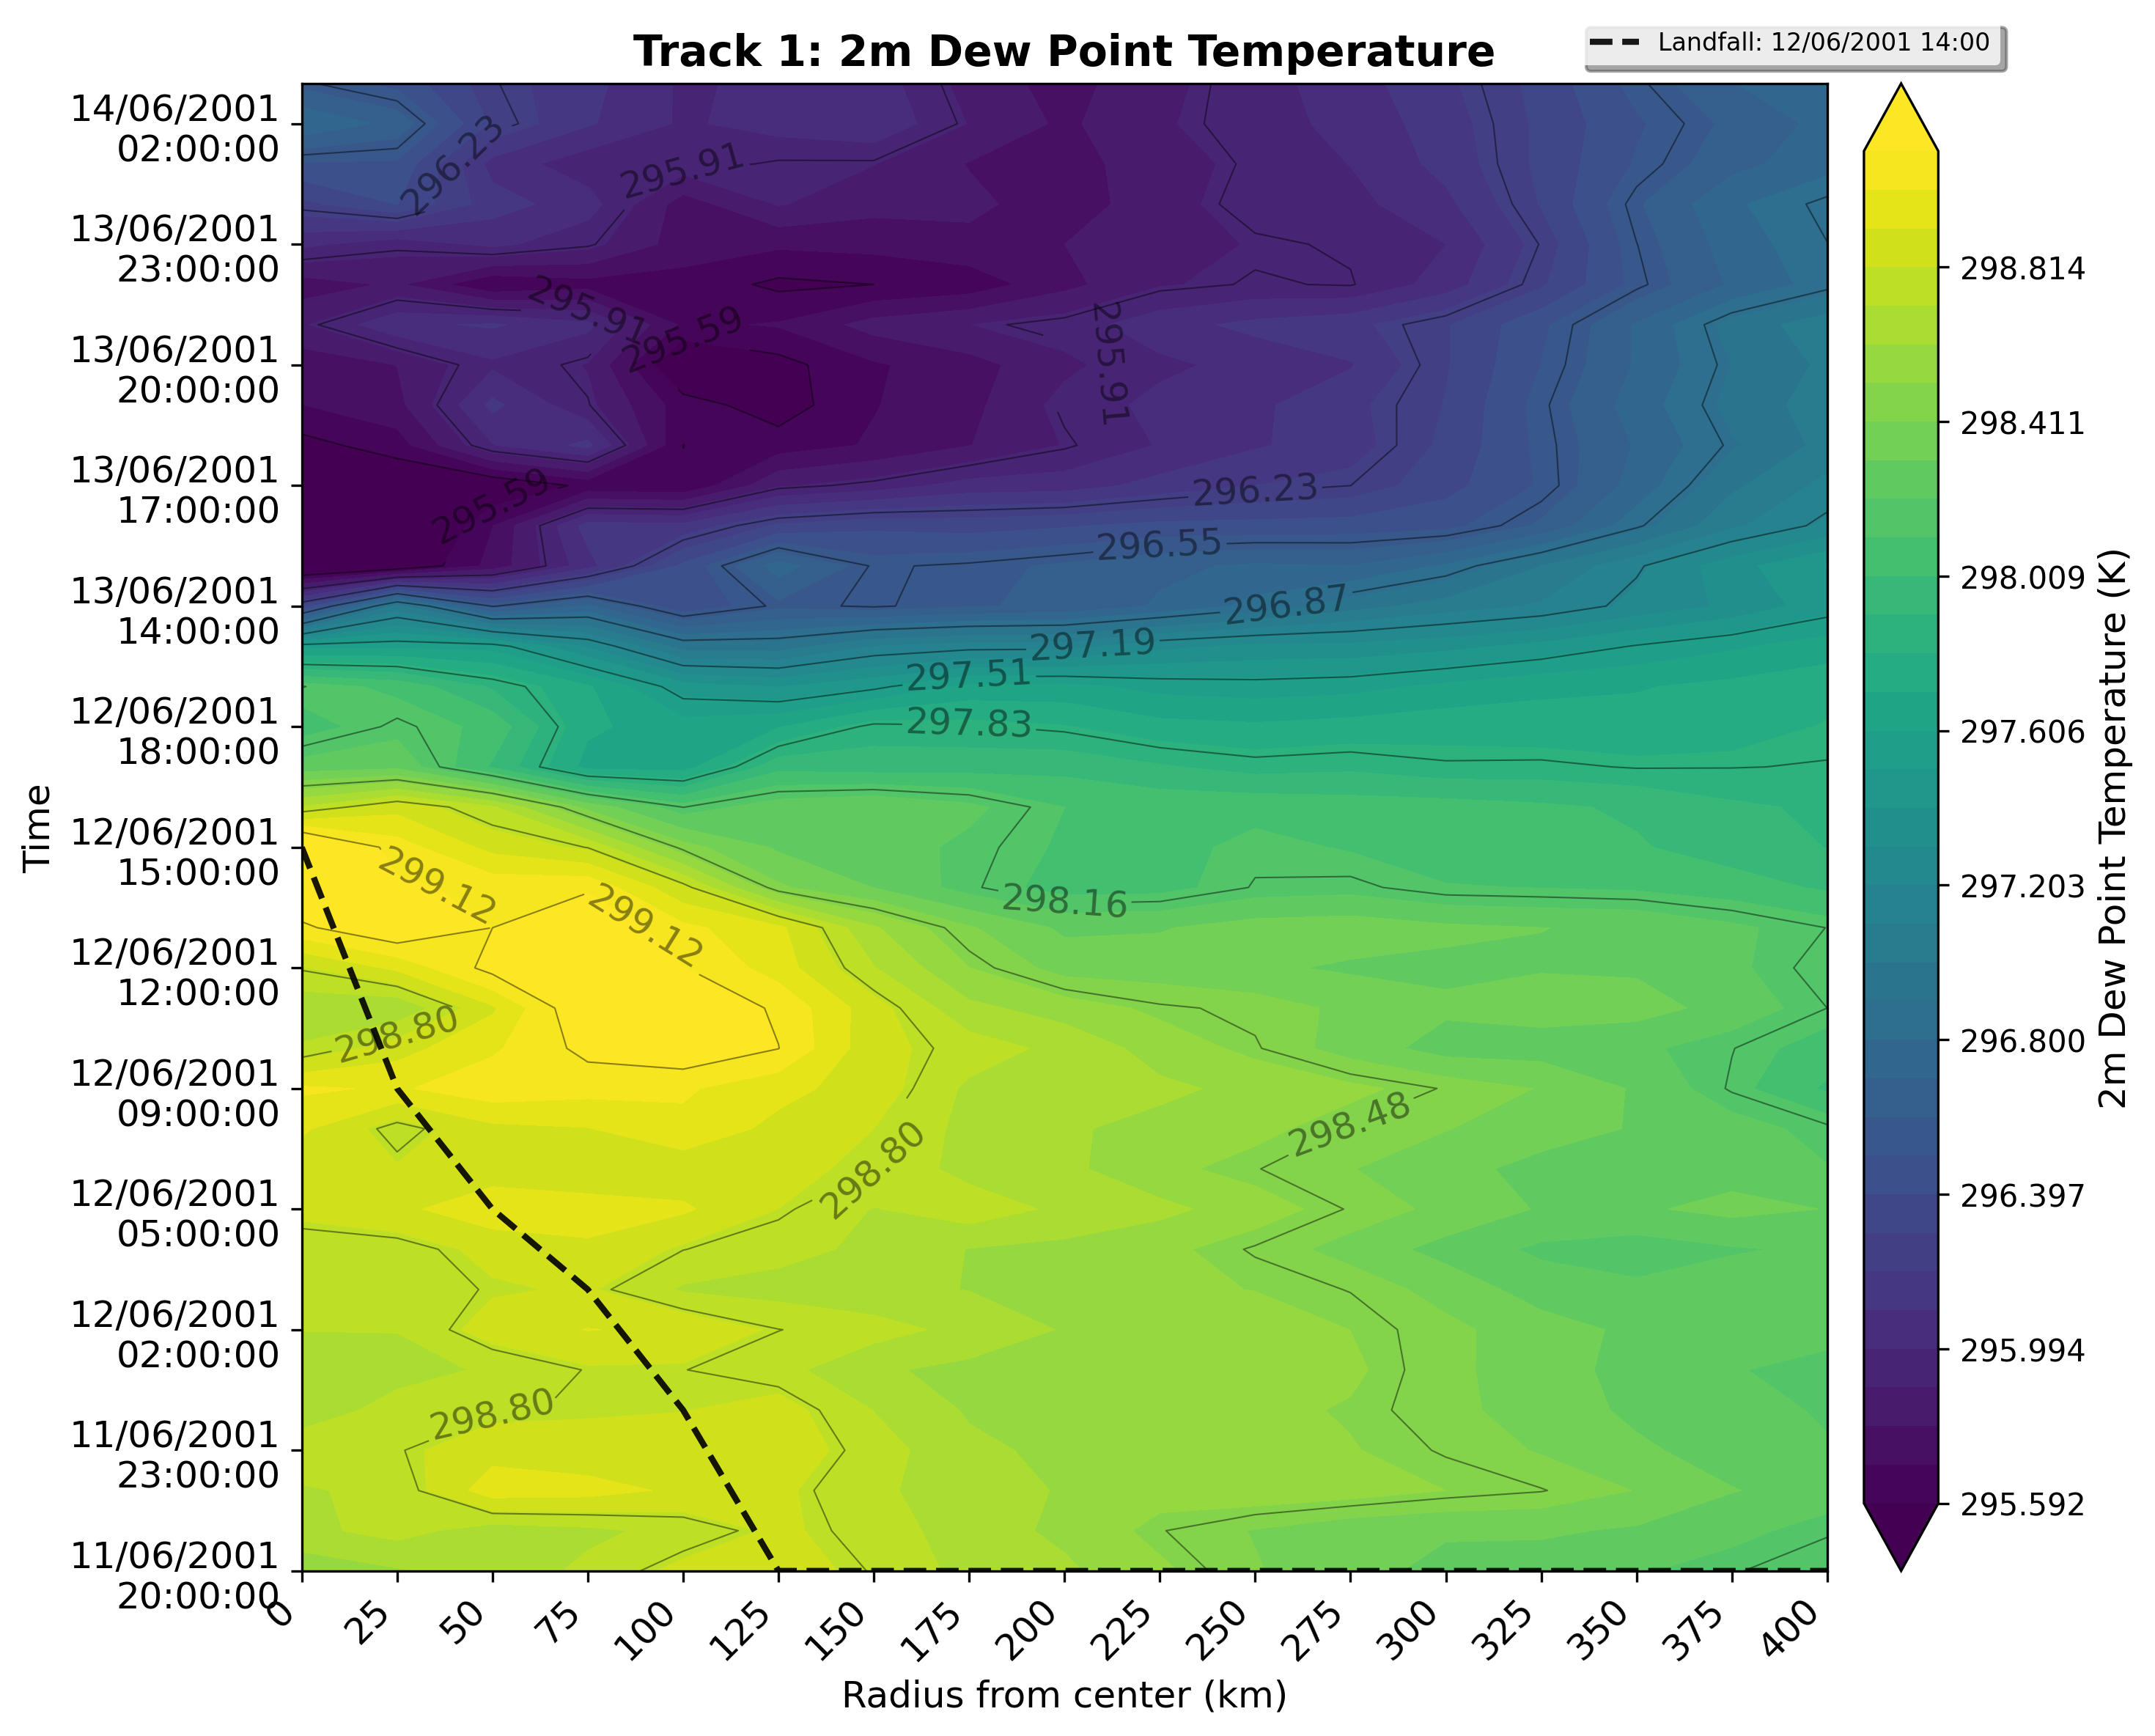
\includegraphics[width=0.90\textwidth]{track_short_d2m_hov}
      \caption{\scriptsize \textbf{Non-BOE:} D2M drops toward 296
        K within 12-24 h. Increased DPD raises the Lifting Condensation
      Level, dissipating core convection.}
    \end{figure}
  \end{columns}

  \vspace{-0.15cm}
  \scriptsize
  The transition from 299 K to 296 K (ocean-like $\rightarrow$
  continental boundary layer) is the thermodynamic dissipation of the
  MD core. BOE-active systems delay this transition indefinitely through
  local moisture recycling - the system carries its own moist
  environment inland.
\end{frame}

\setLayout{mainpoint}
\begin{frame}{}
  \frametitle{RESULTS: EASTERN GHATS INTERACTION}
\end{frame}

%---------------------------------------------------------Slide:
% Elevation Barrier vs. Thermodynamic Escape
\setLayout{plain}
\begin{frame}{Eastern Ghats: Thermodynamic MD Filter, Not An Absolute Barrier}
  \begin{columns}
    \column{0.50\textwidth}
    \vspace{-1.21cm}
    \begin{figure}
      \centering
      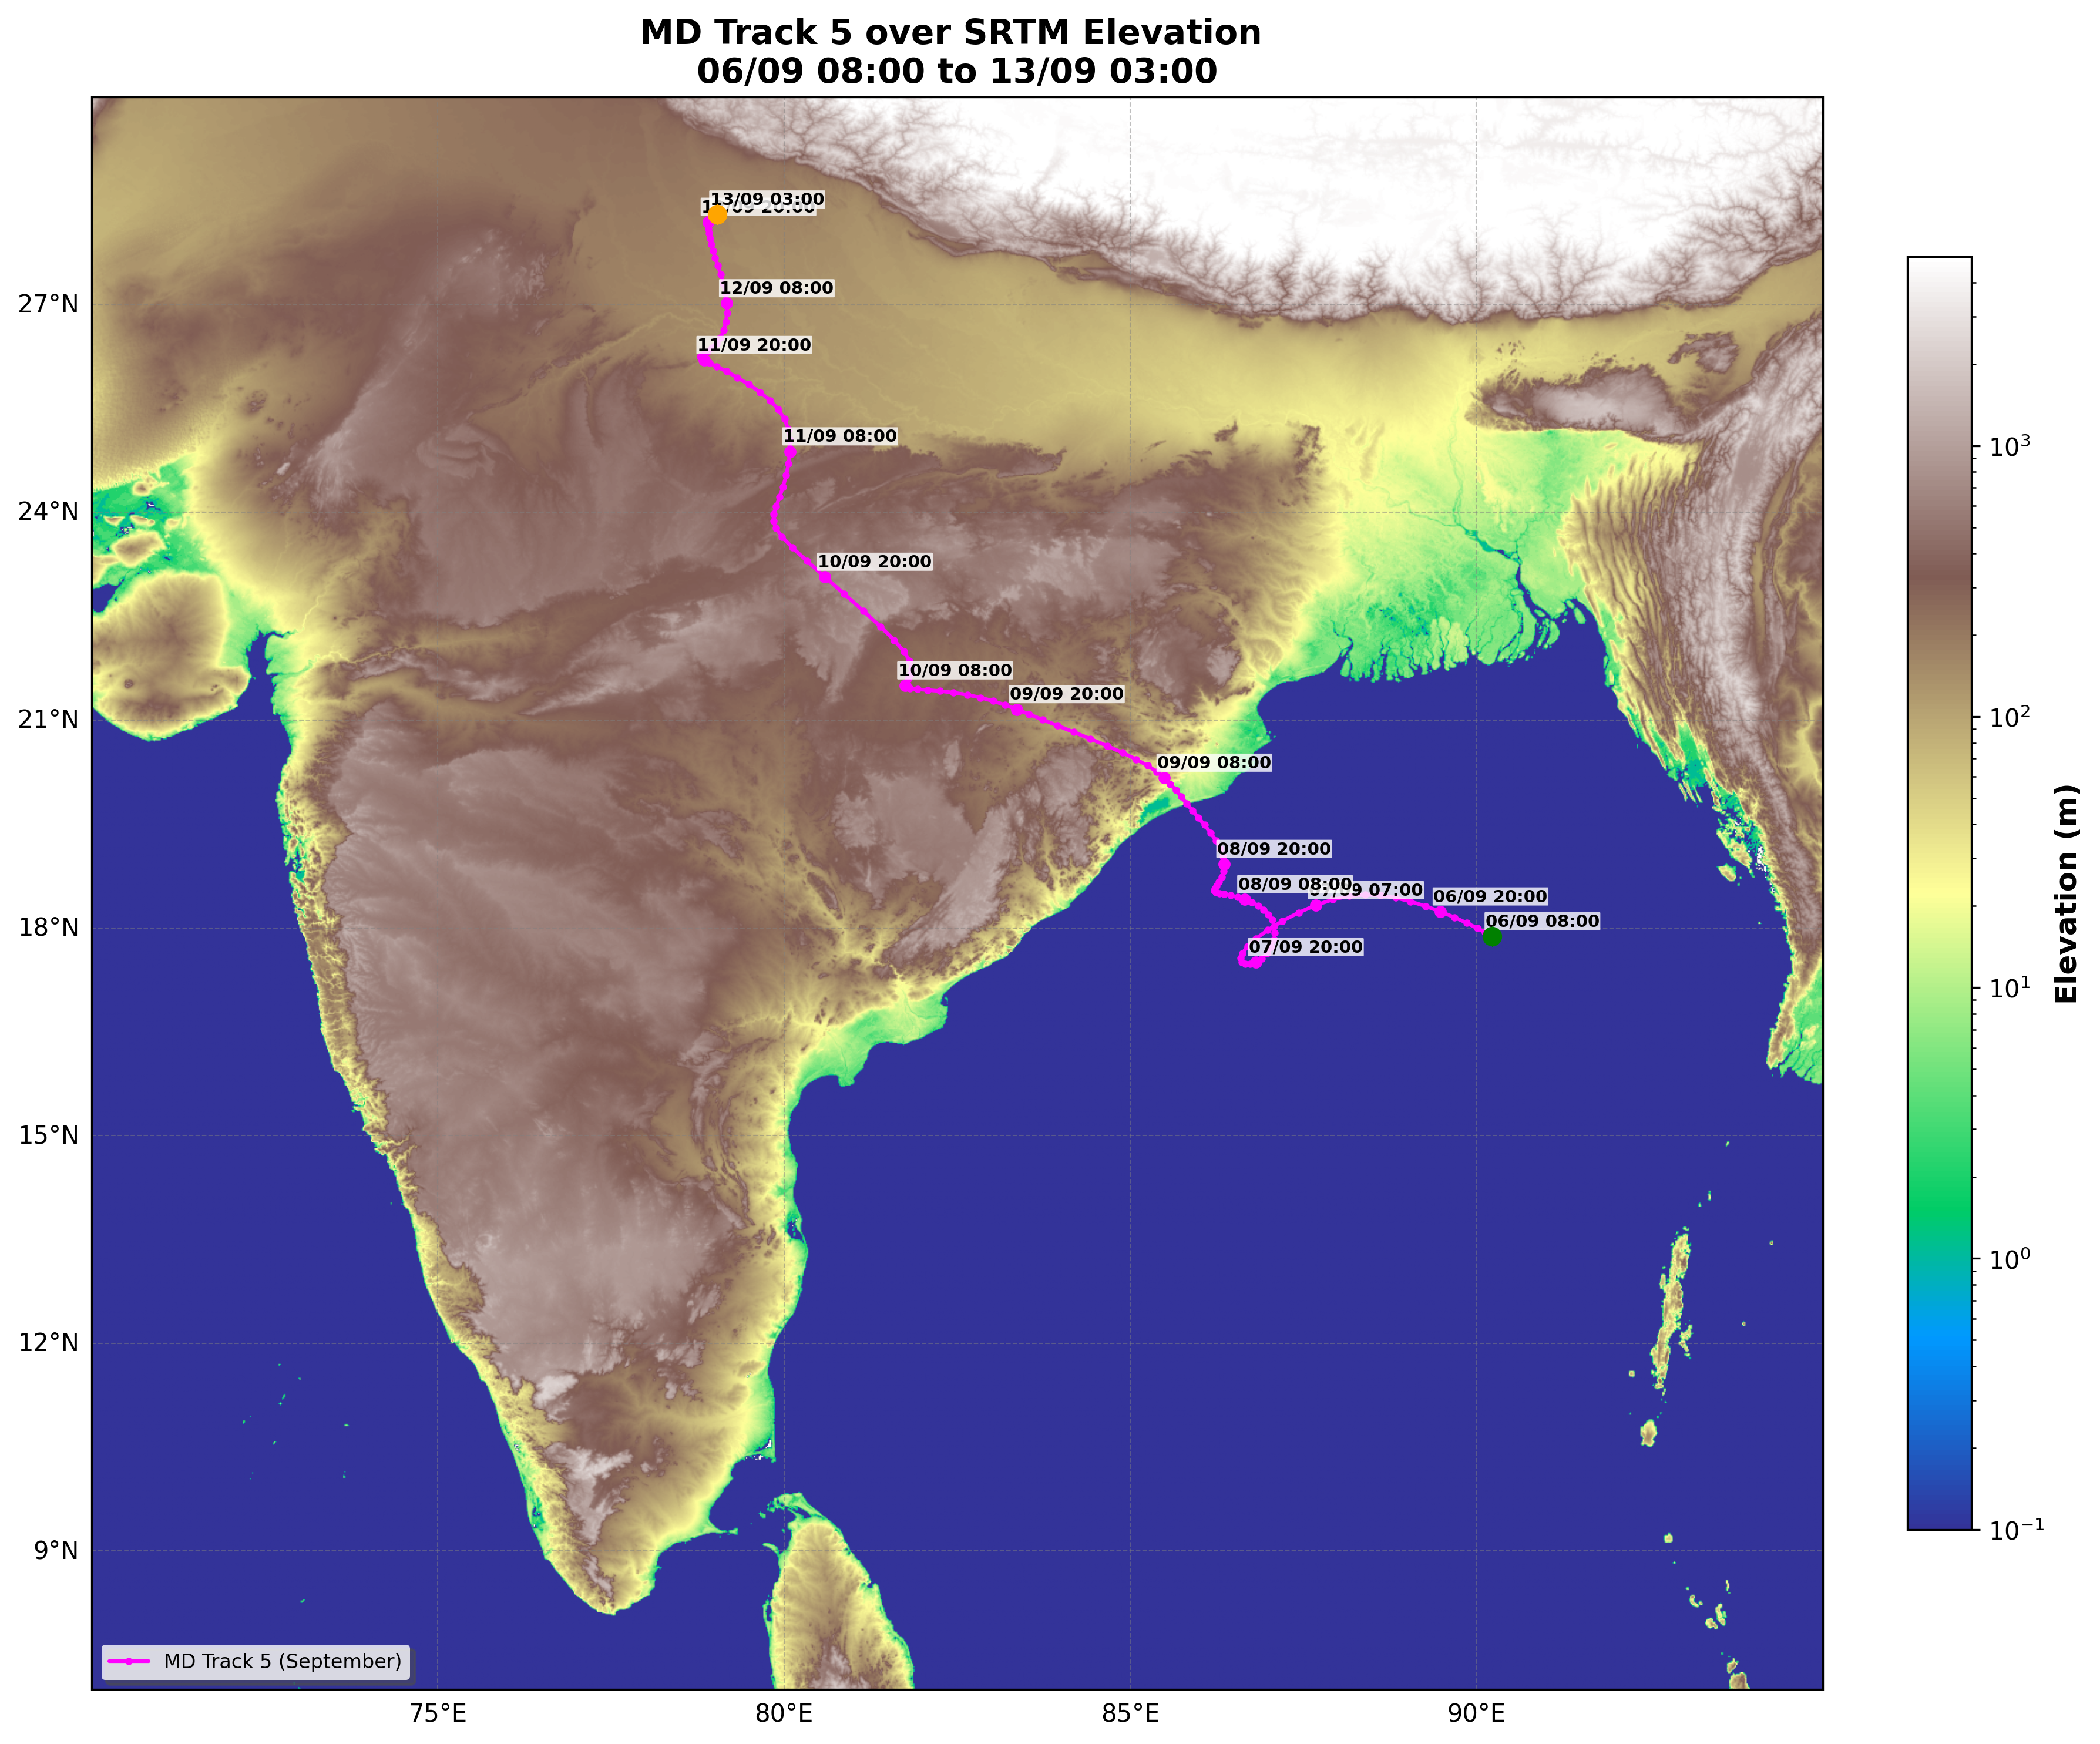
\includegraphics[width=0.87\textwidth]{track_long_elevation_mosaic}
      \caption{\scriptsize \textbf{BOE-Active:} Maintains
        structural integrity across high-relief terrain. Orographic
      precipitation triggers the self-wetting loop; leeward side re-energised.}
    \end{figure}

    \column{0.50\textwidth}
    \vspace{-1.21cm}
    \begin{figure}
      \centering
      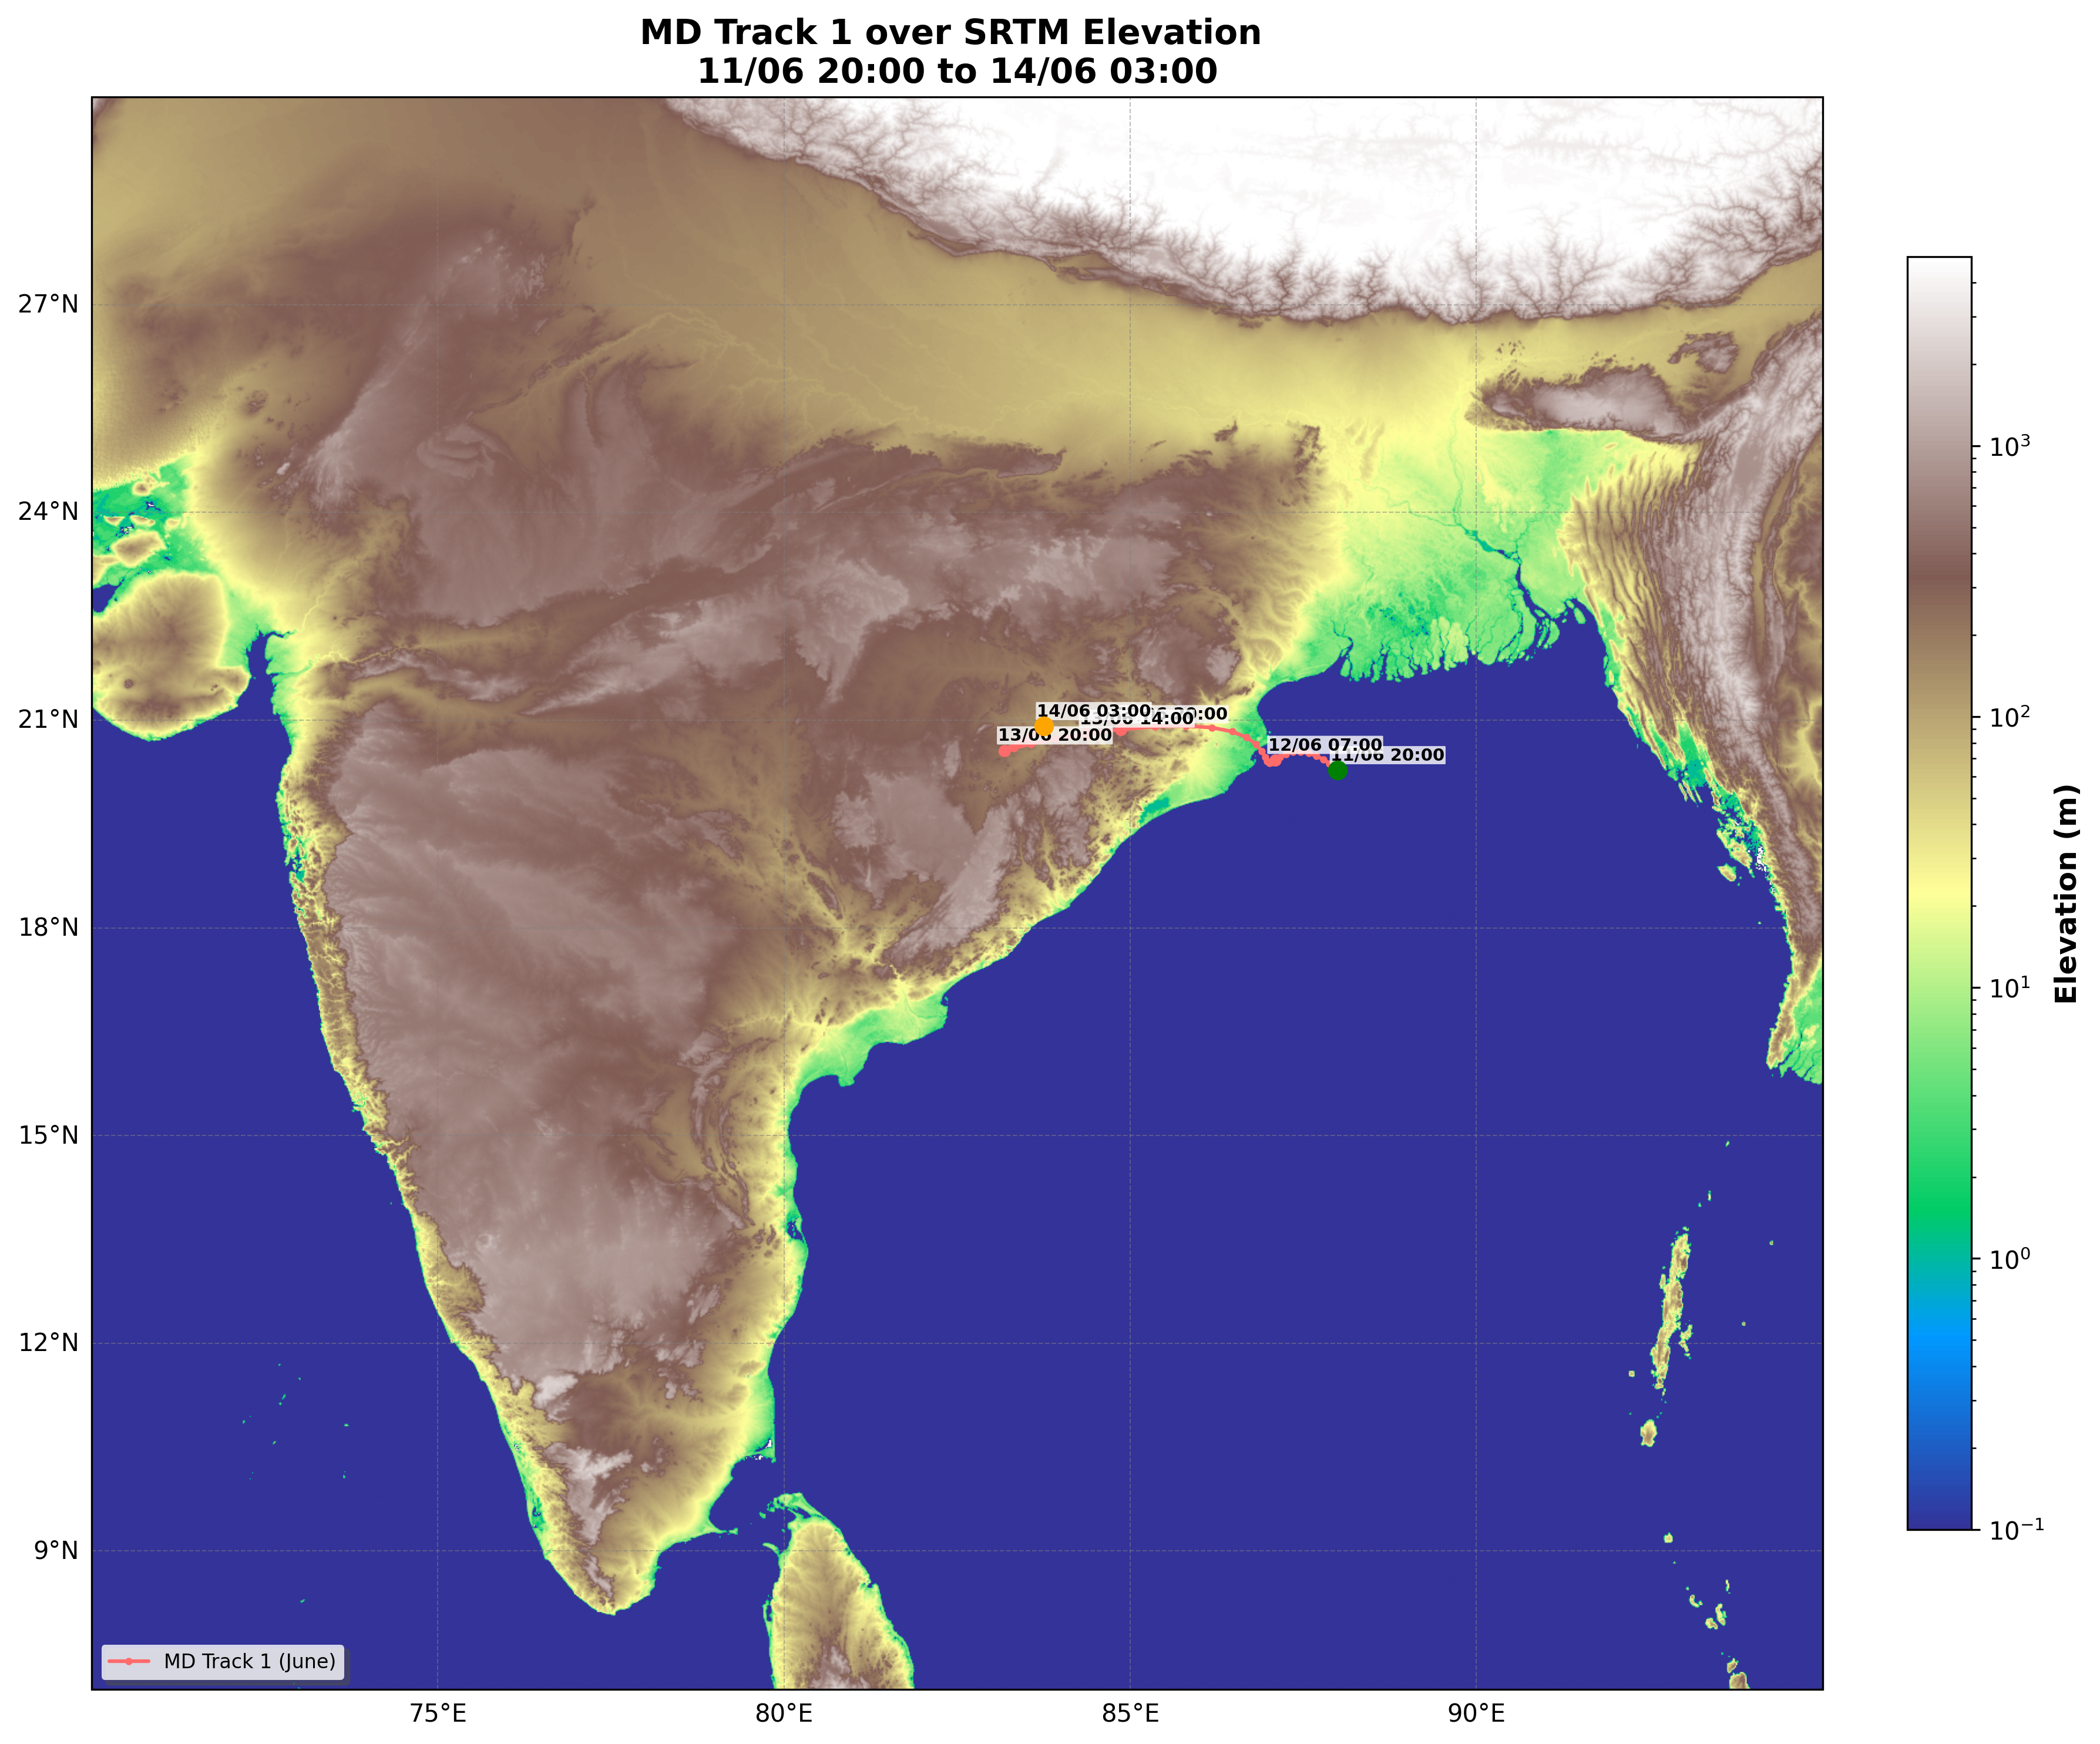
\includegraphics[width=0.87\textwidth]{track_short_elevation_mosaic}
      \caption{\scriptsize \textbf{Non-BOE:} Track terminates
        near the 500 m contour. Orographic moisture stripping due to
        heavy precipitation on windward slopes removes remaining
      energy; no recovery.}
    \end{figure}
  \end{columns}

  \vspace{-0.15cm}
  \scriptsize
  Thermodynamic Escape Mechanism : Both systems experience initial
  mechanical deceleration at the terrain. Only BOE-active systems
  exhibit \textbf{leeward speed recovery} - the sustained surface LHF
  from wet leeward soil maintains the pressure gradient force and
  vortex coherence.
\end{frame}

%---------------------------------------------------------Slide:
% Surface Energy Time Series
\setLayout{plain}
\begin{frame}{Surface Energy Partitioning: Track-Following LHF and SHF}
  \begin{columns}
    \column{0.50\textwidth}
    \vspace{-1.1cm}
    \begin{figure}
      \centering
      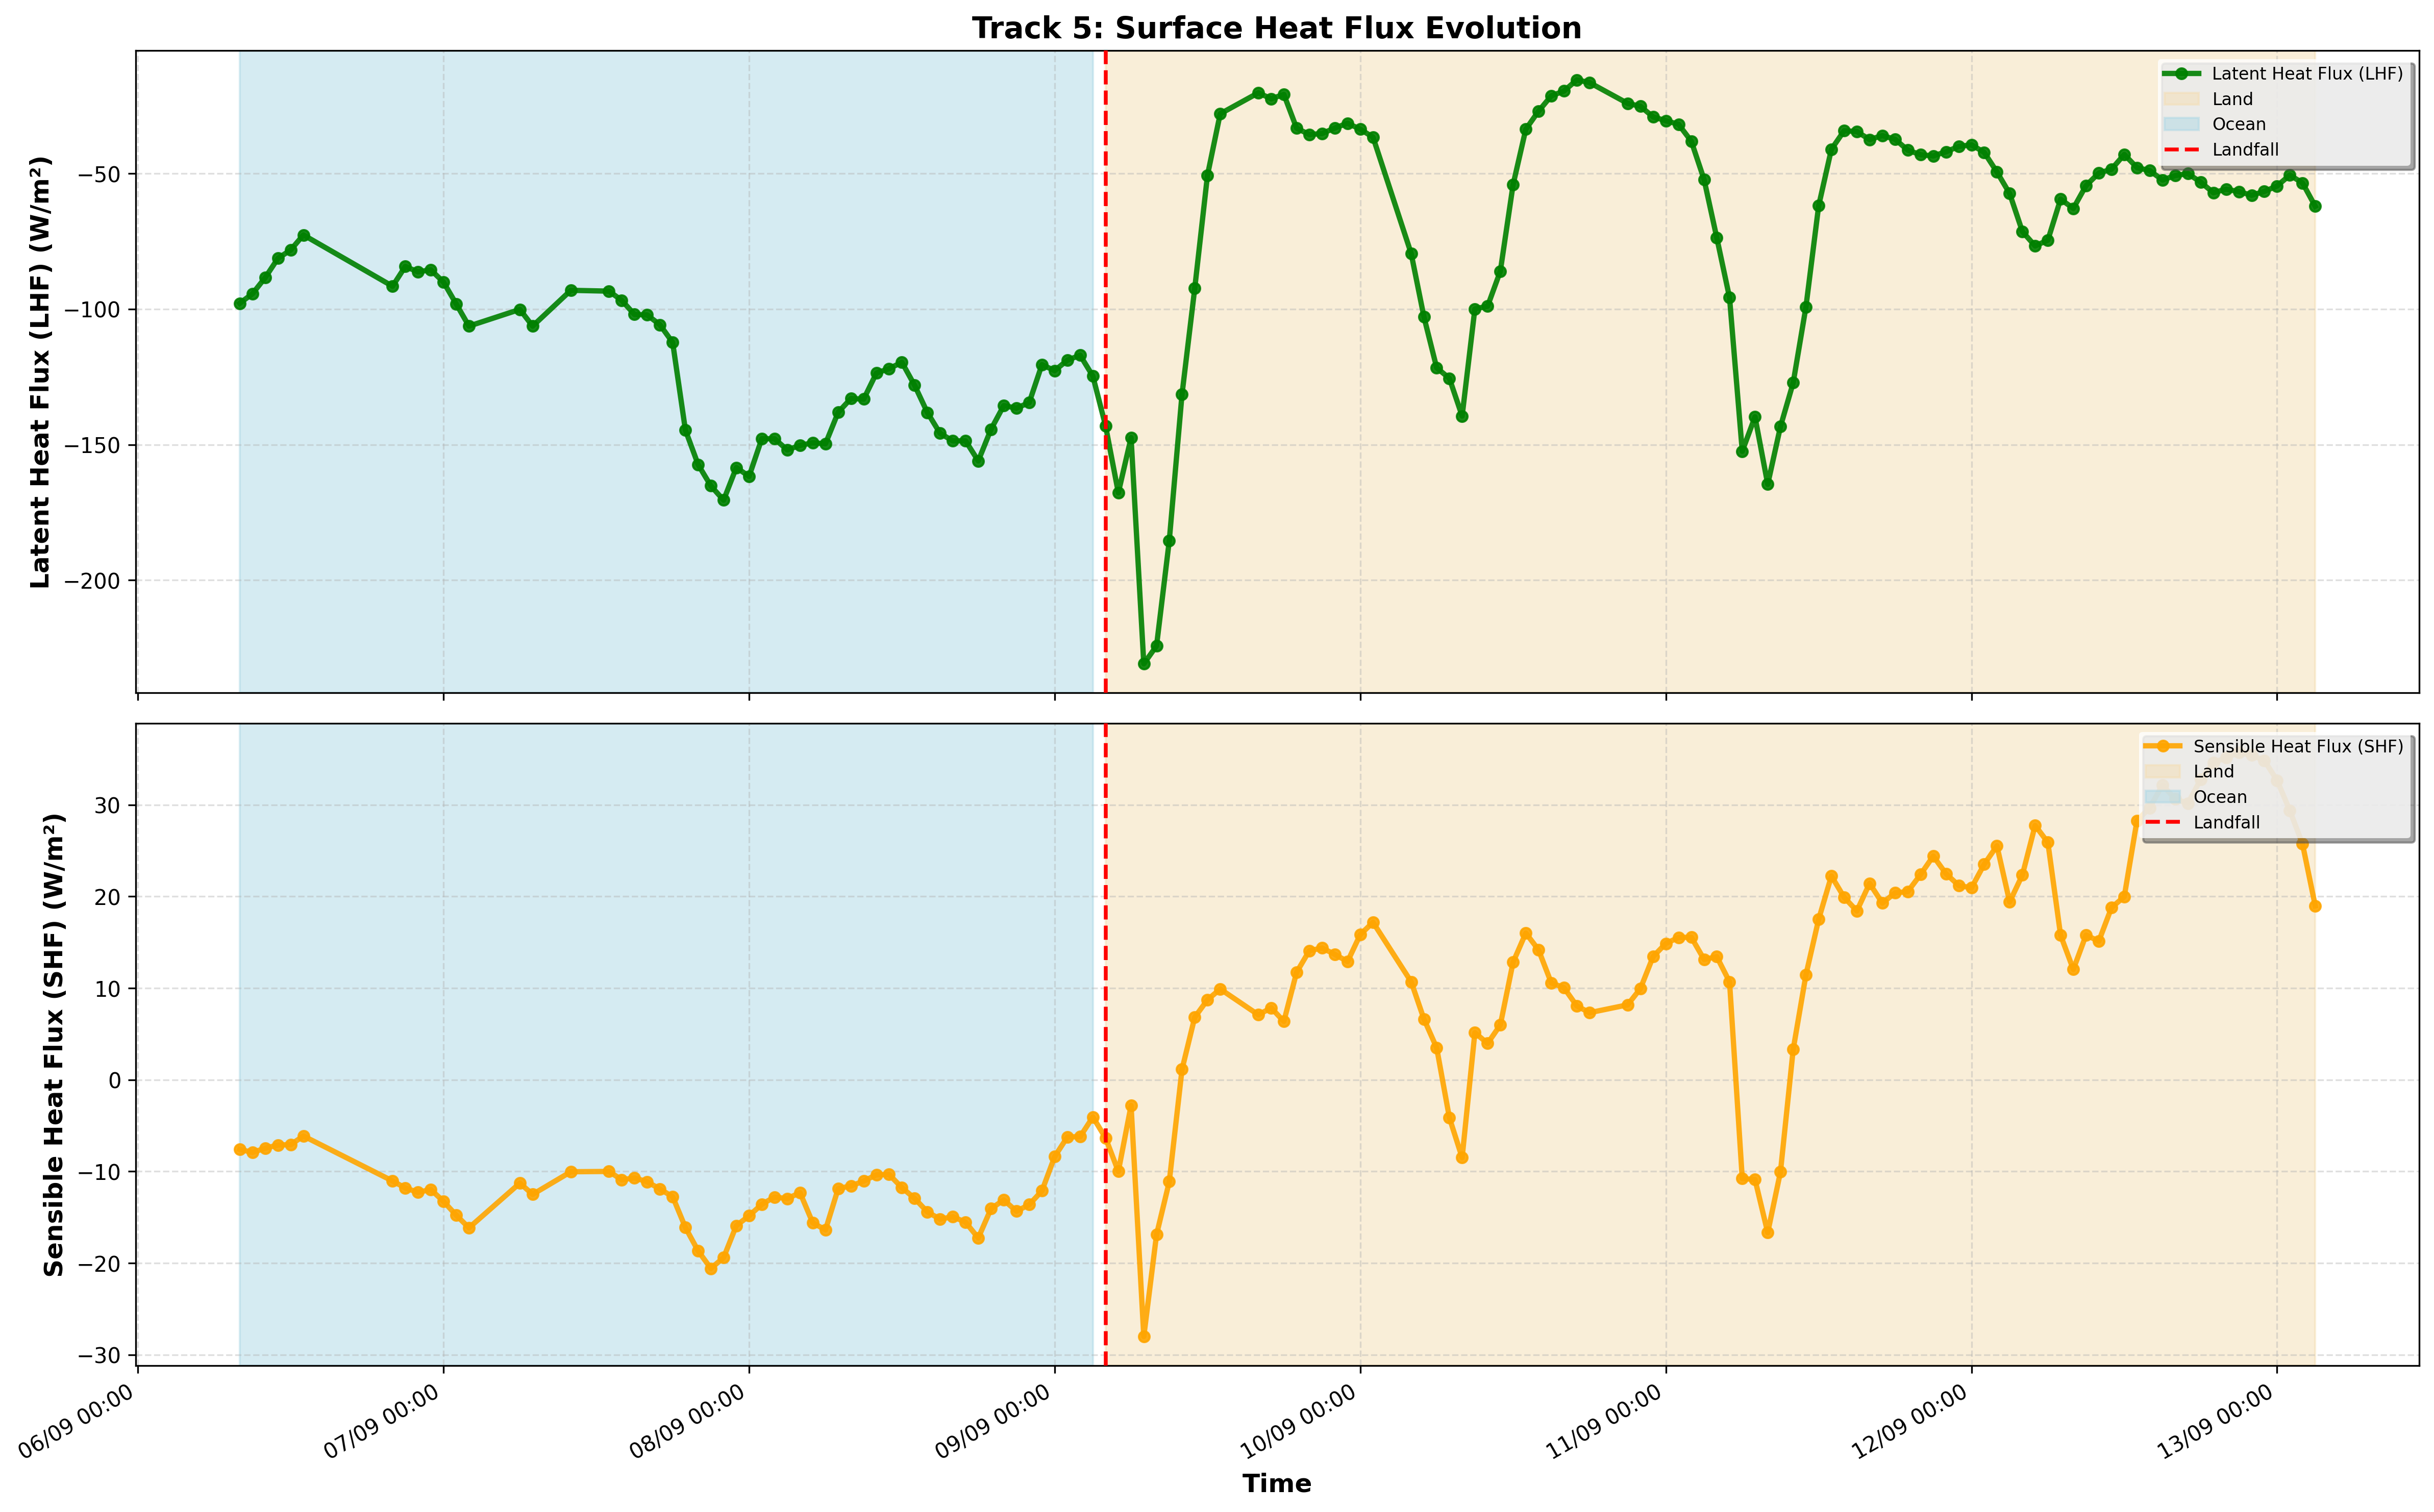
\includegraphics[width=\textwidth]{track_long_HF_time_series}
      \caption{\scriptsize \textbf{BOE-Active:} LHF exceeds
        150-200 W\,m$^{-2}$ pre-landfall; remains $\geq 70$ W\,m$^{-2}$ for
      $>72$ h inland. SHF fluctuates near zero, soil moisture prominent region}
    \end{figure}

    \column{0.50\textwidth}
    \vspace{-1.1cm}
    \begin{figure}
      \centering
      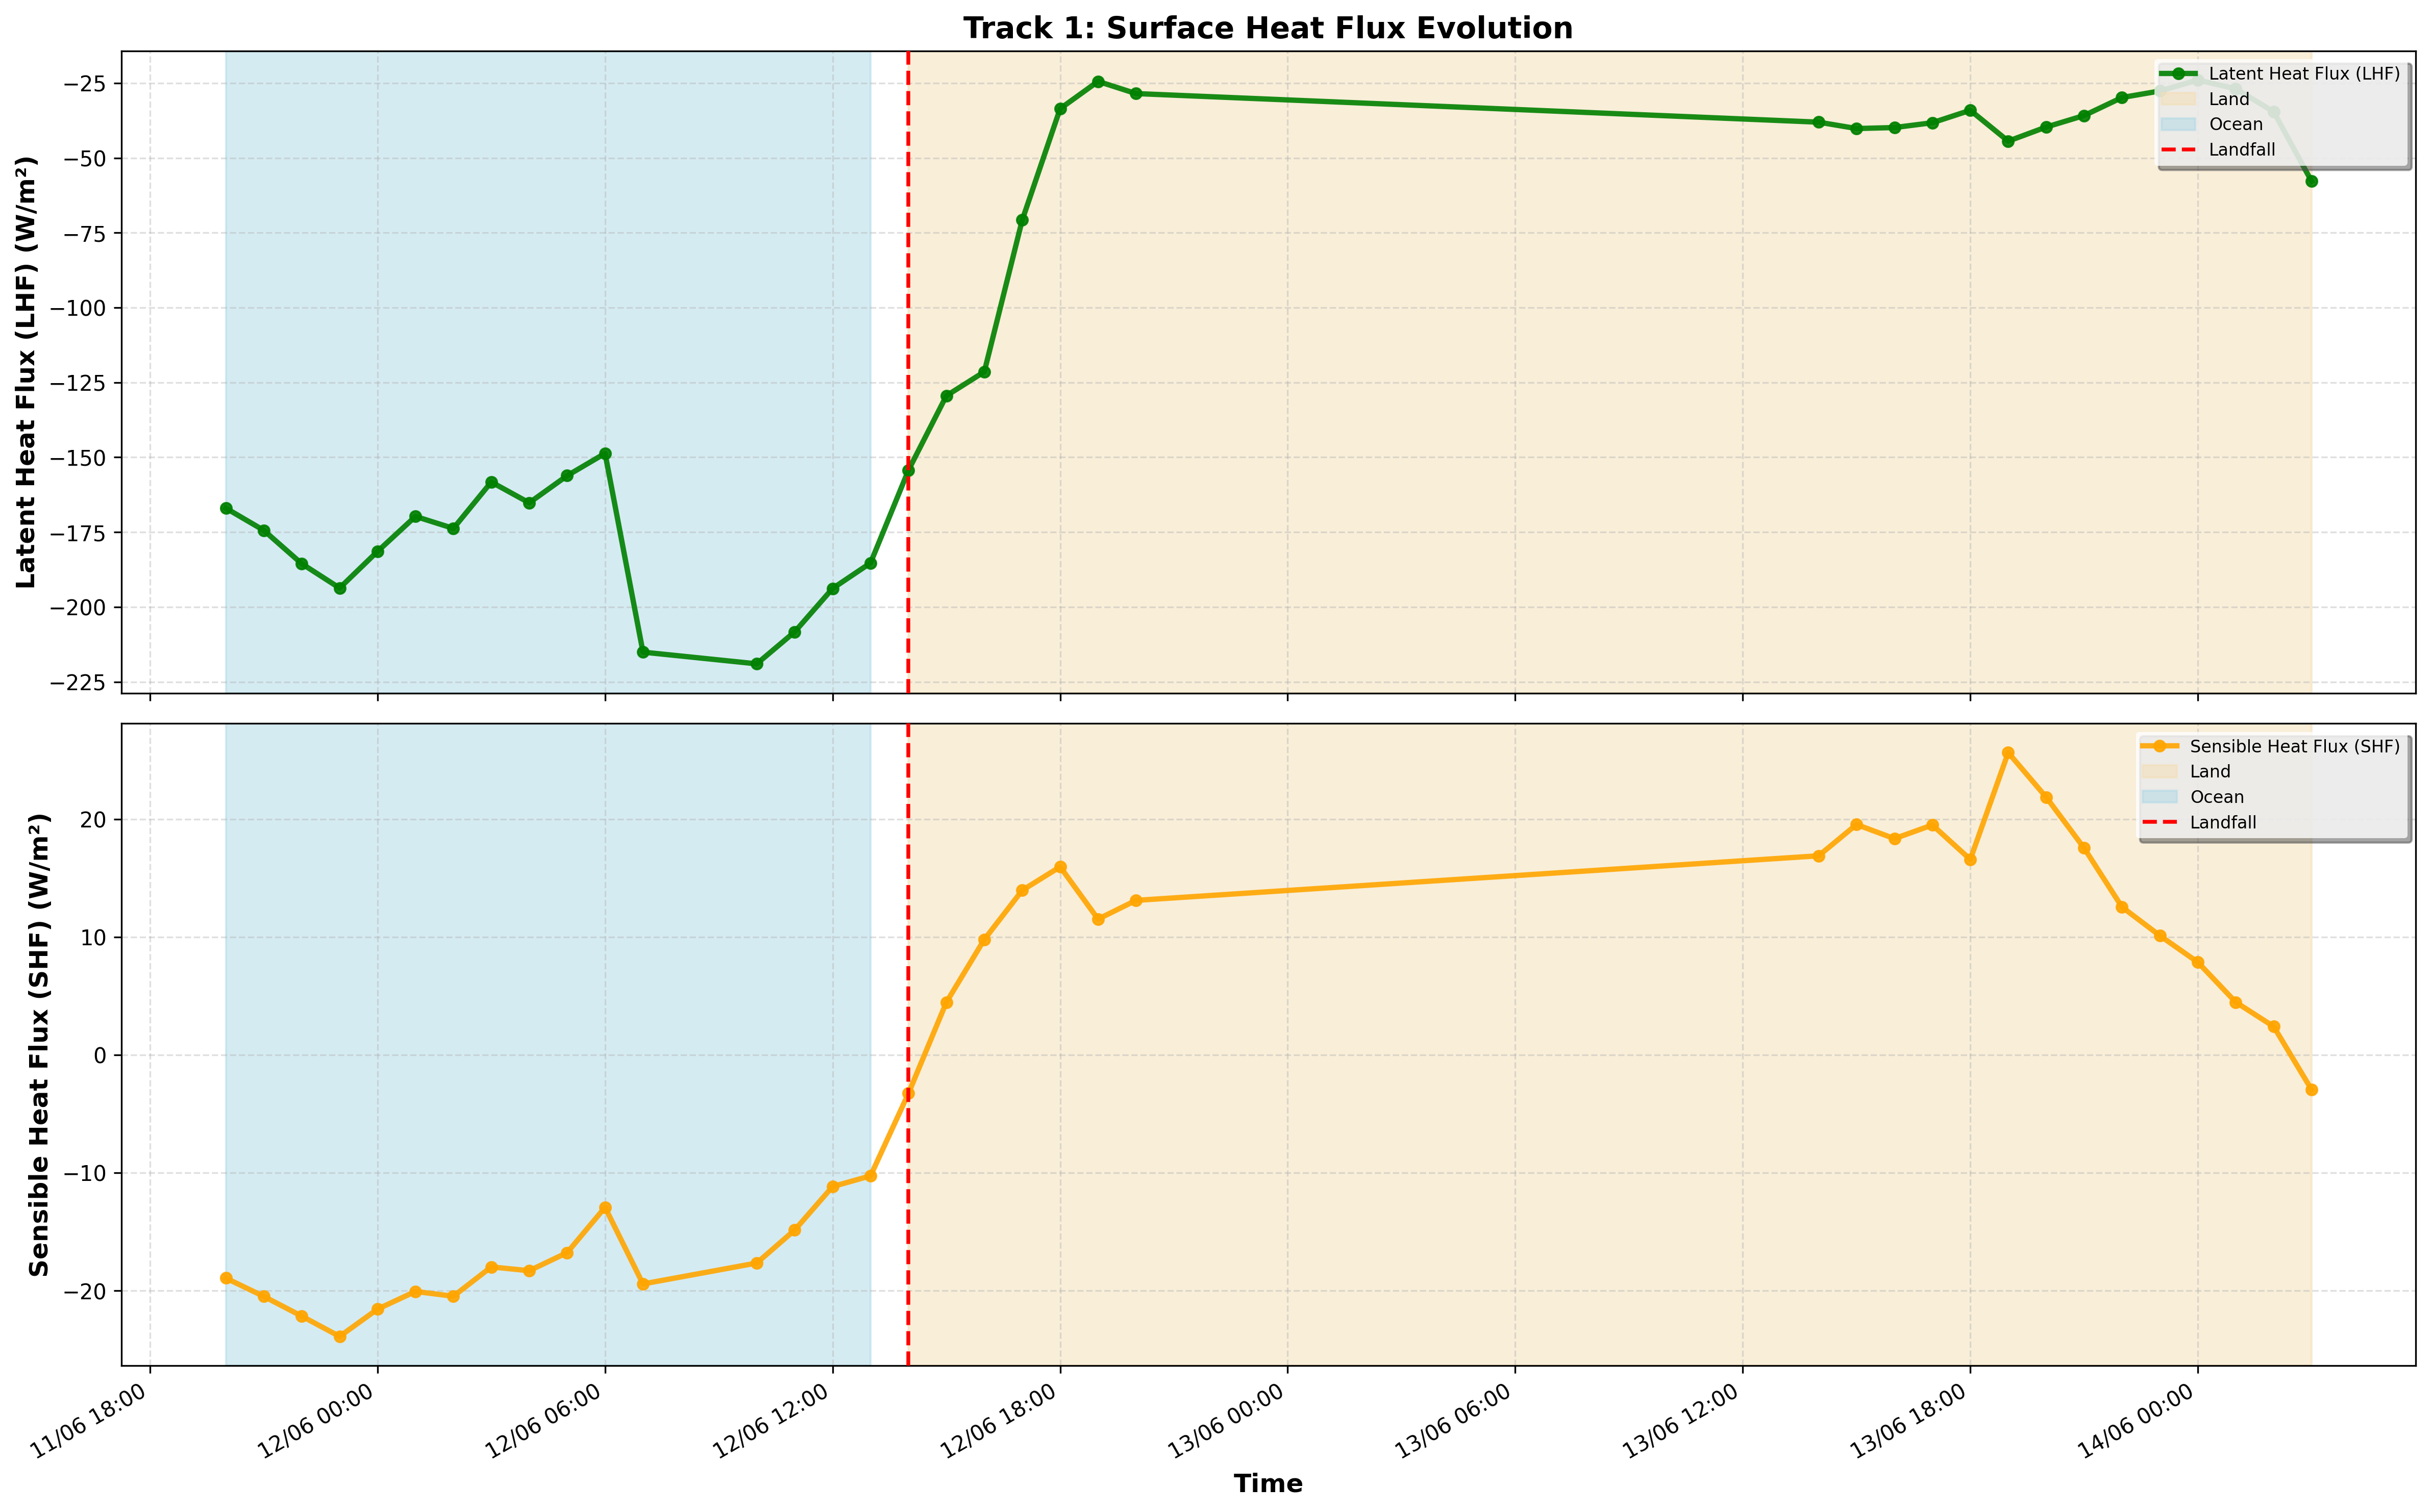
\includegraphics[width=\textwidth]{track_short_HF_time_series}
      \caption{\scriptsize \textbf{Non-BOE:} LHF stayed below 70
        W\,m$^{-2}$ within \textbf{12-18 h} of landfall. SHF $\gg$ 0,
      moisture-limited regime.}
    \end{figure}
  \end{columns}

  \vspace{-0.1cm}
  \footnotesize
  The Landfall Crossover : The sign and magnitude of SHF is the
  clearest single-variable indicator of regime: BOE $\Rightarrow$ SHF
  $\approx 0$; non-BOE $\Rightarrow$ SHF $\gg 0$. The surface energy
  budget determines whether the vortex maintains coupling between the
  low-level center and upper warm core.
\end{frame}

%---------------------------------------------------------Slide:
% Precipitation-Soil Moisture Feedback Loop
\setLayout{plain}
\begin{frame}{Precipitation-Soil Moisture Feedback: A Closed-Loop Diagnostic}
  \begin{columns}
    \column{0.50\textwidth}
    \vspace{-0.8cm}
    \begin{figure}
      \centering
      \includegraphics[width=\textwidth]{track_long_tp-swvl1_time_series}
      \caption{\footnotesize \textbf{BOE-Active:} Three-phase
        signature: (1) pre-conditioned landfall ($\geq 0.35$
        m$^3$\,m$^{-3}$), (2) intensive wetting phase (0-36 h), (3) phase
        synchronization - sustained 4 mm\,h$^{-1}$ drives SWVL1
        toward soil mositure holding
      capacity.}
    \end{figure}

    \column{0.50\textwidth}
    \vspace{-0.8cm}
    \begin{figure}
      \centering
      \includegraphics[width=\textwidth]{track_short_tp-swvl1_time_series}
      \caption{\footnotesize \textbf{Non-BOE:} Initial
        precipitation burst fails to establish feedback. Rapid surface
        desiccation ($t \approx 18$ h) prevents soil from reaching
      saturation - loop never activated.}
    \end{figure}
  \end{columns}

  \vspace{-0.1cm}
  \footnotesize
  The BOE is a threshold feedback. If the self-wetting loop
  is not activated within the \textbf{first 24 hours of landfall},
  the system inevitably undergoes structural decay - regardless of
  initial intensity.
\end{frame}

%---------------------------------------------------------Slide:
% Translational Speed
\setLayout{plain}
\begin{frame}{Translational Speed: Terrain Deceleration \& BOE Recovery}
  \begin{columns}
    \column{0.50\textwidth}
    \vspace{-1.0cm}
    \begin{figure}
      \centering
      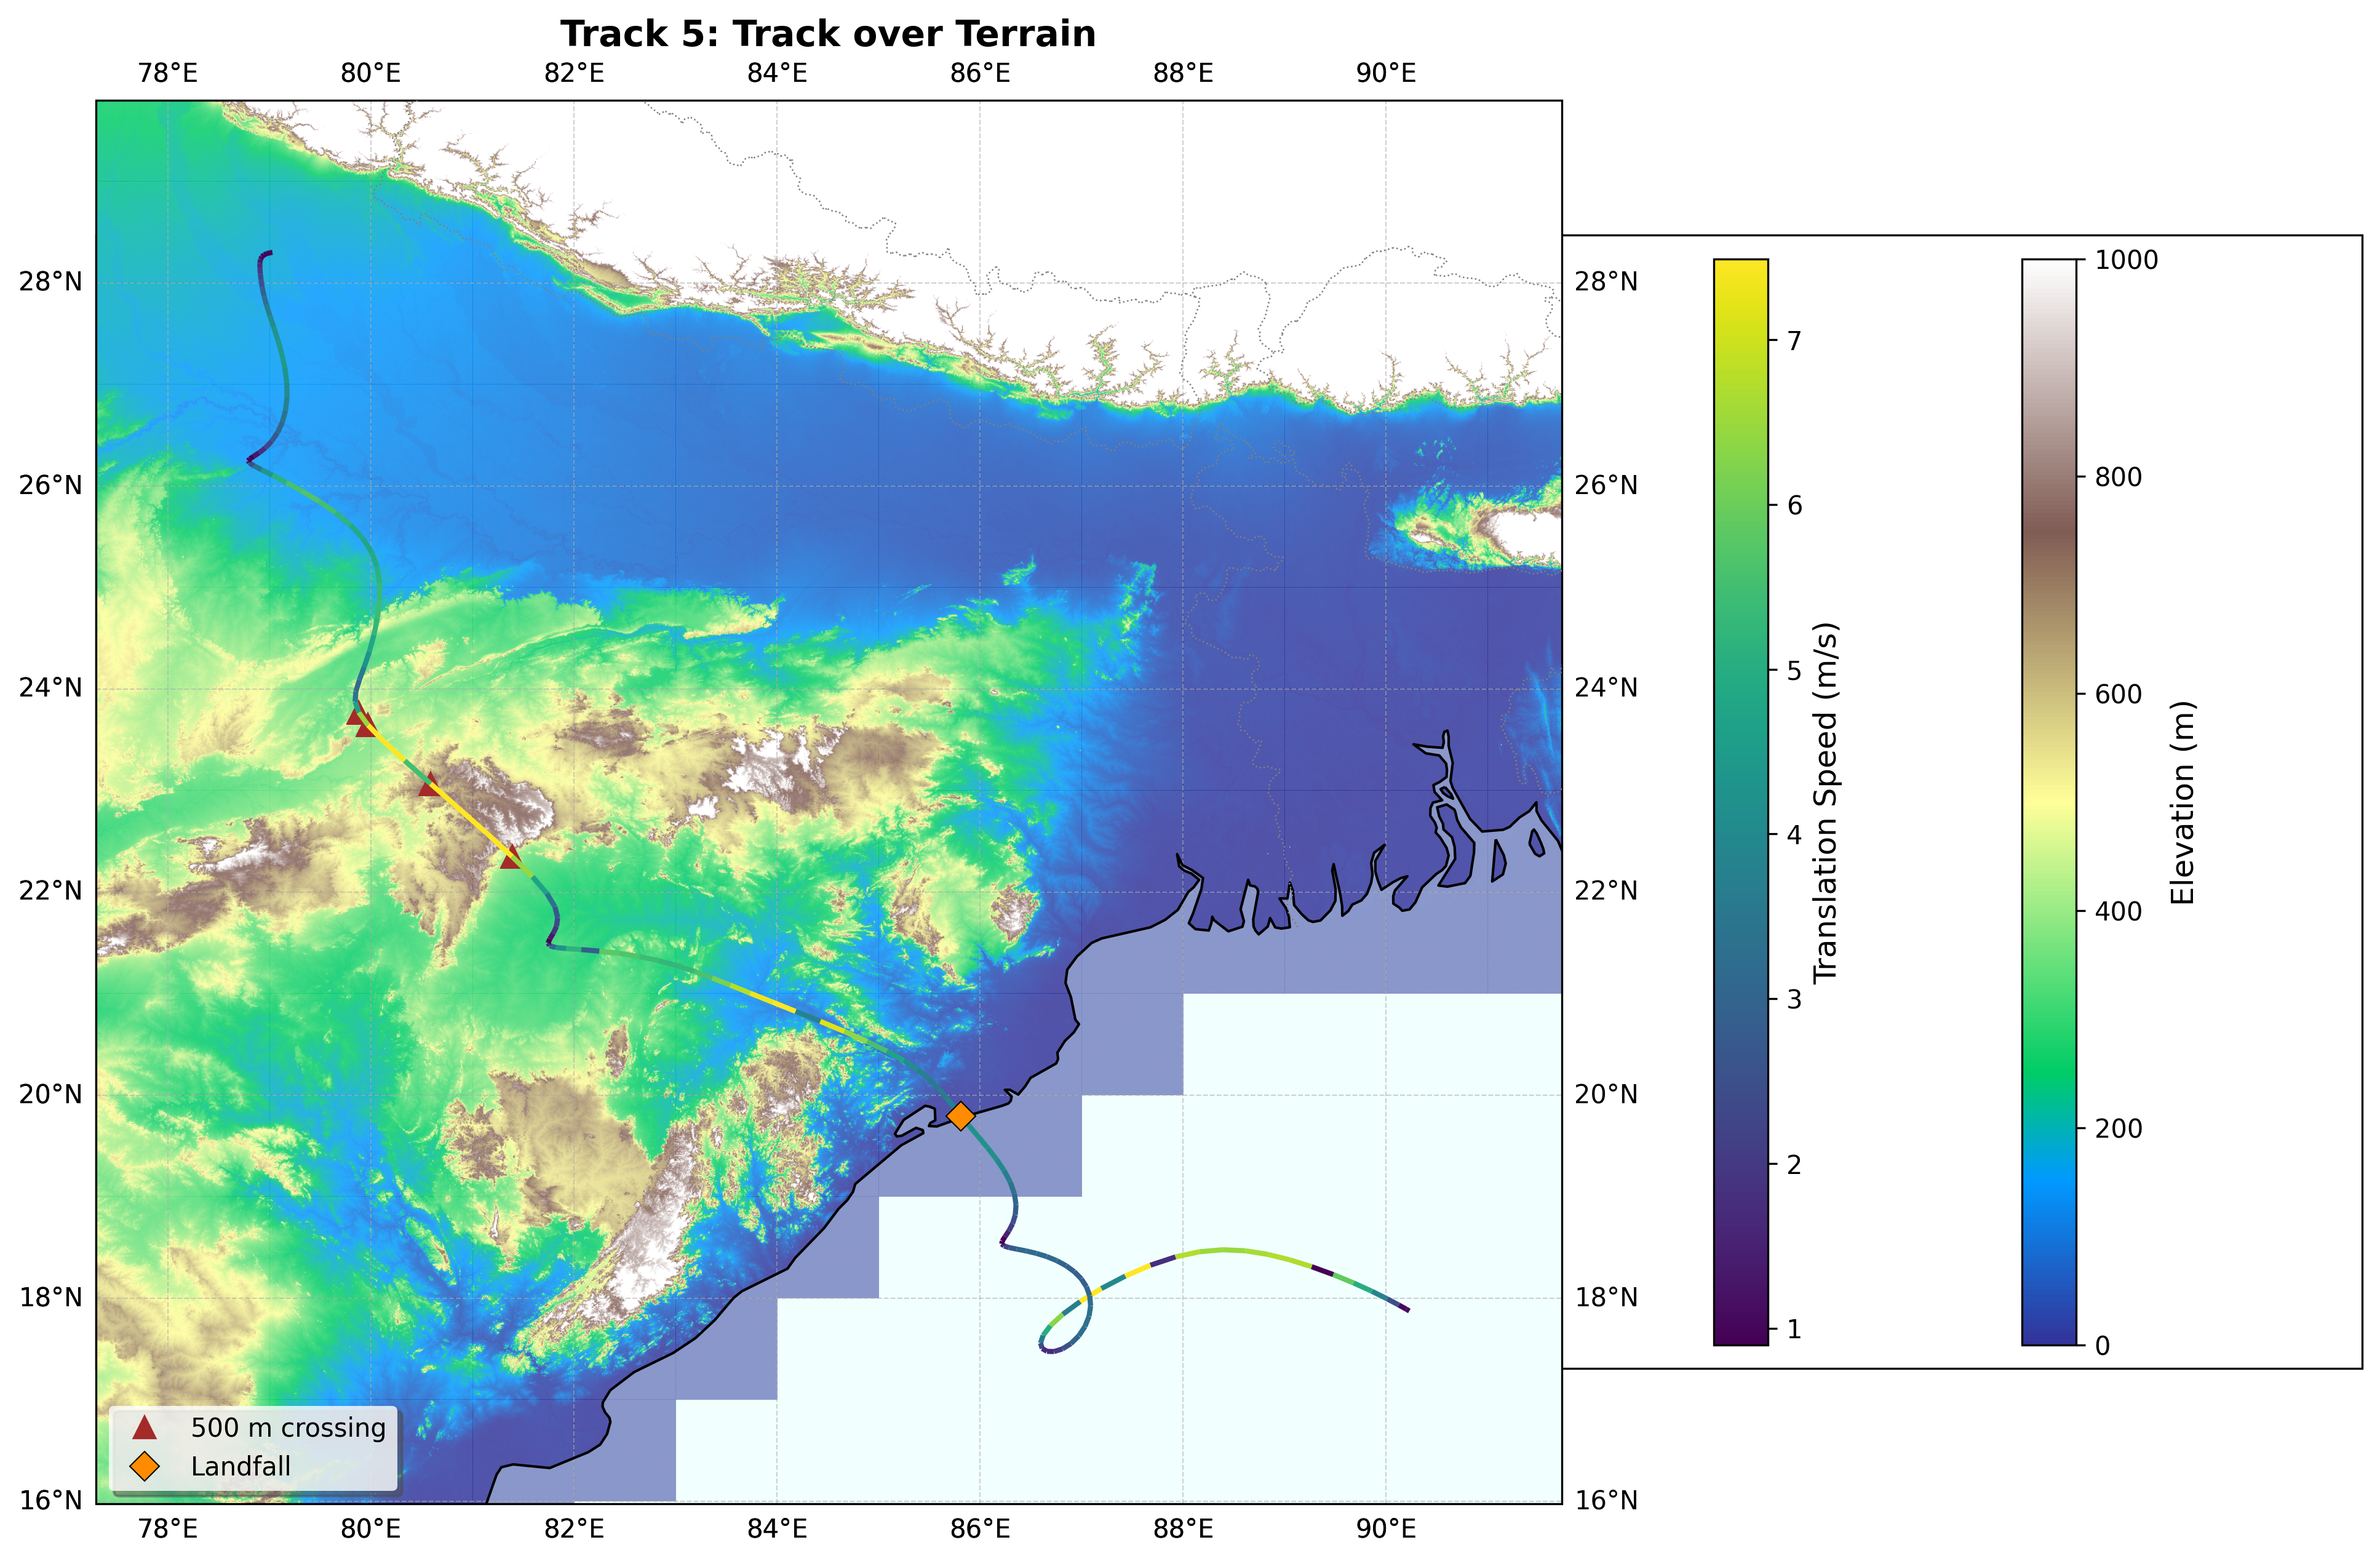
\includegraphics[width=0.95\textwidth]{track_long_elevation_speed_map}
      \caption{\footnotesize \textbf{BOE-Active:} Both systems
        decelerate at the terrain. Long-lived system exhibits clear
        \textbf{leeward speed recovery} - returns to $\sim$5 m\,s$^{-1}$
      west of the 500 m contour.}
    \end{figure}

    \column{0.50\textwidth}
    \vspace{-1.0cm}
    \begin{figure}
      \centering
      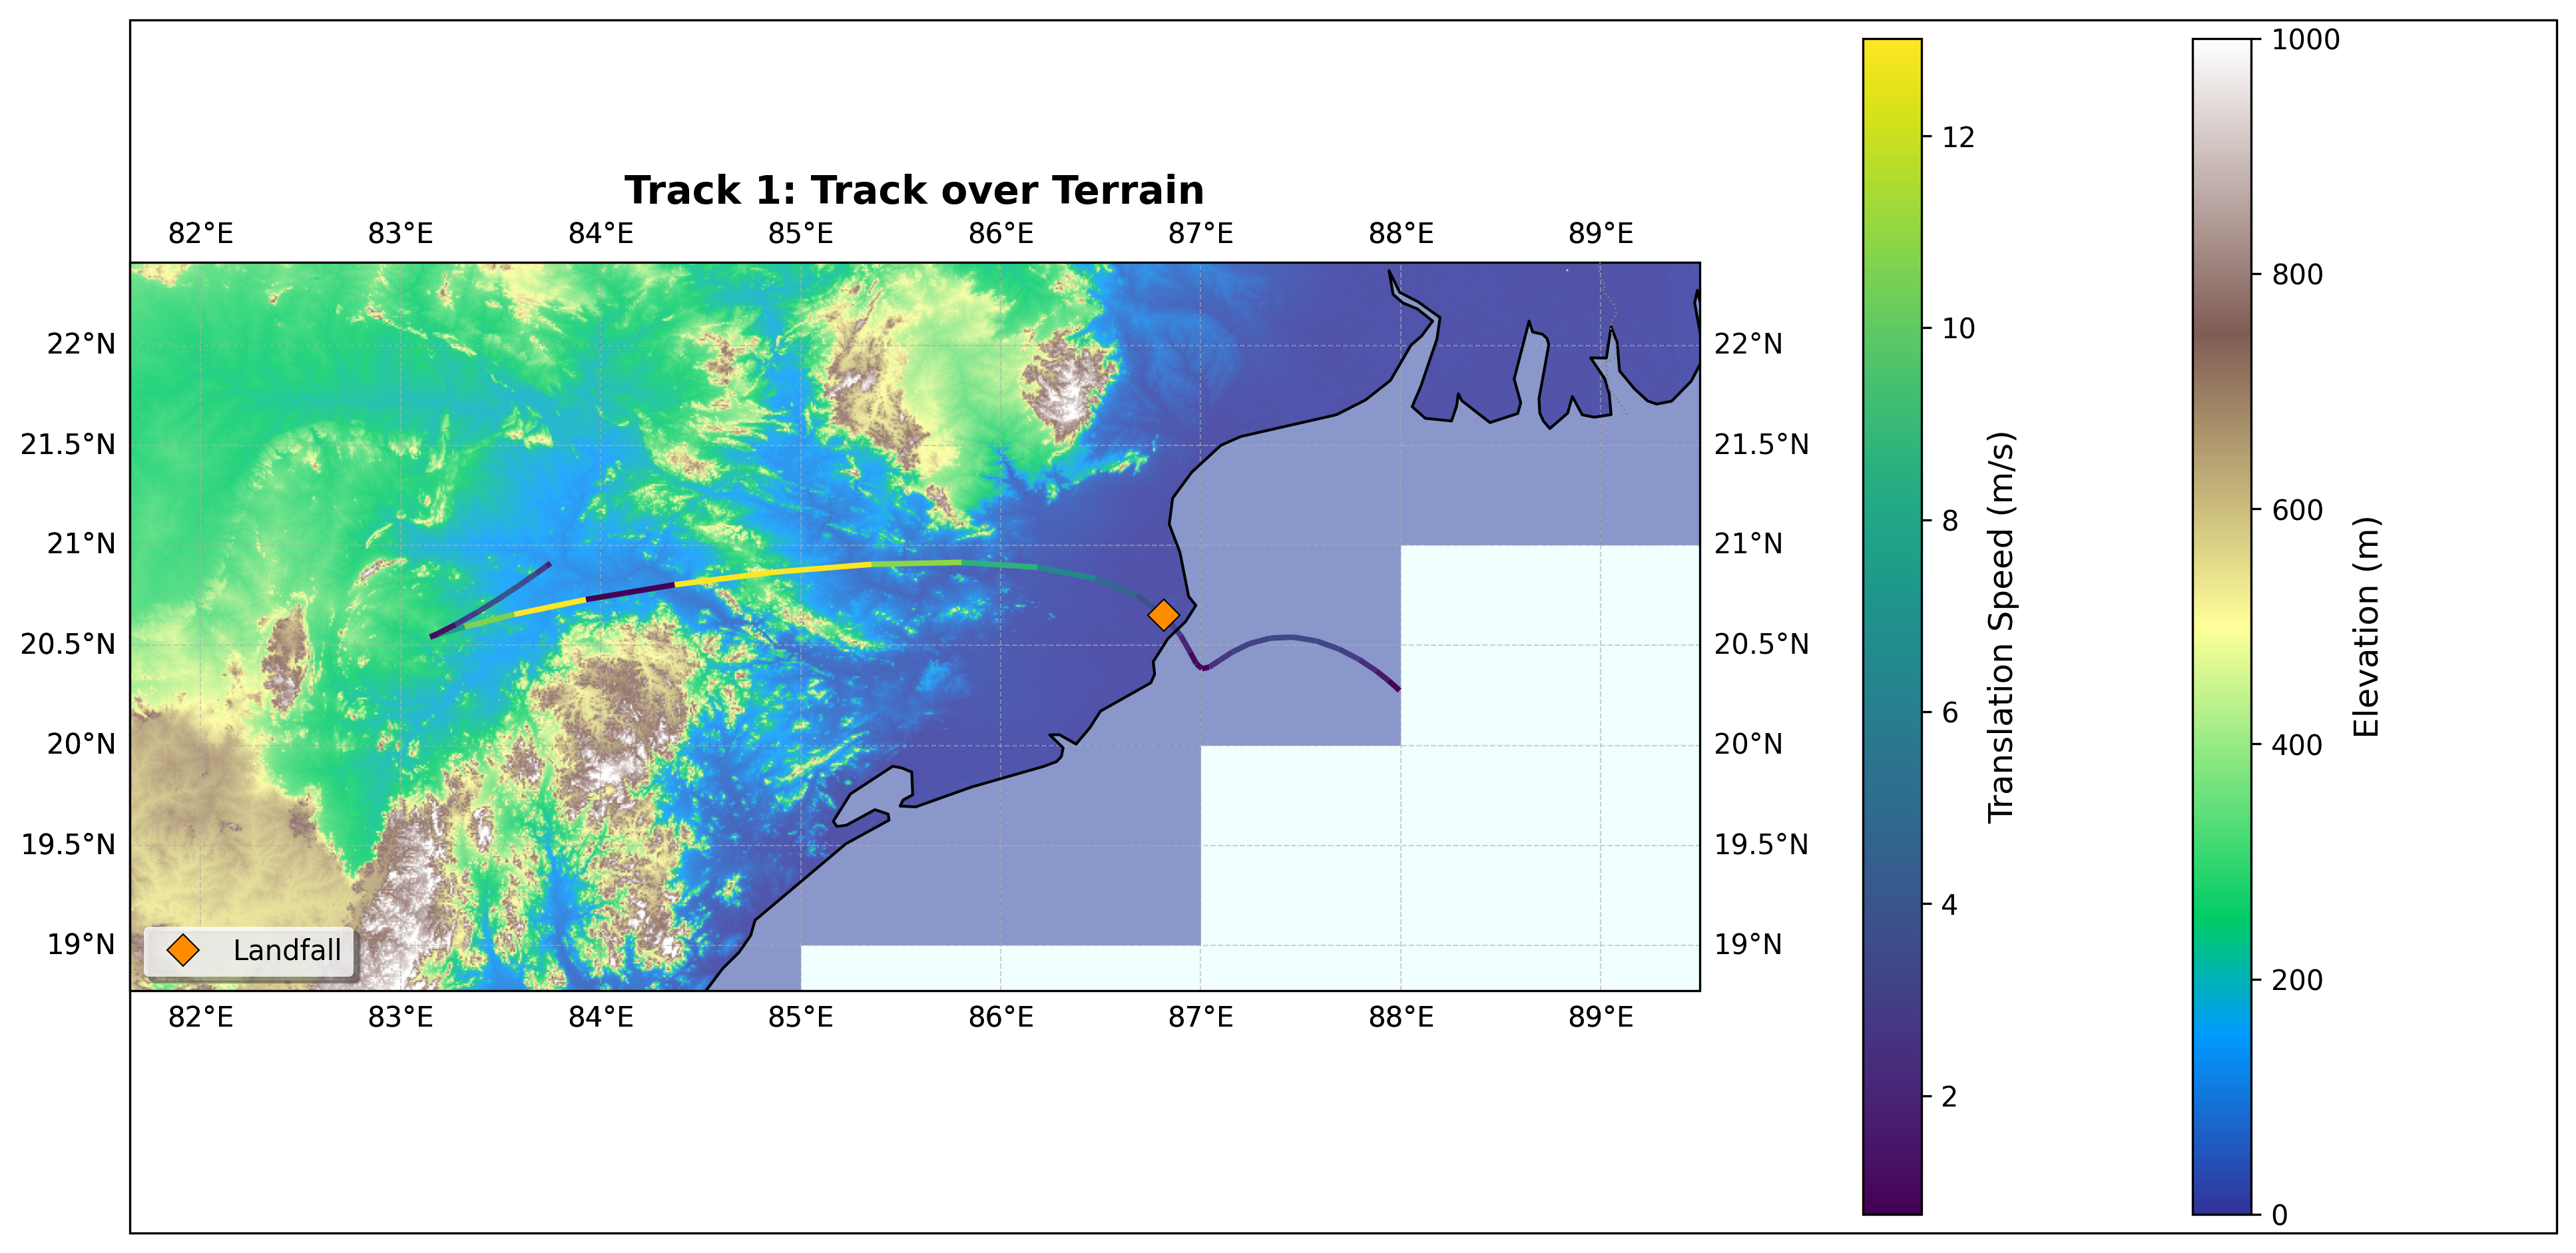
\includegraphics[width=1.1\textwidth]{track_short_elevation_speed_map}
      \caption{\footnotesize \textbf{Non-BOE:} Sustained
        deceleration without recovery - stalling behaviour and track
        termination on the windward or leeward slope. Convective vortex
      collapses during terrain-crossing.}
    \end{figure}
  \end{columns}

  \vspace{-0.1cm}
  \scriptsize
  Over the ocean, MDs translate at 6 m\,s$^{-1}$. Both systems
  decelerate at the Ghats from increased surface roughness and
  mechanical flow blocking. Only BOE-active systems re-accelerate:
  the sustained surface LHF (BOE engine) maintains the pressure
  gradient force required to drive the system forward on the leeward side.
\end{frame}

%---------------------------------------------------------Slide: Eastern Ghats Survivors
\setLayout{vertical}
\begin{frame}{Eastern Ghats Survivors: The BOE-Selective Filter}
  \begin{columns}
    \column{0.52\textwidth}
    \vspace{-0.8cm}
    \begin{figure}
      \centering
      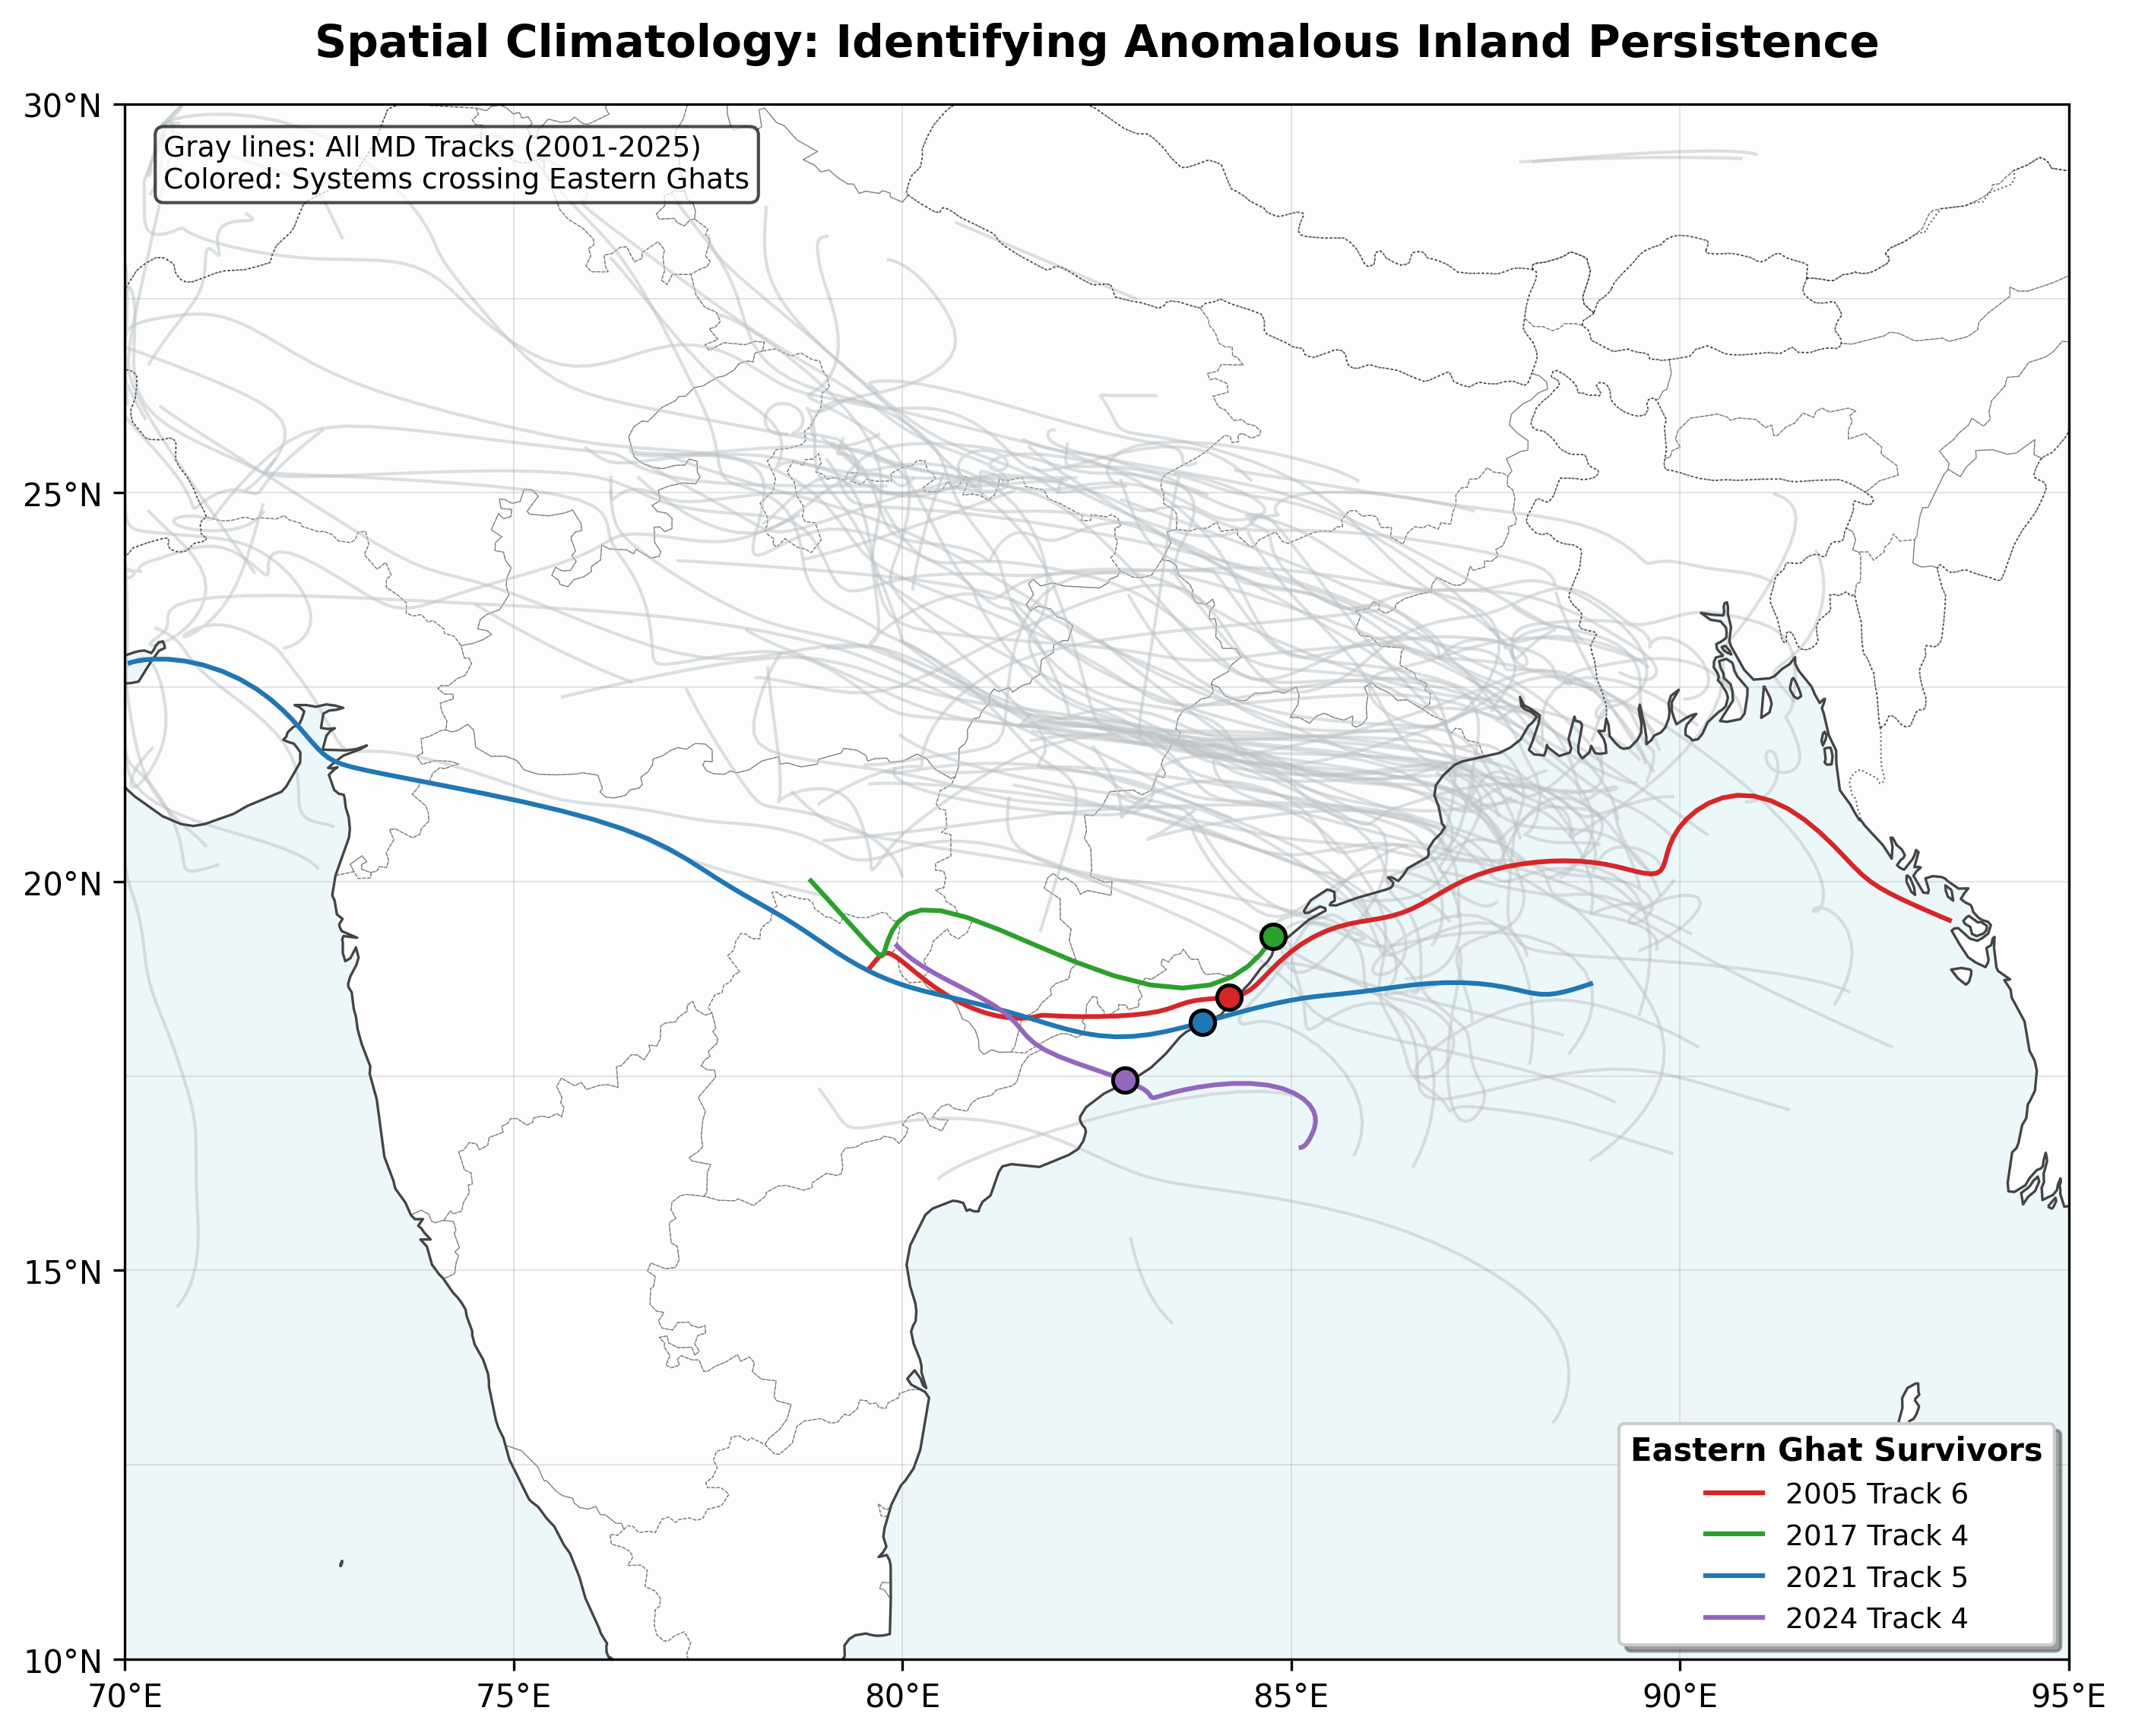
\includegraphics[width=0.95\textwidth]{ghats_survivors_map}
      \caption{\scriptsize Climatological MD termination points
        (grey) vs. the four anomalous survivor systems - \textbf{2005 (T6), 2017
        (T4), 2021 (T5), and 2024 (T4)} - that maintained MD-level intensity
      across the high-relief Eastern Ghats.}
    \end{figure}

    \column{0.47\textwidth}
    \vspace{0.6cm}

    \textbf{\small Observations:}
    \footnotesize
    \begin{itemize}
      \item The vast majority of MDs treat the Ghats as a
        \textbf{topographic wall} - terminating at or before the 500 m contour
      \item Four systems in the 2001-2025 dataset exhibit anomalous
        survival, all confirmed BOE-active
        %       \item Survivor landfall longitudes align with major
        % \textbf{river-valley gaps} (Mahanadi, Godavari corridors) -
        % low-level moisture inflow preserved
    \end{itemize}

    \vspace{0.2cm}
    \footnotesize
    The Eastern Ghats do not uniformly block MDs. They
    selectively eliminate non-BOE systems and act only as a
    \textbf{moderate obstacle} when BOE is active. Land-atmosphere
    coupling is the primary determinant of inland penetration.
  \end{columns}
\end{frame}

% SECTION IV - Conclusions
\section{Conclusions}
\setLayout{mainpoint}
\begin{frame}{}
  \frametitle{Conclusions}
\end{frame}

%---------------------------------------------------------Slide: Conclusions 1
% BOE Synthesis
\setLayout{vertical}
\begin{frame}{BOE as a Diagnostic Mechanism: Four Synchronized Signatures}
  \footnotesize
  In every confirmed long-lived event, four independent
  observational signals converge at landfall:

  \begin{columns}
    \column{0.46\textwidth}
    \begin{block}{\small Signal 1: Inward Contraction}
      \footnotesize
      Precipitation maximum shifts from a broad maritime footprint
      to a \textbf{concentrated inner core ($<100$ km)} - the storm feeds
      itself rather than relying on large-scale moisture advection.
    \end{block}

    \vspace{0.2cm}

    \begin{block}{\small Signal 2: Self-Wetting Persistence}
      \footnotesize
      Core rainfall maintains a \textbf{saturated soil reservoir
      ($>0.40$ m$^3$\,m$^{-3}$)}, preventing the surface desiccation that
      normally follows landfall. The storm conditions its own energy source.
    \end{block}

    \column{0.50\textwidth}
    \begin{block}{\small Signal 3: Oceanic-Scale Fluxes}
      \footnotesize
      Land-phase LHF remains above the sustaining threshold
      (\textbf{$>70$ W\,m$^{-2}$}), effectively mimicking the energy
      environment of the Bay of Bengal it just left.
    \end{block}

    \vspace{0.2cm}

    \begin{block}{\small Signal 4: Thermodynamic Stability}
      \footnotesize
      Energy partitioned into evaporation rather than sensible
      heating (\textbf{low Bowen ratio}). Cool, moist boundary layer and
      low LCL preserve the vortex column coupling - the storm's warm core
      stays anchored.
    \end{block}
  \end{columns}

  \vspace{0.2cm}
  \begin{alertblock}{\small The Predictive Paradox}
    \footnotesize
    Mechanical factors (Eastern Ghats) modulate the translational
    speed of \textbf{all} systems. Only BOE-active systems exhibit
    leeward speed recovery. \textbf{Thermodynamic energy supply from
    land-atmosphere coupling is the primary determinant of inland penetration.}
  \end{alertblock}
\end{frame}

% CONCLUSIONS
\section{Conclusions}

%---------------------------------------------------------Slide: Conclusions 2
\setLayout{vertical}
\begin{frame}{Principal Conclusions}
  \footnotesize
  \begin{enumerate}
    \item \textbf{The BOE discriminates long-lived from short-lived systems.}
      Of 128 confirmed land-falling MDs (2001-2025), \textbf{38
      systems (29.7\%)} meet the BOE criterion. Importantly \textbf{all
        38 BOE-candidate systems are long-lived ($\geq 96$ h, mean 138.3
      h); no short-lived system qualifies}. This demonstrates the BOE
      is a \textit{necessary condition} for anomalous inland persistence.

      \vspace{0.2cm}

    \item \textbf{The Azimuthal Hovmöller captures the transition
      to land-based energy.}
      Long-lived MDs exhibit a distinct Hovmöller signature:
      \textit{inward contraction} of precipitation to the inner core
      ($<100$ km), sustained inner-core LHF, and near-saturated BL (Dew
      Point Depression $<3$ K). This confirms the system has switched
      from oceanic moisture to local surface evapotranspiration.

      \vspace{0.2cm}

    \item \textbf{The Eastern Ghats act as a thermodynamic filter,
      not an absolute barrier.}
      Both long-lived and short-lived systems decelerate at the
      terrain, but display different leeward behaviour: BOE-active
      systems recover translational speed on the leeward side, while
      non-BOE systems continue to decelerate and decay. River-valley
      gap alignment (Mahanadi, Godavari corridors) further
      enhances penetration.
  \end{enumerate}
\end{frame}

%---------------------------------------------------------Slide: Conclusions 3
\setLayout{vertical}
\begin{frame}{Principal Conclusions (cont.)}
  \footnotesize
  \begin{enumerate}
      \setcounter{enumi}{3}
    \item \textbf{A self-wetting feedback loop maintains the inland
      depression core.}
      Time evolution of SWVL1 and precipitation in track-following diagnostics confirms an active positive feedback:
      MD rainfall increases soil moisture, which sustains LHF above $70$
      W\,m$^{-2}$, which drives subsequent deep convection. This
      mechanism allows the atmosphere to maintain oceanic-like convective
      organisation over land. If this loop is not activated within the
      \textbf{first 24 hours of landfall}, the system eventually decays.
  \end{enumerate}

  \vfill
  % \vspace{0.3cm}

  \begin{block}{\small Significance}
    \footnotesize
    This research provides the systematic \textbf{storm-centred} observational evidence for the BOE in Indian Monsoon Depressions. Prior work relied on NWP experiments or fixed-grid correlations. The Azimuthal Hovmöller framework offers a
    MD-centred diagnostic capable of distinguishing BOE-active from BOE-inactive systems - applicable in real time to ERA5T or regional NWP output.
  \end{block}
\end{frame}

% %---------------------------------------------------------Slide: Future Work
% \setLayout{vertical}
% \begin{frame}{Future Work \& Operational Applications}
%   \begin{columns}
%     \column{0.50\textwidth}
%     \textbf{\small Directions for Future Research:}
%     \footnotesize
%     \begin{enumerate}
%       \item \textbf{3D vortex diagnostics} - pressure-level
% analyses of warm/cold-core evolution, vorticity column coherence,
% IVT, and vortex tilt to provide a dynamical counterpart to the
% surface thermodynamic evidence
%
%       \item \textbf{Multi-reanalysis cross-validation} - repeat
% Hovmöller analysis with MERRA-2 and JRA-55; assess sensitivity to
% differing land-surface parameterisations (HTESSEL vs. CLSM vs. JMA scheme)
%
%       \item \textbf{Eastern Ghats gap-passage analysis} -
% systematic test of landfall longitude relative to Godavari,
% Mahanadi, and Brahmani river-valley gaps
%
%       \item \textbf{NWP sensitivity experiments} - targeted
% WRF/Unified Model runs with perturbed soil moisture initialisation
% for identified BOE-candidate events
%     \end{enumerate}
%
%     \column{0.48\textwidth}
%     \textbf{\small Operational Applications:}
%     \footnotesize
%     \begin{itemize}
%       \item The Azimuthal Hovmöller framework can be applied in
% \textbf{near-real-time} using ERA5T data or regional NWP output to
% assess post-landfall evolution at landfall time
%       \item The multi-variable BOE signature (inner-core LHF, SWVL1
% progressive wetting, DPD near-saturation, precipitation
% contraction) provides an operationally accessible fingerprint
%       \item A simple \textbf{soil moisture index at landfall} could
% give district-level flood forecast agencies an additional
% \textbf{48-72 h of warning} for evacuation and pre-positioning of
% relief supplies
%     \end{itemize}
%
%     \vspace{0.2cm}
%     \begin{alertblock}{\small Climate Outlook}
%       \scriptsize
%       As monsoon patterns shift under climate change and irrigation
% intensifies, favourable BOE conditions may intensify or diminish -
% determining whether India's most significant inland weather systems
% become more or less dangerous in the decades ahead.
%     \end{alertblock}
%   \end{columns}
% \end{frame}

% REFERENCES
\section{References}
\setLayout{horizontal}
\begin{frame}[allowframebreaks]
    \frametitle{References}
    \nocite{*}
    \bibliographystyle{IEEEtran}
    \tiny
    \bibliography{references}
\end{frame}

% THANK YOU
\section{End}
\setLayout{blank}
\begin{frame}
  \centering
  \vspace{3.0cm}
  \textbf{\Huge Thank You} \\
  \vspace{0.8cm}
  \textbf{\large Questions \& Suggestions}
  \vspace{1.5cm}

  \footnotesize
  \begin{columns}
    \column{0.4\textwidth}
    \centering
    \textbf{Harshit Prashant Dhanwalkar} \\
    SC21B164
    \column{0.4\textwidth}
    \centering
    \textbf{Supervisor:} Dr. A. Chandrasekar \\
    Dept. of Earth \& Space Sciences, IIST
  \end{columns}
\end{frame}

\end{document}
